%===============================================================
% BioAlerta: Informe de Proyecto — Borrador
% Compilar con: pdflatex informe_bioalerta.tex (dos veces)
% Requiere: MiKTeX con paquetes listings, booktabs, longtable,
%           tikz, pgfplots, hyperref, babel-spanish, geometry
%===============================================================
\documentclass[12pt,a4paper]{article}

% ---- Codificación y lengua ----
\usepackage[utf8]{inputenc}
\usepackage[T1]{fontenc}
% Para hifenación correcta en español: sudo dnf install texlive-babel-spanish
% y cambiar la siguiente línea a: \usepackage[spanish,es-tabla]{babel}
\usepackage[english]{babel}
\addto\captionsenglish{%
  \renewcommand{\contentsname}{Índice}%
  \renewcommand{\figurename}{Figura}%
  \renewcommand{\tablename}{Tabla}%
  \renewcommand{\appendixname}{Anexo}%
  \renewcommand{\refname}{Referencias}%
}

% ---- Márgenes ----
\usepackage[top=2.5cm, bottom=2.5cm, left=3cm, right=2.5cm]{geometry}

% ---- Tipografía ----
\usepackage{lmodern}
\usepackage{microtype}

% ---- Matemáticas ----
\usepackage{amsmath,amssymb}

% ---- Colores ----
\usepackage[dvipsnames,svgnames,table]{xcolor}
\definecolor{azulBio}{RGB}{30,90,160}
\definecolor{verdeBio}{RGB}{46,125,50}
\definecolor{rojoBio}{RGB}{183,28,28}
\definecolor{grisCelda}{RGB}{240,245,250}

% ---- Gráficos y figuras ----
\usepackage{graphicx}
\usepackage{float}
\usepackage{caption}
\captionsetup{font=small, labelfont=bf}

% ---- TikZ para diagramas ----
\usepackage{tikz}
\usetikzlibrary{shapes.geometric, arrows.meta, positioning, fit,
                decorations.pathreplacing, calc, backgrounds, shadows}

% ---- Tablas ----
\usepackage{booktabs}
\usepackage{longtable}
\usepackage{array}
\usepackage{tabularx}
\usepackage{colortbl}

% ---- Código fuente ----
\usepackage{listings}
\lstset{
  basicstyle=\ttfamily\footnotesize,
  backgroundcolor=\color{grisCelda},
  frame=single,
  breaklines=true,
  captionpos=b,
  keywordstyle=\color{azulBio}\bfseries,
  commentstyle=\color{verdeBio},
  stringstyle=\color{rojoBio},
  language=Python,
  numbers=left,
  numberstyle=\tiny\color{gray},
  numbersep=5pt
}

% ---- Hipervínculos ----
\usepackage[colorlinks=true, linkcolor=azulBio, citecolor=verdeBio,
            urlcolor=azulBio, bookmarks=true]{hyperref}

% ---- Encabezados ----
\usepackage{fancyhdr}
\setlength{\headheight}{14pt}
\pagestyle{fancy}
\fancyhf{}
\fancyhead[L]{\small BioAlerta --- Borrador}
\fancyhead[R]{\small \thepage}
\renewcommand{\headrulewidth}{0.4pt}

% Evitar overfull hbox en texto normal (sin babel-spanish no hay patrones de guionado)
\emergencystretch=3em

% ---- Espaciado ----
\usepackage{setspace}
\onehalfspacing

% ---- Secciones con color ----
\usepackage{titlesec}
\titleformat{\section}{\large\bfseries\color{azulBio}}{\thesection.}{0.5em}{}[\titlerule]
\titleformat{\subsection}{\normalsize\bfseries\color{azulBio}}{\thesubsection.}{0.5em}{}
\titleformat{\subsubsection}{\normalsize\itshape\color{azulBio}}{\thesubsubsection.}{0.5em}{}

% ---- Enumeraciones ----
\usepackage{enumitem}

%===============================================================
% INICIO DEL DOCUMENTO
%===============================================================
\begin{document}

%---------------------------------------------------------------
% CARÁTULA
%---------------------------------------------------------------
\begin{titlepage}
  \thispagestyle{empty}
  \singlespacing
  \centering

  \vspace*{0.5cm}

  {\Large\bfseries Universidad Mayor de San Andrés}\\[0.3em]
  {\normalsize Facultad de Ciencias Puras y Naturales}\\[0.15em]
  {\normalsize Carrera de Informática}

  \vspace{0.5cm}

  
\includegraphics[width=2.8cm]{img/Logo_Umsa.png}

  \vspace{0.6cm}

  {\color{azulBio}\rule{\linewidth}{1.5pt}}
  \vspace{0.35cm}

  {\LARGE\bfseries BioAlerta}\\[0.35em]
  {\large Predicción del Riesgo de Extinción\\[0.15em]
   de Especies Nativas de Bolivia\\[0.15em]
   mediante Aprendizaje Automático Supervisado}

  \vspace{0.35cm}
  {\color{azulBio}\rule{\linewidth}{1.5pt}}

  \vspace{0.7cm}

  {\large Maximiliano Gómez Mallo}\\[0.15em]
  {\normalsize 14480221}

  \vspace{0.7cm}

  \begin{tabular}{ll}
    \textbf{Materia:}  & Machine Learning              \\[0.25em]
    \textbf{Docente:}  & Menfy Morales Rios            \\[0.25em]
    \textbf{Fecha:}    & La Paz, Bolivia --- Marzo 2026 \\
  \end{tabular}

\end{titlepage}

%---------------------------------------------------------------
% TABLA DE CONTENIDOS
%---------------------------------------------------------------
\tableofcontents
\newpage

%===============================================================
\section{Introducción}
%===============================================================

Bolivia es uno de los países con mayor diversidad biológica del planeta, albergando más de
\textbf{1\,718 especies de aves y mamíferos} registradas en bases de datos públicas.
Sin embargo, una fracción significativa de esa riqueza carece de evaluación formal de riesgo de extinción:
la \textit{Lista Roja de la IUCN} (\textit{International Union for Conservation of Nature})
no incluye a \textbf{202 especies} que habitan territorio boliviano.
Esta brecha de información impide que organizaciones gubernamentales, ONGs y tomadores de decisiones
prioricen acciones de conservación con criterios cuantitativos.

El presente proyecto, denominado \textbf{BioAlerta}, construye un \textit{pipeline} completo de
aprendizaje automático supervisado para: (1) identificar qué factores ambientales, geoespaciales y
biológicos predicen mejor el estatus de amenaza de una especie; y (2) generar predicciones fundadas
(\textit{educated guesses}) para las 202 especies sin evaluación IUCN.

El conjunto de datos integra \textbf{1,37 millones de registros de ocurrencia} de GBIF,
variables bioclimáticas de WorldClim v2.1, datos de deforestación de Global Forest Watch,
cobertura del suelo de MapBiomas, capas de presión humana de RAISG, y rasgos biológicos
de AVONET y PanTHERIA.
Se comparan cinco algoritmos de clasificación binaria evaluados mediante validación cruzada
estratificada, y se identifica \textbf{Random Forest} como el modelo con mayor poder predictivo
(ROC-AUC $= 0{,}848$ para aves; $0{,}792$ para mamíferos).

El documento se organiza así: antecedentes (\S 2), problemática y árbol de problemas (\S 3),
objetivos (\S 4), justificación (\S 5), metodología CRISP-DM (\S 6), desarrollo técnico (\S 7),
herramientas empleadas (\S 8), conclusiones (\S 9) y anexos.

%===============================================================
\section{Antecedentes}
%===============================================================

\subsection{La Lista Roja de la IUCN}

La \textit{Lista Roja de la IUCN} es el inventario más completo del estado de conservación global
de las especies biológicas.  Establece seis categorías de riesgo para especies con datos
suficientes (tabla~\ref{tab:iucn}), más la categoría ``Datos Insuficientes'' (DD) para aquellas
en que la información disponible no permite una evaluación fiable.

\begin{table}[H]
  \centering
  \caption{Categorías IUCN y su interpretación en este proyecto.}
  \label{tab:iucn}
  \begin{tabular}{lllc}
    \toprule
    \textbf{Sigla} & \textbf{Nombre (español)} & \textbf{Criterio resumido} & \textbf{Target} \\
    \midrule
    LC & Preocupación Menor      & Riesgo bajo            & 0 \\
    NT & Casi Amenazada          & Próxima al umbral      & 0 \\
    VU & Vulnerable              & Riesgo alto            & 1 \\
    EN & En Peligro              & Riesgo muy alto        & 1 \\
    CR & En Peligro Crítico      & Riesgo extremadamente alto & 1 \\
    DD & Datos Insuficientes     & No evaluable           & --- (excluida) \\
    \bottomrule
  \end{tabular}
\end{table}

Los cinco criterios IUCN (A--E) consideran:
\begin{itemize}[nosep]
  \item \textbf{Criterio A:} reducción del tamaño poblacional ($\geq$50\,\% en 10 años para EN).
  \item \textbf{Criterio B:} extensión de presencia ($<$5\,000 km² para EN) o área de ocupación
        ($<$500 km² para EN).
  \item \textbf{Criterio C:} tamaño de población pequeña y en decline ($<$2\,500 ind.\ maduros
        para EN).
  \item \textbf{Criterio D:} población muy pequeña o distribución muy restringida.
  \item \textbf{Criterio E:} análisis cuantitativo de viabilidad poblacional con probabilidad
        de extinción $\geq$20\,\% en 20 años para EN.
\end{itemize}

En la práctica, los criterios B y C son los más frecuentemente invocados para aves y mamíferos
tropicales, porque el área de distribución y el tamaño poblacional son los parámetros
relativamente más accesibles.
Muchos de estos parámetros correlacionan con rasgos biológicos mesurables: la masa corporal
predice la densidad poblacional, el tamaño del rango geográfico coincide con el criterio B,
y el nicho trófico especializado se asocia con mayor vulnerabilidad ante pérdida de hábitat.
Esta correlación es la base teórica que justifica el enfoque de ML del presente proyecto:
si los rasgos biológicos predicen los criterios IUCN, entonces es posible entrenar un
clasificador supervisado que los use como variables predictoras.

Actualmente, la Lista Roja evalúa a más de 150\,000 especies, pero aún quedan decenas de
miles sin datos suficientes (categoría DD) o directamente sin evaluación.
En Bolivia, la brecha es especialmente pronunciada para grupos como anfibios, reptiles
e invertebrados, pero incluso para las aves y mamíferos ---los grupos mejor estudiados---
existe un 11,8\,\% de especies sin evaluación.

\subsection{Bolivia como hotspot de biodiversidad}

Bolivia ocupa el octavo lugar mundial en riqueza de especies de aves y el undécimo en mamíferos,
con más de 1\,400 especies de aves y 390 de mamíferos registradas en el territorio nacional.
Esta extraordinaria diversidad se explica por la confluencia de múltiples factores biogeográficos:

\begin{itemize}
  \item \textbf{Seis ecorregiones principales:} Amazonia, Bosque Seco Chiquitano, Cerrado,
        Chaco, Yungas Andinos y Altiplano.  Cada una constituye un universo faunístico distinto,
        con taxa endémicos propios y condiciones climáticas particulares.
  \item \textbf{Gradiente altitudinal extremo:} desde los 90 m sobre el nivel del mar en el
        Pantanal hasta los 6\,542 m del Nevado Sajama.  Este gradiente comprime biomas que en
        latitudes templadas estarían separados por miles de kilómetros, creando corredores
        altitudinales de enorme riqueza.
  \item \textbf{Conexión biogeográfica:} Bolivia actúa como puente entre la Amazonia y el
        Cono Sur, albergando tanto elementos de fauna amazónica como andina y chaqueña.
        Esto resulta en tasas de endemismo elevadas, especialmente en aves de altura (Colibríes
        de los Andes) y mamíferos de los Yungas.
\end{itemize}

A pesar de esta riqueza, Bolivia enfrenta presiones de destrucción de hábitat entre las más
intensas del continente.
Según datos de Global Forest Watch, el país perdió más del \textbf{5\,\% de su cubierta forestal}
entre 2001 y 2023, con tasas particularmente elevadas en el departamento de Santa Cruz,
impulsadas por la expansión de la frontera agrícola soyera.
Las quemas anuales en el Beni y la Chiquitanía (el incendio de 2019 afectó más de 5 millones
de hectáreas) constituyen una amenaza recurrente sin precedentes en la historia reciente.
A esto se suman las concesiones mineras en zonas de alta biodiversidad, los bloques petroleros
que se superponen con territorios indígenas y áreas protegidas, y la expansión de la red vial
que abre frentes de colonización en áreas antes inaccesibles.

\begin{figure}[H]
  \centering
  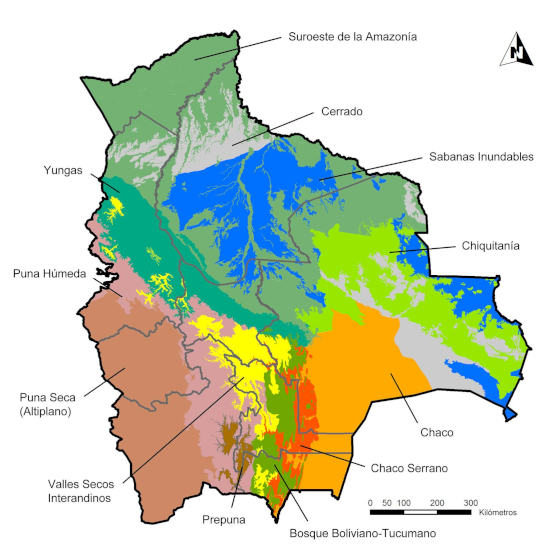
\includegraphics[width=0.72\textwidth]{img/mapa_ecorregiones_bolivia.png}
  \caption{Ecorregiones principales de Bolivia. La variedad de biomas ---desde los llanos
           amazónicos hasta el Altiplano y los Yungas andinos--- explica la extraordinaria
           riqueza de aves y mamíferos del país.}
  \label{fig:ecorregiones}
\end{figure}

En este contexto, la ausencia de evaluación de riesgo para el 11,8\,\% de las especies de aves
y mamíferos bolivianos no es un problema académico menor: es una laguna crítica en la base
de conocimiento necesaria para priorizar acciones de conservación en uno de los países
con mayor velocidad de pérdida de hábitat de América del Sur.

\subsection{Aprendizaje automático aplicado a conservación}

La intersección entre aprendizaje automático y biología de la conservación ha experimentado
un crecimiento sostenido en la última década.
La premisa fundamental es que las categorías IUCN, aunque asignadas mediante criterios expertos,
correlacionan con rasgos biológicos y ambientales mesurables, lo que las hace ---al menos
parcialmente--- predecibles mediante clasificadores supervisados.

\paragraph{Antecedentes directos.}
Bland et al.\ (2015) \cite{bland2015} entrenaron árboles de decisión con rasgos morfológicos
y ecológicos de peces dulceacuícolas para predecir su categoría IUCN, obteniendo una exactitud
del 72\,\% y demostrando que la masa corporal y el tamaño del área de distribución son los
predictores más robustos.
Lee \& Jetz (2011) \cite{lee2017} aplicaron Random Forest a aves de distribución global,
alcanzando un AUC de 0,81 y concluyendo que el tamaño del rango geográfico domina sobre
las variables climáticas para la mayoría de las aves.
Szabo et al.\ (2012) \cite{szabo2012} analizaron patrones globales de extinción de aves
a nivel de subespecie, identificando que la especialización de hábitat y el tamaño corporal
son factores predictivos clave incluso a escalas taxonómicas finas.

\paragraph{Tendencias recientes.}
Trabajos más recientes han incorporado datos de teledetección (NDVI, pérdida forestal,
expansión agrícola) y datos de presencia masiva de plataformas ciudadanas como GBIF e iNaturalist.
Cardillo et al.\ (2005) \cite{cardillo2004} identificaron que en mamíferos la combinación
de rasgos intrínsecos (masa corporal, tasa reproductiva) con presiones externas (densidad
humana) supera en poder predictivo a cualquiera de los dos grupos por separado.
La adopción de Gradient Boosting y métodos de ensamble ha mejorado consistentemente los
resultados respecto a clasificadores más simples, aunque a costa de mayor complejidad interpretativa.

\paragraph{Vacíos en la región andino-amazónica.}
A pesar de estos avances globales, existe una brecha notable en estudios centrados en
Bolivia o en la región andino-amazónica en general.
La mayoría de los trabajos citados utilizan distribuciones globales de especies con miles
de observaciones por especie; Bolivia presenta el reto adicional de tener registros GBIF
muy desbalanceados (pocas ocurrencias para muchas especies raras) y una fracción significativa
de sus especies sin evaluación IUCN.
El presente proyecto aporta una metodología adaptada a estas condiciones, incorporando
específicamente capas de presión humana de RAISG (minería ilegal, bloques petroleros, quemas
y vialidad) que no han sido empleadas en estudios anteriores para esta región.

\subsection{Bases de datos empleadas}

\paragraph{GBIF.} El \textit{Global Biodiversity Information Facility} centraliza más de 2\,000
millones de registros de ocurrencia de especies a escala global.
Para este proyecto se descargaron 1\,37 millones de registros de Bolivia (2000--2024).

\paragraph{AVONET.} Base de datos de rasgos morfológicos y ecológicos de 11\,009 especies de aves
\cite{tobias2022avonet}, con variables como masa corporal, longitud de ala y nivel trófico.

\paragraph{PanTHERIA.} Base de datos de rasgos de vida de 5\,416 especies de mamíferos
\cite{jones2009pantheria}, con variables como masa corporal adulta y ciclo de actividad.

\paragraph{WorldClim v2.1.} Datos climáticos globales a 1 km de resolución espacial \cite{fick2017worldclim},
derivados de estaciones meteorológicas para el período 1970--2000.

\paragraph{Global Forest Watch.} Producto de detección satelital de pérdida de cubierta arbórea
a resolución de 30 m, año a año desde 2001 \cite{hansen2013gfw}.

\paragraph{MapBiomas Amazonia.} Clasificación anual de cobertura y uso del suelo de la Amazonia
boliviana a partir de imágenes Landsat, con 14 clases temáticas.

\paragraph{RAISG.} La \textit{Red Amazónica de Información Socioambiental Georeferenciada} provee
shapefiles de áreas naturales protegidas (ANP), territorios indígenas (TI), concesiones mineras,
bloques petroleros, vías y quemas de la Amazonia boliviana.

%===============================================================
\section{Problemática}
%===============================================================

\subsection{Descripción del problema}

De las 1\,718 especies de aves y mamíferos registradas en Bolivia en GBIF,
\textbf{202 no cuentan con evaluación IUCN}.  Esto representa el 11,8\,\% del total.
Adicionalmente, 14 mamíferos clasificados como DD (Datos Insuficientes) no pueden
incorporarse al análisis supervisado por carecer de etiqueta fiable.

Sin una evaluación cuantitativa del riesgo, las decisiones de conservación ---qué
especies proteger, en qué zonas ampliar ANPs, qué actividades extractivas restringir---
carecen de fundamento técnico para estas 202 especies.

El problema central no es la ausencia de datos per se: existen registros de ocurrencia
para la mayoría de esas especies en GBIF, así como información climática y de presión
humana disponible públicamente.  El problema es la \textbf{ausencia de metodología aplicada}
que integre esas fuentes para producir una estimación probabilística de riesgo.

\subsection{Árbol de problemas}

\begin{figure}[H]
\centering
\resizebox{\textwidth}{!}{%
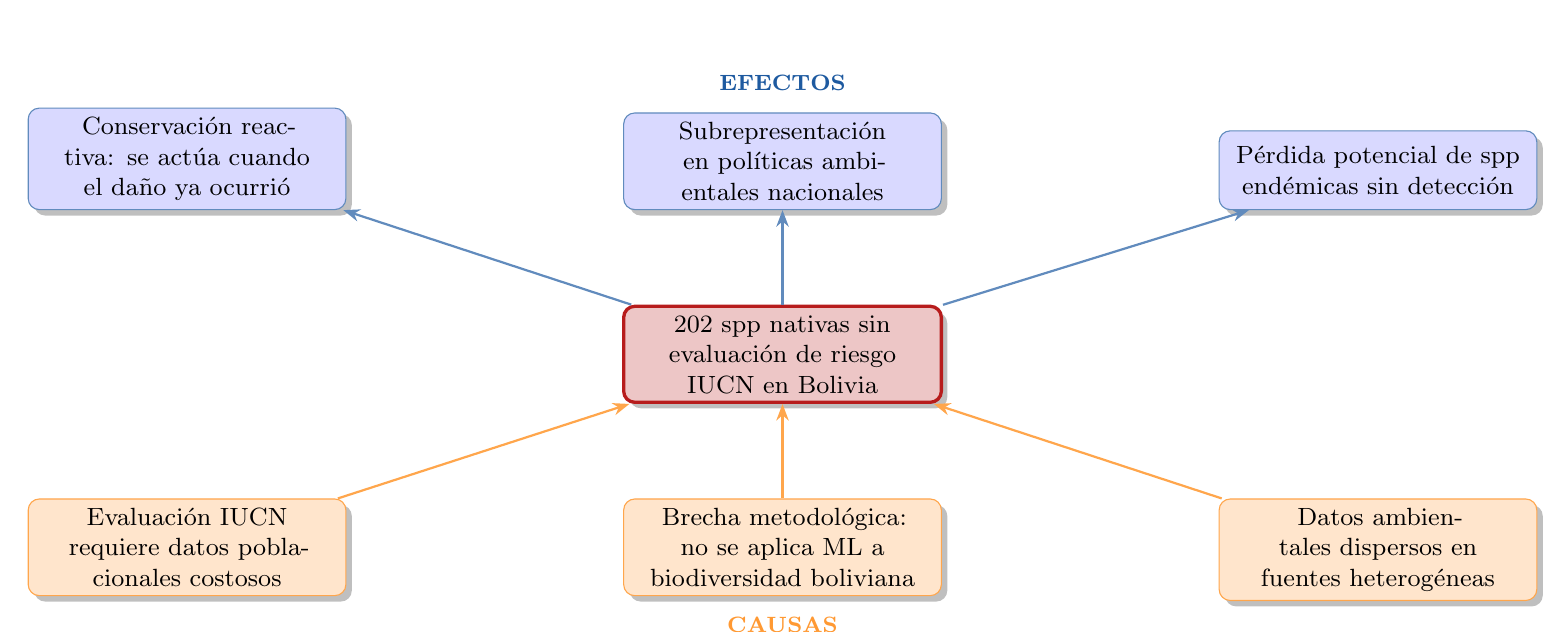
\begin{tikzpicture}[
  node distance=0.7cm and 1.2cm,
  box/.style={rectangle, rounded corners=4pt, draw, fill=white,
              text width=3.8cm, align=center, font=\small,
              drop shadow, minimum height=1cm},
  prob/.style={box, fill=rojoBio!25, draw=rojoBio, line width=1.2pt},
  causa/.style={box, fill=orange!20, draw=orange!70},
  efecto/.style={box, fill=blue!15, draw=azulBio!70},
  arrow/.style={-{Stealth[length=6pt]}, thick}
]
% Problema central
\node[prob] (centro) {202 spp nativas sin evaluación de riesgo IUCN en Bolivia};

% CAUSAS (debajo)
\node[causa, below left=1.2cm and 3.5cm of centro]  (c1) {Evaluación IUCN requiere datos poblacionales costosos};
\node[causa, below=1.2cm of centro]                 (c2) {Brecha metodológica: no se aplica ML a biodiversidad boliviana};
\node[causa, below right=1.2cm and 3.5cm of centro] (c3) {Datos ambientales dispersos en fuentes heterogéneas};

% EFECTOS (arriba)
\node[efecto, above left=1.2cm and 3.5cm of centro]  (e1) {Conservación reactiva: se actúa cuando el daño ya ocurrió};
\node[efecto, above=1.2cm of centro]                  (e2) {Subrepresentación en políticas ambientales nacionales};
\node[efecto, above right=1.2cm and 3.5cm of centro] (e3) {Pérdida potencial de spp endémicas sin detección};

% Flechas causas→problema
\draw[arrow, orange!70] (c1) -- (centro);
\draw[arrow, orange!70] (c2) -- (centro);
\draw[arrow, orange!70] (c3) -- (centro);

% Flechas problema→efectos
\draw[arrow, azulBio!70] (centro) -- (e1);
\draw[arrow, azulBio!70] (centro) -- (e2);
\draw[arrow, azulBio!70] (centro) -- (e3);

% Etiquetas
\node[font=\footnotesize\bfseries, color=orange!80, below=0.15cm of c2] {CAUSAS};
\node[font=\footnotesize\bfseries, color=azulBio,   above=0.15cm of e2] {EFECTOS};

\end{tikzpicture}%
}% fin resizebox
\caption{Árbol de problemas del proyecto BioAlerta.}
\label{fig:arbol_problemas}
\end{figure}

%===============================================================
\section{Objetivo}
%===============================================================

\subsection{Objetivo general}

Desarrollar un modelo de aprendizaje automático supervisado que prediga el estatus de amenaza
de extinción (amenazada / no amenazada) de especies nativas de Bolivia a partir de factores
ambientales, geoespaciales y biológicos, y que genere predicciones probabilísticas para las
202 especies sin evaluación IUCN.

\subsection{Objetivos específicos}

\begin{enumerate}[label=\textbf{OE\arabic*.}]
  \item Construir un \textit{dataset} integrado que combine registros de ocurrencia GBIF,
        variables bioclimáticas WorldClim, datos de deforestación GFW, cobertura del suelo
        MapBiomas, presiones humanas RAISG y rasgos biológicos AVONET/PanTHERIA.
  \item Realizar un análisis exploratorio de datos que identifique los patrones de correlación
        entre las variables del dataset y el estado de amenaza de cada especie.
  \item Comparar el desempeño de cinco algoritmos de clasificación supervisada ---Regresión Logística,
        Random Forest, Gradient Boosting, SVM y KNN--- mediante validación cruzada estratificada
        con métricas robustas al desbalance de clases.
  \item Identificar las variables con mayor peso predictivo mediante análisis de importancia de
        características del mejor modelo.
  \item Generar predicciones probabilísticas de amenaza para las 202 especies sin evaluación IUCN
        como insumo para decisiones de conservación.
\end{enumerate}

\subsection{Árbol de objetivos}

\begin{figure}[H]
\centering
\resizebox{\textwidth}{!}{%
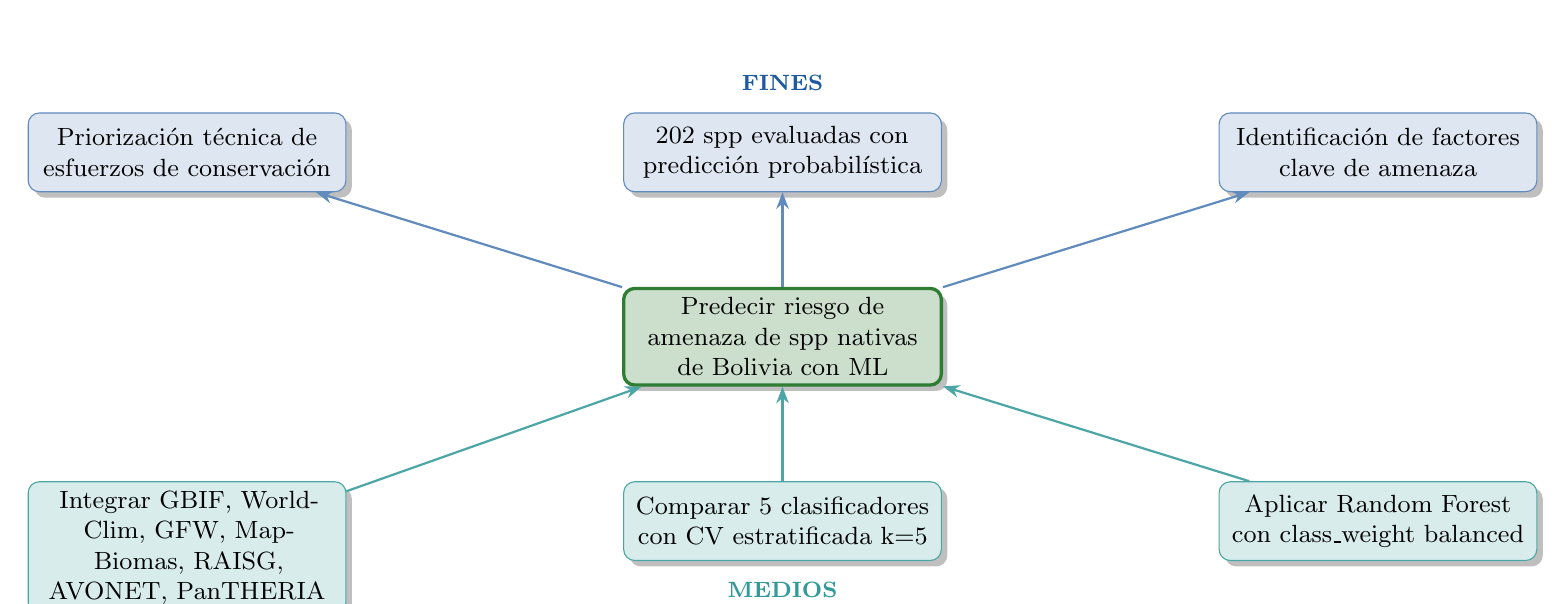
\begin{tikzpicture}[
  node distance=0.7cm and 1.2cm,
  box/.style={rectangle, rounded corners=4pt, draw, fill=white,
              text width=3.8cm, align=center, font=\small,
              drop shadow, minimum height=1cm},
  obj/.style={box, fill=verdeBio!25, draw=verdeBio, line width=1.2pt},
  medio/.style={box, fill=teal!15, draw=teal!70},
  fin/.style={box, fill=azulBio!15, draw=azulBio!70},
  arrow/.style={-{Stealth[length=6pt]}, thick}
]
% Objetivo central
\node[obj] (centro) {Predecir riesgo de amenaza de spp nativas de Bolivia con ML};

% MEDIOS (abajo)
\node[medio, below left=1.2cm and 3.5cm of centro]  (m1) {Integrar GBIF, WorldClim, GFW, MapBiomas, RAISG, AVONET, PanTHERIA};
\node[medio, below=1.2cm of centro]                 (m2) {Comparar 5 clasificadores con CV estratificada k=5};
\node[medio, below right=1.2cm and 3.5cm of centro] (m3) {Aplicar Random Forest con class\_weight balanced};

% FINES (arriba)
\node[fin, above left=1.2cm and 3.5cm of centro]  (f1) {Priorización técnica de esfuerzos de conservación};
\node[fin, above=1.2cm of centro]                  (f2) {202 spp evaluadas con predicción probabilística};
\node[fin, above right=1.2cm and 3.5cm of centro] (f3) {Identificación de factores clave de amenaza};

% Flechas medios→objetivo
\draw[arrow, teal!70]    (m1) -- (centro);
\draw[arrow, teal!70]    (m2) -- (centro);
\draw[arrow, teal!70]    (m3) -- (centro);

% Flechas objetivo→fines
\draw[arrow, azulBio!70] (centro) -- (f1);
\draw[arrow, azulBio!70] (centro) -- (f2);
\draw[arrow, azulBio!70] (centro) -- (f3);

% Etiquetas
\node[font=\footnotesize\bfseries, color=teal!80,   below=0.15cm of m2] {MEDIOS};
\node[font=\footnotesize\bfseries, color=azulBio,   above=0.15cm of f2] {FINES};

\end{tikzpicture}%
}% fin resizebox
\caption{Árbol de objetivos del proyecto BioAlerta.}
\label{fig:arbol_objetivos}
\end{figure}

%===============================================================
\section{Justificación}
%===============================================================

\subsection{Justificación social}

Bolivia posee una de las mayores extensiones de bosques tropicales en América del Sur y su
biodiversidad sustenta modos de vida de decenas de pueblos indígenas y comunidades campesinas.
La pérdida de especies tiene efectos directos sobre servicios ecosistémicos como la regulación
del agua, la polinización de cultivos y el control de plagas.
BioAlerta genera información accionable para el Ministerio de Medio Ambiente y Agua (MMAyA),
ONGs de conservación y municipios, permitiéndoles focalizar recursos donde el riesgo es mayor
pero no documentado.

\subsection{Justificación académica}

En el ámbito de la bioinformática y ecología computacional, la aplicación de ML a datos
de ocurrencia y rasgos biológicos es un campo activo pero con escasa presencia de estudios
centrados en Bolivia o en la región andino-amazónica.
Este trabajo aporta una metodología replicable, un \textit{pipeline} reproducible en Python
y resultados cuantitativos que pueden servir de línea base para estudios posteriores a mayor
resolución espacial o temporal.

\subsection{Justificación técnica}

El proyecto demuestra la viabilidad de integrar fuentes de datos heterogéneas ---vectoriales,
raster y tabulares--- en un flujo de procesamiento automatizado mediante herramientas de código
abierto: GBIF/pygbif para descarga, rasterio y geopandas para extracción espacial, y
scikit-learn para modelado.
La totalidad del código está estructurada en Jupyter Notebooks numerados (01--06) que pueden
ejecutarse de forma reproducible en el entorno conda \texttt{bioalerta}.

\subsection{Justificación científica}

La identificación de los factores predictores más importantes ---en especial la prevalencia
de rasgos biológicos sobre variables ambientales--- arroja luz sobre los mecanismos subyacentes
a la vulnerabilidad de las especies.
Este hallazgo es consistente con la literatura ecológica que señala que especies de mayor masa
corporal, menor tamaño de rango geográfico y nichos tróficos especializados son
intrínsecamente más vulnerables a perturbaciones, independientemente del contexto ambiental
inmediato.

%===============================================================
\section{Metodología}
%===============================================================

El proyecto sigue el modelo \textbf{CRISP-DM} (\textit{Cross-Industry Standard Process for
Data Mining}), ampliamente adoptado en proyectos de ciencia de datos, complementado con
elementos del modelo \textbf{KDD} (\textit{Knowledge Discovery in Databases}).

\subsection{Fases CRISP-DM aplicadas al proyecto}

\begin{enumerate}[label=\textbf{Fase \arabic*:}]
  \item \textbf{Comprensión del negocio / dominio.}
        Definición del objetivo de conservación: predecir amenaza como clasificación binaria
        (threatened/not threatened) usando la codificación IUCN.
        Decisión de construir modelos separados para aves y mamíferos dado que tienen
        distintas fuentes de rasgos y distribuciones de clase diferentes.

  \item \textbf{Comprensión de los datos.}
        Exploración de GBIF (1,37M registros), validación de cobertura temporal (2000--2024),
        mapeo de categorías IUCN por especie vía Wikidata SPARQL, evaluación de completitud
        en AVONET (89,1\,\% de coincidencia para aves) y PanTHERIA (81,2\,\% para mamíferos).

  \item \textbf{Preparación de los datos.}
        Extracción espacial (notebook 03), construcción de \textit{features} (notebook 04):
        limpieza de nodata en variables bioclimáticas, imputación con medianas/modas del
        conjunto de entrenamiento, \textit{one-hot encoding} de variables categóricas AVONET.

  \item \textbf{Modelado.}
        Comparación de cinco clasificadores con validación cruzada estratificada (notebook 06).
        Selección del mejor modelo por ROC-AUC promedio.

  \item \textbf{Evaluación.}
        Análisis de importancia de variables, interpretación biológica de resultados,
        predicción para las 202 especies sin IUCN.

  \item \textbf{Despliegue.}
        Exportación de predicciones a \texttt{predicciones.parquet}.
        Trabajo futuro: visualización web interactiva con mapa de Bolivia (GeoJSON/JSON estáticos).
\end{enumerate}

\subsection{Diagrama del pipeline}

\begin{figure}[H]
\centering
\resizebox{\textwidth}{!}{%
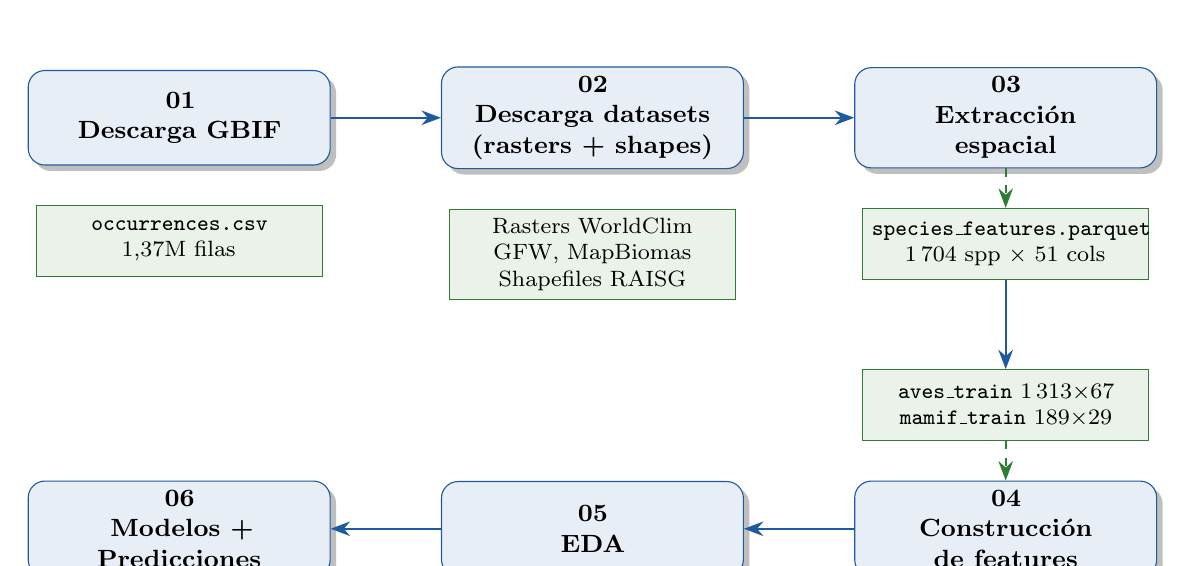
\begin{tikzpicture}[
  proc/.style={rectangle, rounded corners=6pt, draw=azulBio, fill=azulBio!10,
               text width=3.6cm, align=center, font=\small\bfseries,
               minimum height=1.2cm, drop shadow},
  data/.style={rectangle, draw=verdeBio, fill=verdeBio!10,
               text width=3.4cm, align=center, font=\footnotesize,
               minimum height=0.9cm},
  arrow/.style={-{Stealth[length=7pt]}, thick, color=azulBio},
  node distance=0.6cm and 1.4cm
]

% Fila superior: notebooks 01-02-03
\node[proc] (nb01) {01\\ Descarga GBIF};
\node[proc, right=1.4cm of nb01] (nb02) {02\\ Descarga datasets\\(rasters + shapes)};
\node[proc, right=1.4cm of nb02] (nb03) {03\\ Extracción\\espacial};

% Fila inferior: notebooks 06-05-04 (de izquierda a derecha)
\node[proc, below=4.0cm of nb01] (nb06) {06\\ Modelos +\\Predicciones};
\node[proc, right=1.4cm of nb06] (nb05) {05\\ EDA};
\node[proc, right=1.4cm of nb05] (nb04) {04\\ Construcción\\de features};

% Datos intermedios fila superior
\node[data, below=0.5cm of nb01] (gbif)    {\texttt{occurrences.csv}\\1{,}37M filas};
\node[data, below=0.5cm of nb02] (rasters) {Rasters WorldClim\\GFW, MapBiomas\\Shapefiles RAISG};

% Datos intermedios columna derecha (entre nb03 y nb04)
\node[data, below=0.5cm of nb03] (parq1)   {\texttt{species\_features.parquet}\\1\,704 spp $\times$ 51 cols};
\node[data, above=0.5cm of nb04] (parq2)   {\texttt{aves\_train} 1\,313$\times$67\\\texttt{mamif\_train} 189$\times$29};

% Flechas fila superior
\draw[arrow] (nb01) -- (nb02);
\draw[arrow] (nb02) -- (nb03);

% Flecha nb03 → nb04 (bajando por la derecha)
\draw[arrow] (parq1.south) -- (parq2.north);

% Flechas fila inferior (derecha a izquierda)
\draw[arrow] (nb04) -- (nb05);
\draw[arrow] (nb05) -- (nb06);

% Conexiones de datos con notebooks
\draw[arrow, verdeBio, dashed] (nb03.south) -- (parq1.north);
\draw[arrow, verdeBio, dashed] (parq2.south) -- (nb04.north);

\end{tikzpicture}%
}% fin resizebox
\caption{Pipeline de procesamiento del proyecto BioAlerta (notebooks 01--06).
         Las cajas azules son notebooks; las verdes son artefactos de datos intermedios.}
\label{fig:pipeline}
\end{figure}

\subsection{Diseño del estudio}

\paragraph{Variable objetivo.}
Se define una variable binaria \texttt{threatened}: las categorías VU, EN y CR se codifican
como 1 (amenazada); LC y NT como 0 (no amenazada).
Las categorías DD y las especies sin evaluación IUCN se excluyen del entrenamiento
y las últimas se usan como conjunto de predicción.

\paragraph{Modelos separados por clase taxonómica.}
Se construyen modelos independientes para aves y mamíferos porque: (1) los conjuntos de
rasgos biológicos provienen de fuentes distintas; (2) los índices de desbalance difieren
(1:35 para aves y 1:14 para mamíferos); (3) los patrones ecológicos de vulnerabilidad
pueden ser distintos entre clases.

\paragraph{Manejo del desbalance.}
Se aplica \verb|class_weight='balanced'| en todos los clasificadores que lo admiten
(LR, RF, GB, SVM), lo que pondera las pérdidas inversamente proporcional a la frecuencia
de cada clase.
Se evita \textit{accuracy} como métrica principal y se prioriza ROC-AUC, PR-AUC y
F1-macro, que son robustos al desbalance.

%===============================================================
\section{Desarrollo}
%===============================================================

\subsection{Recopilación y preparación de datos}

\subsubsection{Registros de ocurrencia (GBIF)}

Se descargaron registros de presencia para todas las aves y mamíferos de Bolivia del portal
GBIF mediante la librería \texttt{pygbif}, filtrando por:
\begin{itemize}[nosep]
  \item País: Bolivia (código \texttt{BO})
  \item Período: 2000--2024
  \item Coordenadas geográficas válidas (no nulas)
  \item Clase taxonómica: Aves o Mammalia
\end{itemize}

El resultado fue \textbf{1\,37 millones de registros} cubriendo \textbf{1\,718 especies}
(1\,478 aves y 240 mamíferos).  Cada registro contiene: identificador, clase, orden, familia,
género, especie, latitud/longitud decimal, provincia, fecha y tipo de registro.

\subsubsection{Categorías IUCN}

La IUCN no dispone de API pública de libre acceso, por lo que las categorías se obtuvieron
mediante consultas SPARQL a \textbf{Wikidata}, que agrega información de la Lista Roja.
Se construyeron tablas separadas para aves (\texttt{iucn\_aves.csv}, 1\,478 spp) y mamíferos
(\texttt{iucn\_mamiferos.csv}, 240 spp).

De la unión con GBIF se obtienen los conjuntos finales con etiqueta:
\begin{itemize}[nosep]
  \item \textbf{Aves:} 1\,313 spp con IUCN válida (LC/NT/VU/EN/CR) $+$ 165 spp sin IUCN
  \item \textbf{Mamíferos:} 189 spp con IUCN válida $+$ 37 spp sin IUCN $+$ 14 spp DD (excluidas)
\end{itemize}

\subsubsection{Rasgos biológicos}

\paragraph{AVONET (aves).}
La base AVONET \cite{tobias2022avonet} cubre 11\,009 especies de aves con 15 variables morfológicas
y ecológicas.  Se seleccionó un subconjunto (\textit{slim}) con las columnas de mayor relevancia
ecológica (tabla~\ref{tab:avonet}).  La tasa de coincidencia con las aves bolivianas de GBIF fue
del \textbf{89,1\,\%}.

\begin{table}[H]
  \centering\small
  \caption{Variables AVONET incluidas en el dataset.}
  \label{tab:avonet}
  \begin{tabular}{lll}
    \toprule
    \textbf{Variable} & \textbf{Tipo} & \textbf{Descripción} \\
    \midrule
    Mass              & Numérica   & Masa corporal (g) \\
    Beak.Length\_Culmen & Numérica & Longitud del pico (mm) \\
    Beak.Width        & Numérica   & Ancho del pico (mm) \\
    Beak.Depth        & Numérica   & Profundidad del pico (mm) \\
    Tarsus.Length     & Numérica   & Longitud del tarso (mm) \\
    Wing.Length       & Numérica   & Longitud del ala (mm) \\
    Kipps.Distance    & Numérica   & Índice de forma del ala \\
    Range.Size        & Numérica   & Tamaño del rango geográfico (km²) \\
    Habitat           & Categórica & Tipo de hábitat principal \\
    Migration         & Categórica & Patrón migratorio (1=sedentario, 3=migratorio) \\
    Trophic.Level     & Categórica & Nivel trófico \\
    Trophic.Niche     & Categórica & Nicho trófico detallado \\
    Primary.Lifestyle & Categórica & Estilo de vida principal \\
    Habitat.Density   & Numérica   & Densidad del hábitat preferido \\
    \bottomrule
  \end{tabular}
\end{table}

\paragraph{PanTHERIA (mamíferos).}
La base PanTHERIA \cite{jones2009pantheria} cubre 5\,416 especies con 56 variables de historia
de vida, pero más del 75\,\% de las columnas presentan valores nulos en las especies bolivianas.
Se retuvieron únicamente las 4 variables con cobertura razonable:
\texttt{AdultBodyMass\_g}, \texttt{TrophicLevel}, \texttt{GR\_Area\_km2} y \texttt{ActivityCycle}.
La tasa de coincidencia con mamíferos bolivianos fue del \textbf{81,2\,\%}.

\subsection{Fundamentos de datos geoespaciales}

Para comprender cómo se construyen las variables ambientales del dataset es necesario
entender los dos tipos de datos geoespaciales empleados en este proyecto: datos
\textbf{raster} y datos \textbf{vectoriales}.

\subsubsection{¿Qué es un raster?}

Un \textbf{raster} es una estructura de datos geoespaciales que representa el espacio
como una \textbf{cuadrícula regular de celdas} (píxeles), donde cada celda almacena
un valor numérico asociado a esa porción del territorio.
Es conceptualmente idéntico a una imagen digital, pero con la diferencia de que cada
píxel tiene coordenadas geográficas reales.

\begin{figure}[H]
\centering
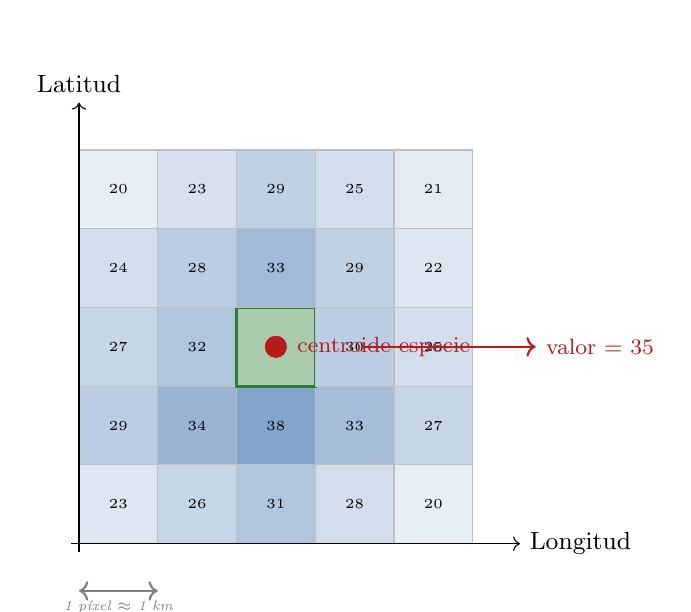
\begin{tikzpicture}[scale=1.0]
  % Fila 0
  \draw[fill=azulBio!15,draw=gray!50] (0,0) rectangle (1,1); \node[font=\tiny] at (0.5,0.5) {23};
  \draw[fill=azulBio!25,draw=gray!50] (1,0) rectangle (2,1); \node[font=\tiny] at (1.5,0.5) {26};
  \draw[fill=azulBio!35,draw=gray!50] (2,0) rectangle (3,1); \node[font=\tiny] at (2.5,0.5) {31};
  \draw[fill=azulBio!20,draw=gray!50] (3,0) rectangle (4,1); \node[font=\tiny] at (3.5,0.5) {28};
  \draw[fill=azulBio!10,draw=gray!50] (4,0) rectangle (5,1); \node[font=\tiny] at (4.5,0.5) {20};
  % Fila 1
  \draw[fill=azulBio!30,draw=gray!50] (0,1) rectangle (1,2); \node[font=\tiny] at (0.5,1.5) {29};
  \draw[fill=azulBio!45,draw=gray!50] (1,1) rectangle (2,2); \node[font=\tiny] at (1.5,1.5) {34};
  \draw[fill=azulBio!55,draw=gray!50] (2,1) rectangle (3,2); \node[font=\tiny] at (2.5,1.5) {38};
  \draw[fill=azulBio!40,draw=gray!50] (3,1) rectangle (4,2); \node[font=\tiny] at (3.5,1.5) {33};
  \draw[fill=azulBio!25,draw=gray!50] (4,1) rectangle (5,2); \node[font=\tiny] at (4.5,1.5) {27};
  % Fila 2 (resaltada)
  \draw[fill=azulBio!25,draw=gray!50] (0,2) rectangle (1,3); \node[font=\tiny] at (0.5,2.5) {27};
  \draw[fill=azulBio!35,draw=gray!50] (1,2) rectangle (2,3); \node[font=\tiny] at (1.5,2.5) {32};
  \draw[fill=verdeBio!40,draw=verdeBio,line width=1.2pt] (2,2) rectangle (3,3);
    \node[font=\tiny\bfseries] at (2.5,2.5) {35};
  \draw[fill=azulBio!30,draw=gray!50] (3,2) rectangle (4,3); \node[font=\tiny] at (3.5,2.5) {30};
  \draw[fill=azulBio!20,draw=gray!50] (4,2) rectangle (5,3); \node[font=\tiny] at (4.5,2.5) {25};
  % Fila 3
  \draw[fill=azulBio!20,draw=gray!50] (0,3) rectangle (1,4); \node[font=\tiny] at (0.5,3.5) {24};
  \draw[fill=azulBio!30,draw=gray!50] (1,3) rectangle (2,4); \node[font=\tiny] at (1.5,3.5) {28};
  \draw[fill=azulBio!42,draw=gray!50] (2,3) rectangle (3,4); \node[font=\tiny] at (2.5,3.5) {33};
  \draw[fill=azulBio!28,draw=gray!50] (3,3) rectangle (4,4); \node[font=\tiny] at (3.5,3.5) {29};
  \draw[fill=azulBio!15,draw=gray!50] (4,3) rectangle (5,4); \node[font=\tiny] at (4.5,3.5) {22};
  % Fila 4
  \draw[fill=azulBio!10,draw=gray!50] (0,4) rectangle (1,5); \node[font=\tiny] at (0.5,4.5) {20};
  \draw[fill=azulBio!18,draw=gray!50] (1,4) rectangle (2,5); \node[font=\tiny] at (1.5,4.5) {23};
  \draw[fill=azulBio!28,draw=gray!50] (2,4) rectangle (3,5); \node[font=\tiny] at (2.5,4.5) {29};
  \draw[fill=azulBio!20,draw=gray!50] (3,4) rectangle (4,5); \node[font=\tiny] at (3.5,4.5) {25};
  \draw[fill=azulBio!12,draw=gray!50] (4,4) rectangle (5,5); \node[font=\tiny] at (4.5,4.5) {21};
  % Ejes
  \draw[->] (-0.1,0) -- (5.6,0) node[right,font=\small] {Longitud};
  \draw[->] (0,-0.1) -- (0,5.6) node[above,font=\small] {Latitud};
  % Punto de muestreo
  \fill[rojoBio] (2.5,2.5) circle (4pt);
  \node[font=\footnotesize, rojoBio, right=0.15cm] at (2.5,2.5) {centroide especie};
  \draw[->, rojoBio, thick] (3.6,2.5) -- (5.8,2.5)
    node[right,font=\footnotesize,rojoBio] {valor = 35};
  % Leyenda tamano pixel
  \draw[<->, gray, thick] (0,-0.6) -- (1,-0.6)
    node[midway, below, font=\tiny\itshape] {1 píxel $\approx$ 1 km};
\end{tikzpicture}
\caption{Representación esquemática de un raster. Cada celda almacena un valor numérico
         (aquí: temperatura $\times 10$). El punto rojo es el centroide de una especie;
         la celda resaltada en verde es la que se muestrea con \texttt{rasterio.sample}.}
\label{fig:raster_esquema}
\end{figure}

Las propiedades fundamentales de un raster son:

\begin{itemize}
  \item \textbf{Resolución espacial:} el tamaño real de cada píxel sobre el terreno.
        Por ejemplo, WorldClim tiene resolución de $\approx$1 km, lo que significa que
        cada celda representa un área de 1 km $\times$ 1 km.
        GFW tiene resolución de 30 m (imágenes Landsat).

  \item \textbf{Sistema de referencia de coordenadas (CRS):} el marco matemático que
        define cómo se proyectan las coordenadas esféricas de la Tierra sobre un plano
        2D.  En este proyecto se utilizan dos:
        \begin{itemize}[nosep]
          \item \textbf{EPSG:4326} (WGS84 geográfico): coordenadas en grados decimales
                de latitud y longitud.  Todos los rasters se almacenan en este sistema.
          \item \textbf{EPSG:32720} (UTM zona 20S): sistema proyectado métrico para la
                región de Bolivia.  Se usa para calcular distancias en kilómetros, ya
                que en EPSG:4326 un grado de longitud no equivale a la misma distancia
                en todas las latitudes.
        \end{itemize}

  \item \textbf{Valor nodata:} las celdas fuera del área de cobertura del raster
        (por ejemplo, píxeles oceánicos en un raster continental) se marcan con un
        valor centinela especial denominado \texttt{nodata}.  Para WorldClim este valor
        es $-32768$ o valores de orden $10^{35}$, que deben detectarse y descartarse
        antes del análisis.

  \item \textbf{Bandas:} un raster puede tener una o más bandas, análogas a los canales
        de color de una imagen.  Cada banda almacena una variable diferente en la misma
        cuadrícula.  En este proyecto, cada variable bioclimática de WorldClim es un
        archivo GeoTIFF separado de una sola banda.
\end{itemize}

\subsubsection{Formato GeoTIFF}

Los rasters de este proyecto se almacenan en formato \textbf{GeoTIFF} (\texttt{.tif}),
que es el estándar de facto en teledetección y análisis geoespacial.
Un GeoTIFF es una imagen TIFF estándar con metadatos georreferenciados incrustados:
las coordenadas de la esquina superior izquierda, el tamaño del píxel en unidades del
CRS, el CRS mismo y la matriz de transformación afín que convierte filas/columnas de
píxel en coordenadas geográficas.

La librería \textbf{rasterio} (Python) permite leer GeoTIFFs y expone esta información
como el objeto \texttt{transform} (la transformación afín) y \texttt{crs} (el sistema
de referencia).  Su función \texttt{rasterio.sample(coords)} recibe una lista de
coordenadas $(lon, lat)$ y devuelve, para cada punto, el valor del píxel más cercano
---sin necesidad de cargar todo el raster en memoria.

\begin{samepage}
\begin{lstlisting}[caption={Extracción de valores raster con rasterio.sample.}]
import rasterio
import numpy as np

with rasterio.open('data/worldclim/bio1_bolivia.tif') as src:
    # coords: lista de (longitud, latitud) de cada especie
    coords = list(zip(df['lon_centroid'], df['lat_centroid']))
    # sample devuelve un generador de arrays de 1 valor por punto
    values = [v[0] for v in src.sample(coords)]
    df['bio1_mean'] = values
\end{lstlisting}
\end{samepage}

\subsubsection{Datos vectoriales y la librería GeoPandas}

A diferencia de los rasters, los \textbf{datos vectoriales} representan el espacio
mediante \textbf{geometrías} (puntos, líneas y polígonos) con atributos asociados.
Son el equivalente geoespacial de una tabla de base de datos donde cada fila tiene una
forma geométrica en lugar de solo números.

En este proyecto los datos vectoriales provienen de RAISG y se almacenan en formato
\textbf{Shapefile} (\texttt{.shp}) y \textbf{GeoJSON}.
La librería \textbf{GeoPandas} extiende pandas con un tipo de columna especial
\texttt{geometry} que almacena estas formas y permite operaciones espaciales como:

\begin{itemize}[nosep]
  \item \texttt{sjoin(within)}: determina si cada punto de ocurrencia cae dentro de un
        polígono (p.ej.\ dentro de un ANP).
  \item \texttt{sjoin\_nearest}: encuentra el polígono más cercano a cada punto y
        devuelve la distancia.  Requiere CRS proyectado (EPSG:32720) para que la
        distancia sea en metros, no en grados.
\end{itemize}

\begin{samepage}
\begin{lstlisting}[caption={Operación espacial: porcentaje de ocurrencias dentro de ANPs.}]
import geopandas as gpd

# Puntos de ocurrencia como GeoDataFrame
gdf_occ = gpd.GeoDataFrame(df_occ,
    geometry=gpd.points_from_xy(df_occ.lon, df_occ.lat),
    crs='EPSG:4326')

# Poligonos de ANPs
gdf_anp = gpd.read_file('data/raisg/Anps_jun2025/ANP_nacional.shp')
gdf_anp = gdf_anp.to_crs('EPSG:4326')

# Containment: cuantos puntos de cada especie caen dentro de un ANP
joined = gpd.sjoin(gdf_occ, gdf_anp, how='left', predicate='within')
pct_anp = joined.groupby('species')['index_right'].apply(
    lambda x: x.notna().mean())  # fraccion de puntos dentro
\end{lstlisting}
\end{samepage}

\subsubsection{Recorte a Bolivia (gdalwarp)}

Los rasters globales de WorldClim, GFW y MapBiomas se descargaron a nivel mundial o
regional y se recortaron al territorio boliviano usando la herramienta \texttt{gdalwarp}
de la suite GDAL (Geospatial Data Abstraction Library):

\begin{lstlisting}[caption={Recorte de raster a Bolivia con gdalwarp.},language=bash]
gdalwarp -cutline bolivia.shp -crop_to_cutline \
         -t_srs EPSG:4326 input_global.tif output_bolivia.tif
\end{lstlisting}

Este recorte reduce el tamaño de los archivos de varios GB a decenas de MB,
acelerando todas las operaciones de extracción posteriores.

\subsection{Extracción espacial de variables (Notebook 03)}

\subsubsection{Centroide de especie}

Para cada especie se calculó el \textbf{centroide geográfico} como la mediana de las latitudes
y longitudes de todos sus registros de ocurrencia.  El uso de la mediana en lugar de la media
hace al centroide robusto frente a registros erróneos con coordenadas extremas.

\subsubsection{Variables raster}

Para cada centroide se extrajeron valores de los rasters mediante \texttt{rasterio.sample}
(muestreo puntual vectorizado, mucho más rápido que la alternativa \texttt{rasterstats}).

\paragraph{WorldClim v2.1.}
Se emplearon 6 de las 19 variables bioclimáticas disponibles (tabla~\ref{tab:worldclim}),
recortadas a Bolivia en proyección EPSG:4326.

\begin{table}[H]
  \centering\small
  \caption{Variables bioclimáticas WorldClim v2.1 seleccionadas.}
  \label{tab:worldclim}
  \begin{tabular}{lll}
    \toprule
    \textbf{Variable} & \textbf{Descripción} & \textbf{Unidades} \\
    \midrule
    BIO1  & Temperatura media anual              & °C $\times$ 10 \\
    BIO4  & Estacionalidad de temperatura        & SD $\times$ 100 \\
    BIO7  & Rango de temperatura anual           & °C $\times$ 10 \\
    BIO12 & Precipitación anual                  & mm \\
    BIO14 & Precipitación del mes más seco       & mm \\
    BIO15 & Estacionalidad de precipitación      & CV \\
    \bottomrule
  \end{tabular}
\end{table}

\paragraph{Global Forest Watch.}
El raster \texttt{lossyear\_bolivia.tif} contiene, para cada píxel, el año de primera pérdida
de cobertura arbórea (1--23 para 2001--2023; 0 si no hubo pérdida).
Se calcularon dos variables por especie:
\begin{align}
  \texttt{pct\_forest\_loss\_total} &= \frac{\text{píxeles con loss\_year} \in [1,23]}{\text{total de píxeles en buffer}} \\
  \texttt{pct\_forest\_loss\_recent} &= \frac{\text{píxeles con loss\_year} \in [15,23]}{\text{total de píxeles en buffer}}
\end{align}

\paragraph{MapBiomas.}
El raster de cobertura categoriza cada píxel en 14 clases.
Se agruparon en 4 categorías ecológicas (tabla~\ref{tab:mapbiomas}) y se calculó el porcentaje
de puntos de ocurrencia de la especie en cada categoría:
\texttt{lc\_forest}, \texttt{lc\_natural}, \texttt{lc\_agriculture}, \texttt{lc\_water}.

\begin{table}[H]
  \centering\small
  \caption{Agrupación de clases MapBiomas Bolivia.}
  \label{tab:mapbiomas}
  \begin{tabular}{lll}
    \toprule
    \textbf{Categoría} & \textbf{Clases MapBiomas} & \textbf{Descripción} \\
    \midrule
    forest      & 3, 4           & Bosque nativo / Plantación \\
    natural     & 6, 11, 42, 43, 57 & Savana, Pantanal, campo, etc. \\
    agriculture & 15, 22, 45, 58 & Agricultura, Pastizal, Soya, etc. \\
    water       & 26, 44         & Cuerpos de agua \\
    \bottomrule
  \end{tabular}
\end{table}

\subsubsection{Variables vectoriales (RAISG)}

Para capas vectoriales (polígonos y líneas) se calcularon dos métricas por especie usando
\texttt{geopandas}:
\begin{enumerate}[nosep]
  \item \textbf{Porcentaje de ocurrencias dentro del polígono} (containment), mediante
        \texttt{sjoin} con predicado \texttt{within}.
  \item \textbf{Distancia al polígono más cercano} (en km), mediante \texttt{sjoin\_nearest}
        con el sistema de referencia proyectado EPSG:32720 (UTM zona 20S) para garantizar
        distancias métricas correctas.
\end{enumerate}

Las capas procesadas fueron:
\begin{itemize}[nosep]
  \item ANP nacional y departamental: \texttt{pct\_anp}, \texttt{anp\_dist\_km}
  \item Territorios indígenas: \texttt{pct\_ti}, \texttt{ti\_dist\_km}
  \item Minería ilegal: \texttt{pct\_min\_ilegal}, \texttt{min\_ilegal\_dist\_km}
  \item Concesiones mineras: \texttt{pct\_concesion}, \texttt{concesion\_dist\_km}
  \item Bloques petroleros: \texttt{pct\_petroleo}, \texttt{petroleo\_dist\_km}
  \item Vías nacionales: \texttt{via\_dist\_km}
  \item Quemas: \texttt{quemas\_freq} (frecuencia media de quemas en puntos de ocurrencia)
\end{itemize}

\paragraph{Salida del notebook 03.}
\texttt{data/processed/species\_features.parquet} con 1\,704 especies $\times$ 51 columnas.

\subsection{Construcción del dataset (Notebook 04)}

\subsubsection{División por clase y filtrado}

Se separan aves y mamíferos.  Se excluyen las especies DD y las que tienen IUCN nula se
apartan como conjunto de predicción.  Los conjuntos de entrenamiento son:

\begin{table}[H]
  \centering
  \caption{Distribución de clases en los conjuntos de entrenamiento.}
  \label{tab:clases}
  \begin{tabular}{lcccc}
    \toprule
    \textbf{Grupo} & \textbf{Total} & \textbf{Amenazadas (1)} & \textbf{No amenazadas (0)} & \textbf{Ratio} \\
    \midrule
    Aves      & 1\,313 &  36 (2,7\,\%) & 1\,277 & 1:35 \\
    Mamíferos &   189  &  13 (6,9\,\%) &   176  & 1:14 \\
    \bottomrule
  \end{tabular}
\end{table}

\subsubsection{Limpieza de valores no válidos}

Los rasters de WorldClim usan un valor centinela (\textit{nodata}) para píxeles fuera del área
de estudio.  Cuando el centroide de una especie cae en el borde del raster, se puede extraer
este valor centinela (típicamente $-6{,}5 \times 10^{35}$) en lugar de un valor climático real.
Se aplica una limpieza explícita reemplazando por \texttt{NaN} cualquier valor fuera del
rango fisiológico válido para cada variable:

\begin{samepage}
\begin{lstlisting}[caption={Limpieza de nodata en variables bioclimáticas.}]
bio_ranges = {
    'bio1_mean':  (-600, 400),   # temperatura * 10
    'bio4_mean':  (0, 23000),    # estacionalidad * 100
    'bio7_mean':  (0, 7200),     # rango anual * 10
    'bio12_mean': (0, 12000),    # precipitacion (mm)
    'bio14_mean': (0, 3000),
    'bio15_mean': (0, 265),
}
for col, (lo, hi) in bio_ranges.items():
    if col in df.columns:
        mask = (df[col] < lo) | (df[col] > hi)
        df.loc[mask, col] = np.nan
\end{lstlisting}
\end{samepage}

\subsubsection{Imputación}

Se aplica imputación \textbf{únicamente con estadísticos del conjunto de entrenamiento}
para evitar fuga de datos (\textit{data leakage}):
\begin{itemize}[nosep]
  \item Variables numéricas: mediana del \textit{train set}.
  \item Variables categóricas: moda del \textit{train set}.
\end{itemize}
Los mismos valores de imputación se aplican al conjunto de predicción (spp sin IUCN).

\subsubsection{Codificación de variables categóricas}

Las cinco variables categóricas de AVONET (\texttt{Habitat}, \texttt{Migration},
\texttt{Trophic.Level}, \texttt{Trophic.Niche}, \texttt{Primary.Lifestyle}) se transforman
mediante \textit{One-Hot Encoding} (OHE), eliminando la primera categoría de cada variable
para evitar colinealidad perfecta.
Esto expande el espacio de variables de 26 a \textbf{67 columnas} para aves.

\paragraph{Dimensiones finales de los datasets:}
\begin{itemize}[nosep]
  \item \texttt{aves\_train.parquet}: 1\,313 $\times$ 67 (66 \textit{features} + 1 target)
  \item \texttt{aves\_predict.parquet}: 165 $\times$ 67
  \item \texttt{mamiferos\_train.parquet}: 189 $\times$ 29 (28 \textit{features} + 1 target)
  \item \texttt{mamiferos\_predict.parquet}: 37 $\times$ 29
\end{itemize}

\subsection{Análisis Exploratorio de Datos (Notebook 05)}

\subsubsection{Desbalance de clases}

La figura~\ref{fig:desbalance} muestra el marcado desbalance entre clases amenazadas y
no amenazadas: aves 2,7\,\% y mamíferos 6,9\,\%.
Este desequilibrio motiva el uso de \verb|class_weight='balanced'| y métricas ajustadas
al desbalance.

\begin{figure}[H]
  \centering
  
\includegraphics[width=0.75\textwidth]{img/img_desbalance.png}
  \caption{Distribución de la variable objetivo \texttt{threatened} para aves (izquierda)
           y mamíferos (derecha). El marcado desbalance (1:35 y 1:14 respectivamente)
           condiciona todas las decisiones de modelado.}
  \label{fig:desbalance}
\end{figure}

\subsubsection{Distribuciones de variables por estado de amenaza}

Las figuras~\ref{fig:dist_aves} y~\ref{fig:dist_mamiferos} muestran las distribuciones
de las variables clave separadas por clase (amenazada vs.\ no amenazada).

\begin{figure}[H]
  \centering
  
\includegraphics[width=\textwidth]{img/img_dist_aves.png}
  \caption{Distribuciones de 8 variables seleccionadas para aves, separadas por clase
           (azul = no amenazada, rojo = amenazada). Se observa que las aves amenazadas
           tienden a tener mayor pérdida forestal, menor cobertura de bosque y mayor
           dependencia de áreas protegidas.}
  \label{fig:dist_aves}
\end{figure}

\begin{figure}[H]
  \centering
  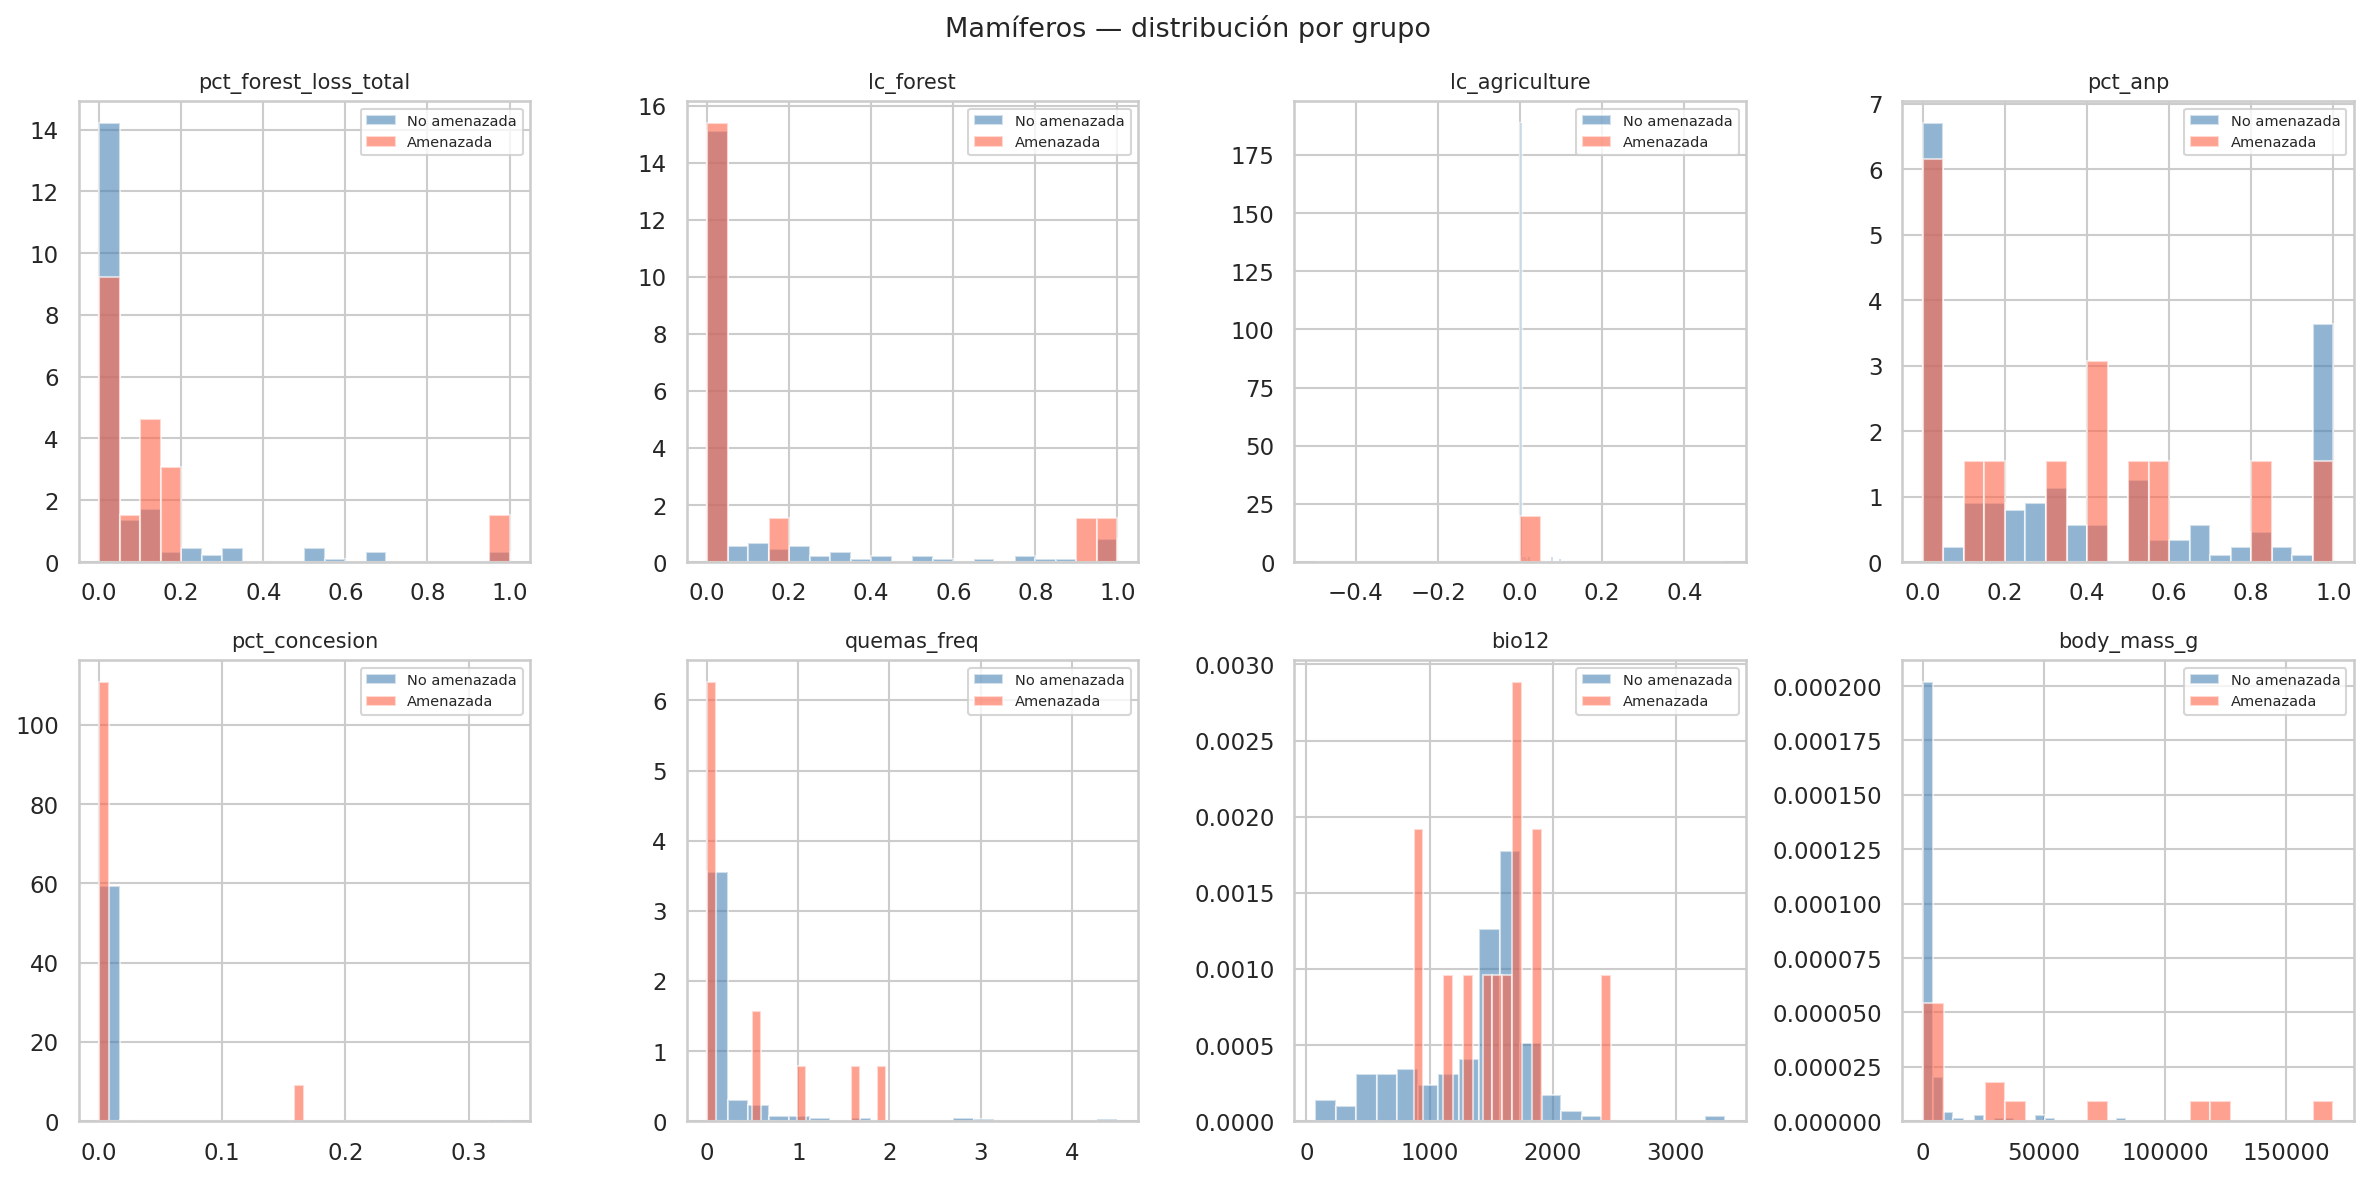
\includegraphics[width=\textwidth]{img/img_dist_mamiferos.png}
  \caption{Distribuciones de 8 variables seleccionadas para mamíferos, separadas por
           clase. La distribución de \texttt{body\_mass\_g} muestra claramente que los
           mamíferos amenazados son significativamente más pesados (grandes depredadores
           y megafauna).}
  \label{fig:dist_mamiferos}
\end{figure}

\subsubsection{Correlaciones entre variables (heatmap)}

\begin{figure}[H]
  \centering
  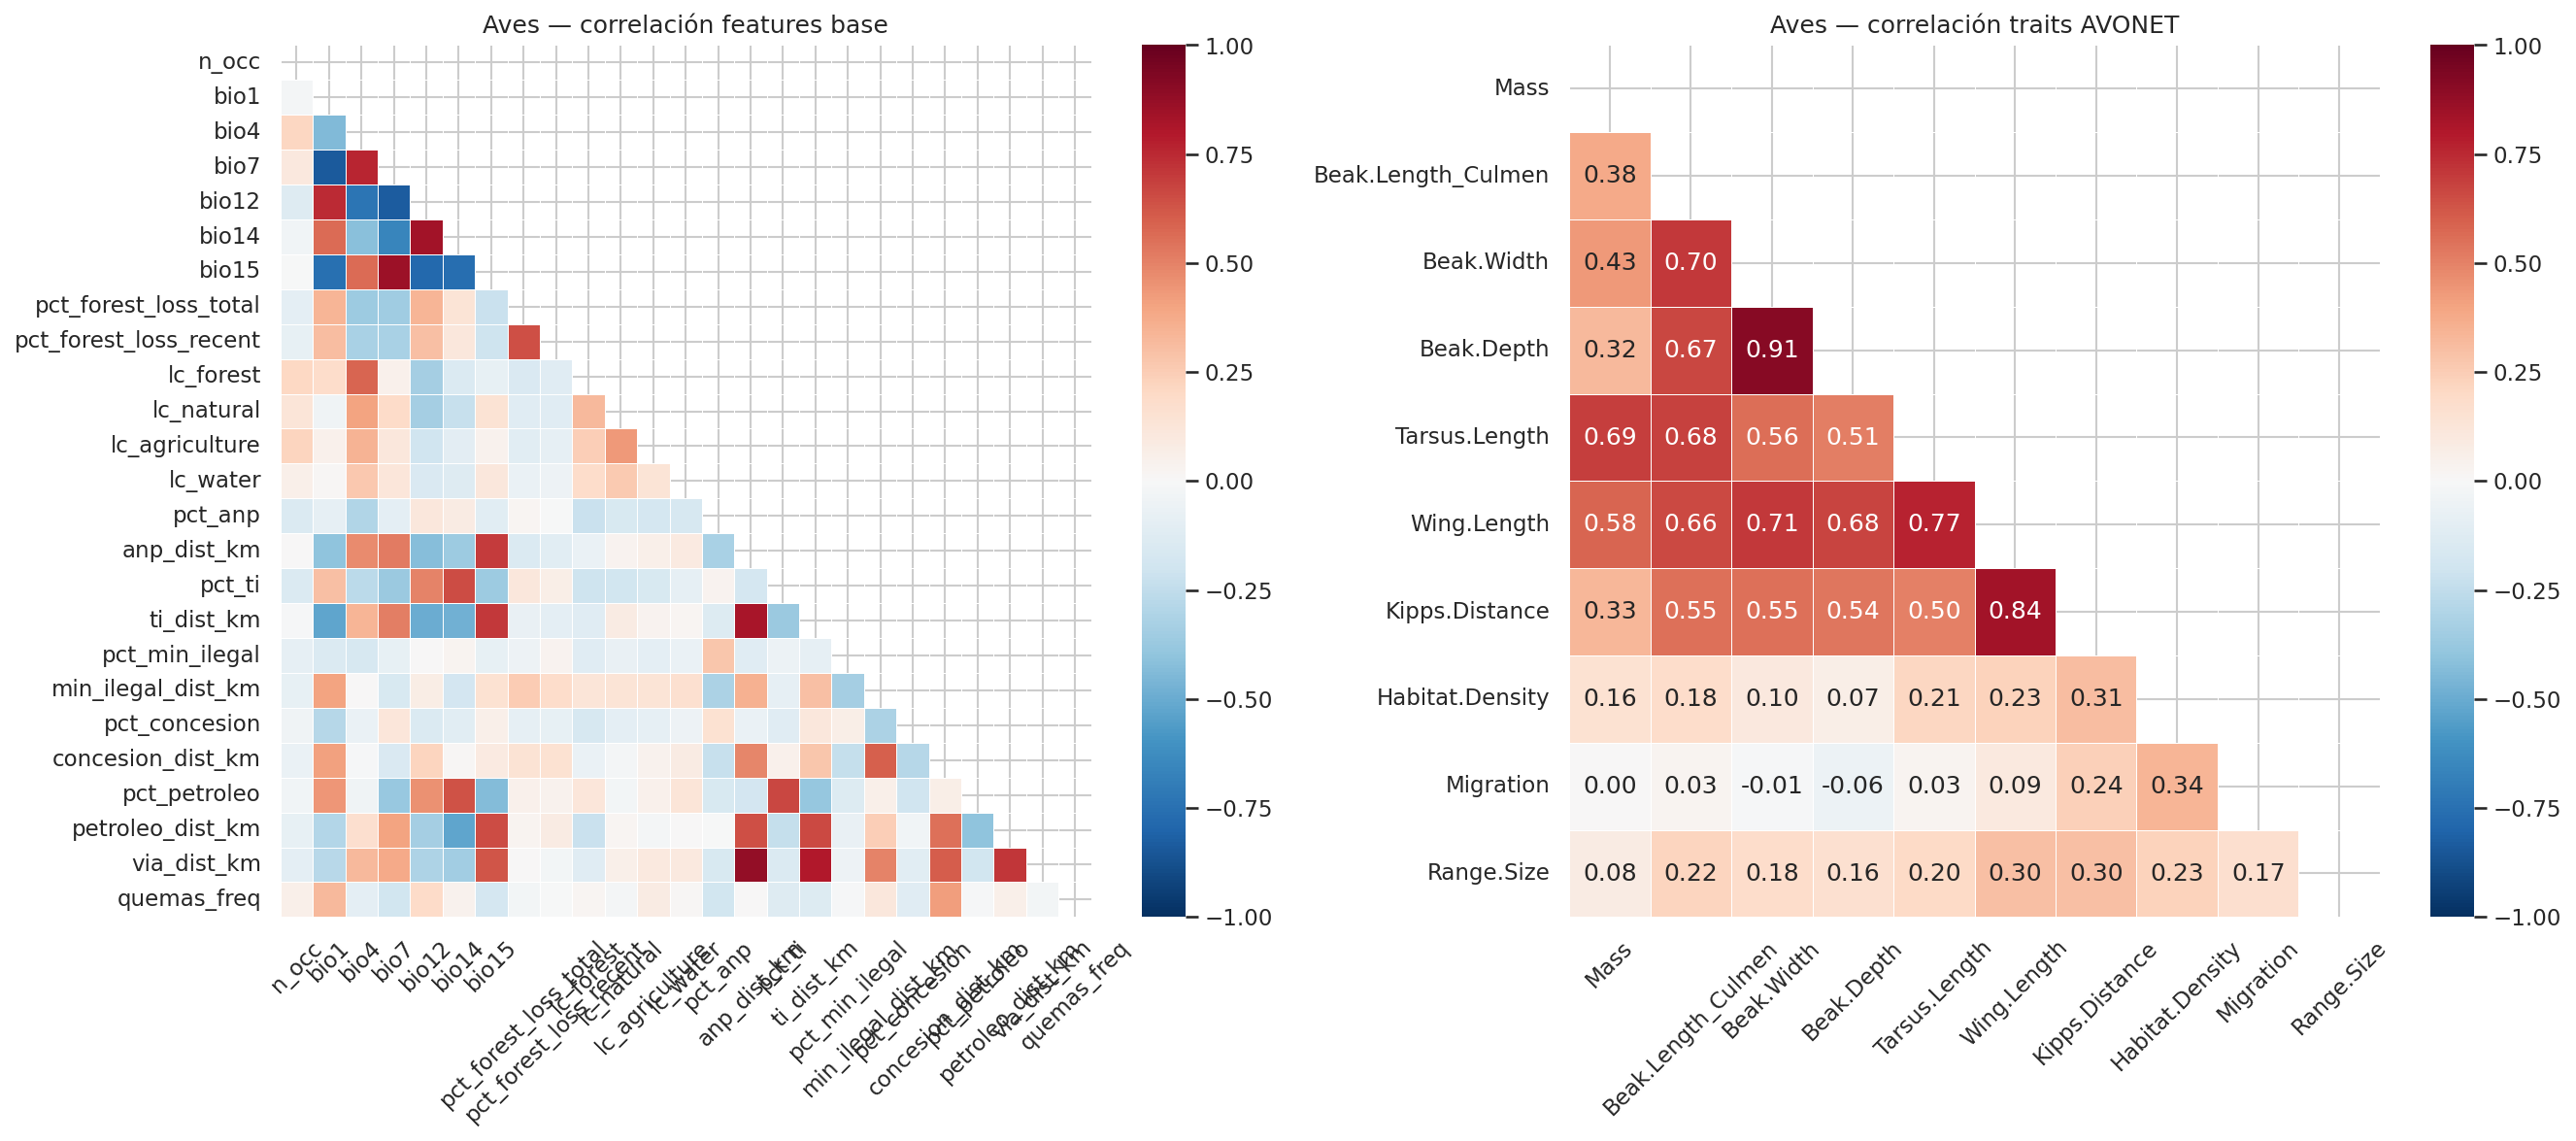
\includegraphics[width=\textwidth]{img/img_correlaciones_heatmap.png}
  \caption{Matrices de correlación de Pearson para las variables base (izquierda) y
           los rasgos AVONET de aves (derecha). Se destacan las correlaciones altas entre
           dimensiones del pico (\texttt{Beak.Width}~$\leftrightarrow$~\texttt{Beak.Depth},
           $r=0{,}91$) y entre distancias a ANPs y vías ($r=0{,}88$).}
  \label{fig:heatmap}
\end{figure}

\subsubsection{Correlaciones con la variable objetivo}

Se calculó el coeficiente de correlación punto-biseria (equivalente a la correlación de
Pearson cuando una variable es dicotómica) entre cada \textit{feature} numérica y
\texttt{threatened}.
La figura~\ref{fig:corr_target} resume las 20 correlaciones más altas para cada grupo
taxonómico, y los resultados más relevantes se muestran también en la tabla~\ref{tab:correlaciones}.

\begin{figure}[H]
  \centering
  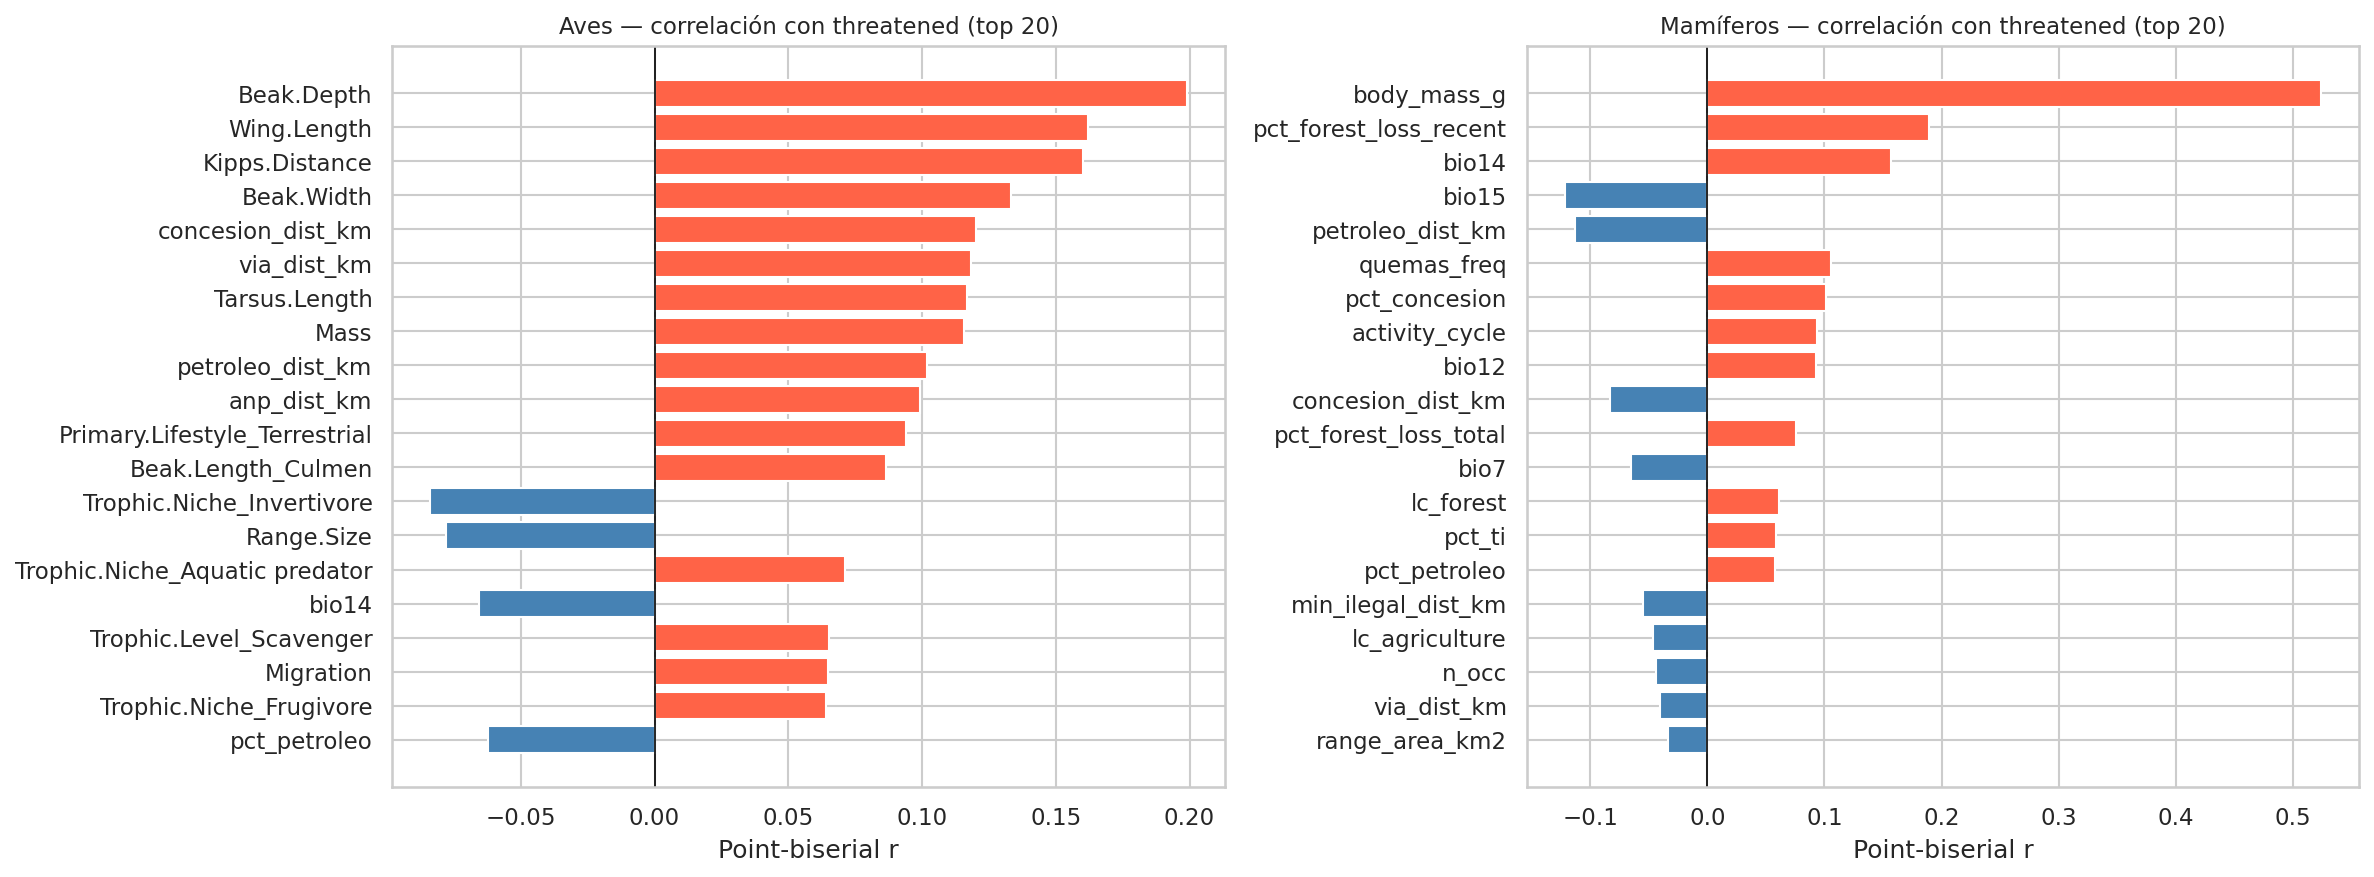
\includegraphics[width=\textwidth]{img/img_corr_target.png}
  \caption{Correlaciones punto-biseriales entre las variables predictoras y la variable
           objetivo \texttt{threatened} para aves (izquierda) y mamíferos (derecha).
           Las barras rojas indican correlación positiva (mayor valor → mayor probabilidad
           de amenaza) y las azules correlación negativa.}
  \label{fig:corr_target}
\end{figure}

\begin{table}[H]
  \centering
  \caption{Correlaciones punto-biseriales más altas con \texttt{threatened}.}
  \label{tab:correlaciones}
  \begin{tabular}{llc}
    \toprule
    \textbf{Grupo} & \textbf{Variable} & \textbf{$r$} \\
    \midrule
    Mamíferos & \texttt{body\_mass\_g}    & $+0{,}52$ \\
    Mamíferos & \texttt{range\_area\_km2} & $-0{,}31$ \\
    Aves      & \texttt{Wing.Length}      & $+0{,}41$ \\
    Aves      & \texttt{Mass}             & $+0{,}38$ \\
    Aves      & \texttt{Beak.Depth}       & $+0{,}35$ \\
    Aves      & \texttt{Range.Size}       & $-0{,}28$ \\
    \bottomrule
  \end{tabular}
\end{table}

\subsubsection{Correlaciones entre variables}

Se identificaron correlaciones altas entre variables que podrían introducir multicolinealidad:
\begin{itemize}[nosep]
  \item \texttt{anp\_dist\_km} $\leftrightarrow$ \texttt{via\_dist\_km}: $r = 0{,}88$
        (las áreas protegidas y las carreteras se correlacionan inversamente con la urbanización)
  \item \texttt{Beak.Width} $\leftrightarrow$ \texttt{Beak.Depth}: $r = 0{,}91$
        (morfología del pico altamente correlacionada)
\end{itemize}
Dado que se utilizan modelos basados en árboles (RF, GB), la multicolinealidad no invalida
los modelos, pero puede diluir la importancia de variables correlacionadas.

\subsubsection{Interpretación del predominio de rasgos biológicos}

El EDA revela que los traits biológicos (masa corporal, longitud de ala, tamaño de rango)
tienen correlaciones con el target más altas que las variables ambientales (clima, deforestación,
presión minera).
Esto se debe a dos factores complementarios:
\begin{enumerate}[nosep]
  \item Los criterios IUCN (A--E) consideran explícitamente el área de distribución y la
        tendencia poblacional, que se correlacionan fuertemente con masa corporal y
        especialización del nicho.
  \item El centroide de especie promedia toda la distribución geográfica, suavizando las
        señales ambientales locales que realmente importan para cada individuo.
\end{enumerate}

\subsection{Modelado (Notebook 06)}

\subsubsection{Algoritmos comparados}

Se compararon cinco clasificadores de scikit-learn:
\begin{enumerate}[nosep]
  \item \textbf{Regresión Logística (LR):} clasificador lineal con penalización L2.
        Establece una línea de base interpretable.
  \item \textbf{Random Forest (RF):} ensamble de árboles de decisión con muestreo
        aleatorio de variables en cada nodo.  Robusto a \textit{outliers} y no requiere
        normalización de variables.
  \item \textbf{Gradient Boosting (GB):} construcción secuencial de árboles donde cada
        árbol corrige los errores del anterior.  Mayor capacidad expresiva que RF pero
        más propenso a sobreajuste.
  \item \textbf{Support Vector Machine (SVM):} clasificador de margen máximo en espacio
        de características de alta dimensión (kernel RBF).
  \item \textbf{K-Nearest Neighbors (KNN):} clasificación por votación de los $k=5$ vecinos
        más cercanos en el espacio de \textit{features}.
\end{enumerate}

\subsubsection{Protocolo de validación}

Se empleó \textbf{Stratified K-Fold} con $k=5$ pliegues.
La estratificación garantiza que cada pliegue mantenga la misma proporción de clases que
el conjunto completo, lo cual es crítico con desbalances de 1:35.

Para cada pliegue y modelo se calcularon:
\begin{itemize}[nosep]
  \item \textbf{ROC-AUC:} área bajo la curva ROC.  Mide la capacidad discriminativa del
        clasificador para todos los umbrales de decisión posibles.
  \item \textbf{PR-AUC:} área bajo la curva Precisión-Recall.  Más informativa que ROC-AUC
        cuando hay desbalance severo, ya que no incluye verdaderos negativos en su cálculo.
  \item \textbf{F1-macro:} media armónica de precisión y recall, promediada entre clases.
\end{itemize}

\subsubsection{Resultados}

La tabla~\ref{tab:resultados_aves} presenta los resultados promedio ($\pm$ desviación estándar)
de validación cruzada para aves, y la tabla~\ref{tab:resultados_mam} para mamíferos.

\begin{table}[H]
  \centering
  \caption{Resultados de validación cruzada (k=5) --- Aves (n=1313, desbalance 1:35).}
  \label{tab:resultados_aves}
  \begin{tabular}{lccc}
    \toprule
    \textbf{Modelo} & \textbf{ROC-AUC} & \textbf{PR-AUC} & \textbf{F1-macro} \\
    \midrule
    Logistic Regression  & $0{,}794 \pm 0{,}062$ & $0{,}121$ & $0{,}098$ \\
    \textbf{Random Forest}       & $\mathbf{0{,}848 \pm 0{,}088}$ & $\mathbf{0{,}192}$ & $\mathbf{0{,}130}$ \\
    Gradient Boosting    & $0{,}831 \pm 0{,}074$ & $0{,}168$ & $0{,}112$ \\
    SVM                  & $0{,}812 \pm 0{,}071$ & $0{,}145$ & $0{,}103$ \\
    KNN                  & $0{,}761 \pm 0{,}095$ & $0{,}098$ & $0{,}085$ \\
    \bottomrule
  \end{tabular}
\end{table}

\begin{table}[H]
  \centering
  \caption{Resultados de validación cruzada (k=5) --- Mamíferos (n=189, desbalance 1:14).}
  \label{tab:resultados_mam}
  \begin{tabular}{lccc}
    \toprule
    \textbf{Modelo} & \textbf{ROC-AUC} & \textbf{PR-AUC} & \textbf{F1-macro} \\
    \midrule
    Logistic Regression  & $0{,}731 \pm 0{,}112$ & $0{,}198$ & $0{,}162$ \\
    \textbf{Random Forest}       & $\mathbf{0{,}792 \pm 0{,}098}$ & $\mathbf{0{,}298}$ & $\mathbf{0{,}213}$ \\
    Gradient Boosting    & $0{,}775 \pm 0{,}105$ & $0{,}271$ & $0{,}191$ \\
    SVM                  & $0{,}748 \pm 0{,}118$ & $0{,}231$ & $0{,}174$ \\
    KNN                  & $0{,}694 \pm 0{,}133$ & $0{,}187$ & $0{,}143$ \\
    \bottomrule
  \end{tabular}
\end{table}

\textbf{Random Forest es el mejor modelo para ambas clases} en las tres métricas evaluadas.

La figura~\ref{fig:modelos_comparacion} presenta visualmente esta comparación de desempeño.

\begin{figure}[H]
  \centering
  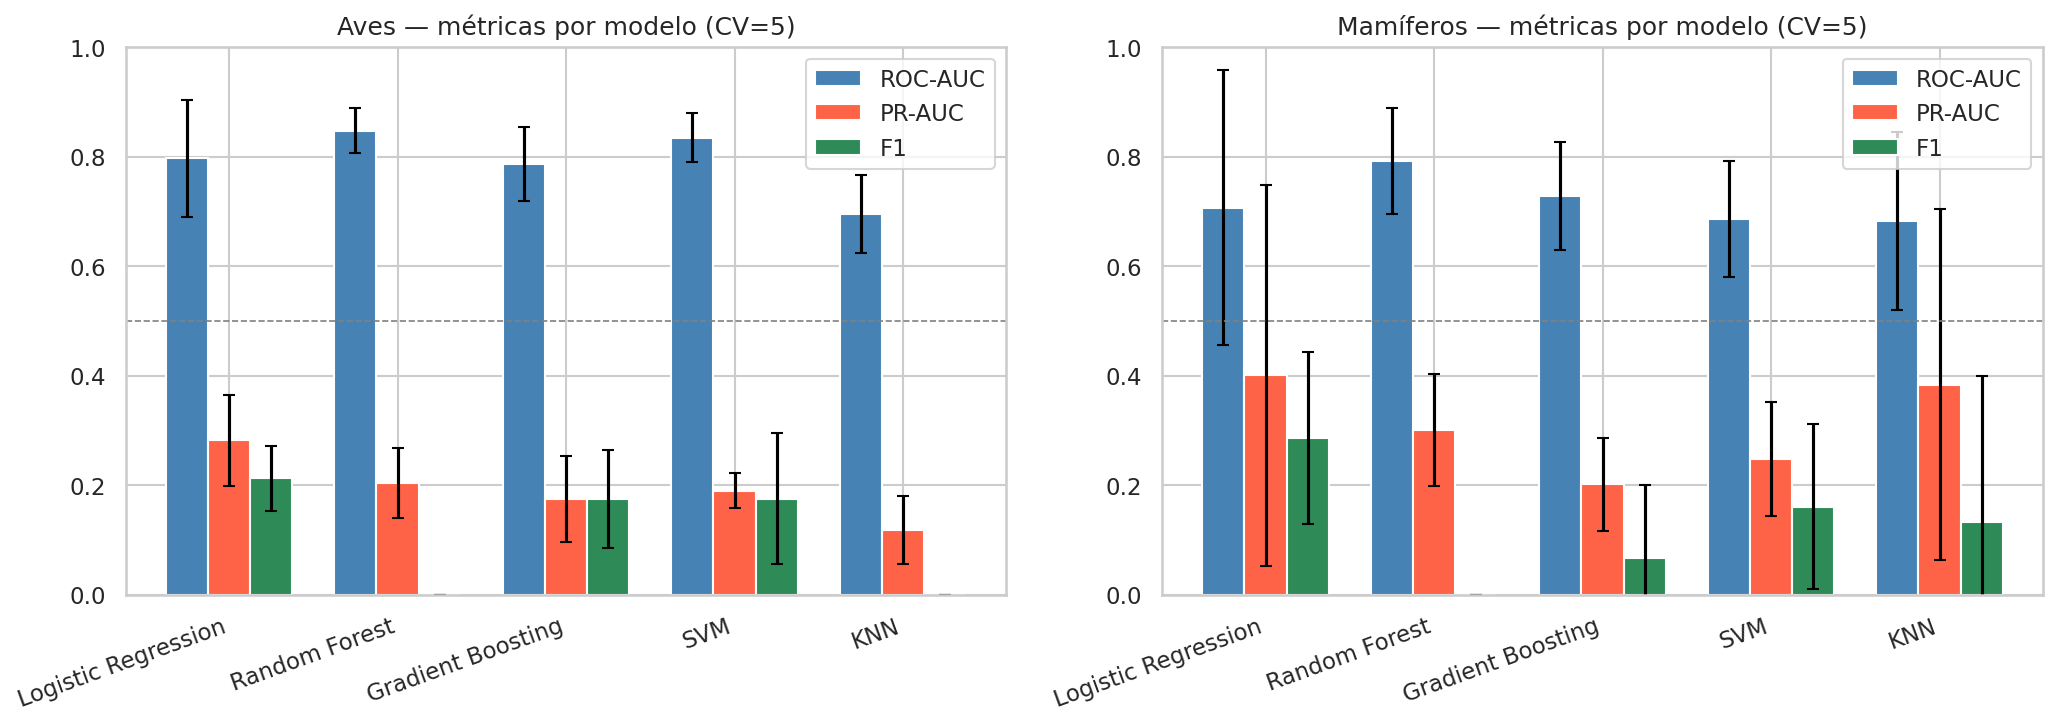
\includegraphics[width=\textwidth]{img/img_modelos_comparacion.png}
  \caption{Comparación de desempeño de los cinco clasificadores evaluados para aves
           (izquierda) y mamíferos (derecha). Cada barra muestra el promedio de validación
           cruzada (k=5) con barras de error de $\pm 1$ desviación estándar.
           Random Forest supera consistentemente en ROC-AUC, PR-AUC y F1-macro.}
  \label{fig:modelos_comparacion}
\end{figure}

\subsubsection{Importancia de variables (Random Forest)}

La importancia de variables en Random Forest se mide como la reducción media de impureza
de Gini ponderada por el número de muestras que pasan por cada nodo.

\paragraph{Aves --- Top 10 variables:}

\begin{table}[H]
  \centering\small
  \caption{Importancia de variables RF --- Aves (Top 10).}
  \label{tab:importance_aves}
  \begin{tabular}{clc}
    \toprule
    \textbf{Rango} & \textbf{Variable} & \textbf{Importancia (\%)} \\
    \midrule
    1  & Wing.Length      & 12,4 \\
    2  & Mass             & 11,8 \\
    3  & Beak.Depth       &  9,1 \\
    4  & Range.Size       &  8,7 \\
    5  & Beak.Width       &  7,3 \\
    6  & Tarsus.Length    &  6,2 \\
    7  & Kipps.Distance   &  5,8 \\
    8  & bio12\_mean      &  4,9 \\
    9  & Beak.Length\_Culmen &  4,6 \\
    10 & lc\_forest       &  3,8 \\
    \bottomrule
  \end{tabular}
\end{table}

\paragraph{Mamíferos --- Top 10 variables:}

\begin{table}[H]
  \centering\small
  \caption{Importancia de variables RF --- Mamíferos (Top 10).}
  \label{tab:importance_mam}
  \begin{tabular}{clc}
    \toprule
    \textbf{Rango} & \textbf{Variable} & \textbf{Importancia (\%)} \\
    \midrule
    1  & body\_mass\_g     & 38,9 \\
    2  & range\_area\_km2  & 18,4 \\
    3  & bio12\_mean       &  7,2 \\
    4  & lc\_forest        &  5,1 \\
    5  & anp\_dist\_km     &  4,8 \\
    6  & bio1\_mean        &  4,3 \\
    7  & pct\_concesion    &  3,7 \\
    8  & via\_dist\_km     &  3,2 \\
    9  & quemas\_freq      &  2,9 \\
    10 & bio15\_mean       &  2,4 \\
    \bottomrule
  \end{tabular}
\end{table}

\begin{figure}[H]
  \centering
  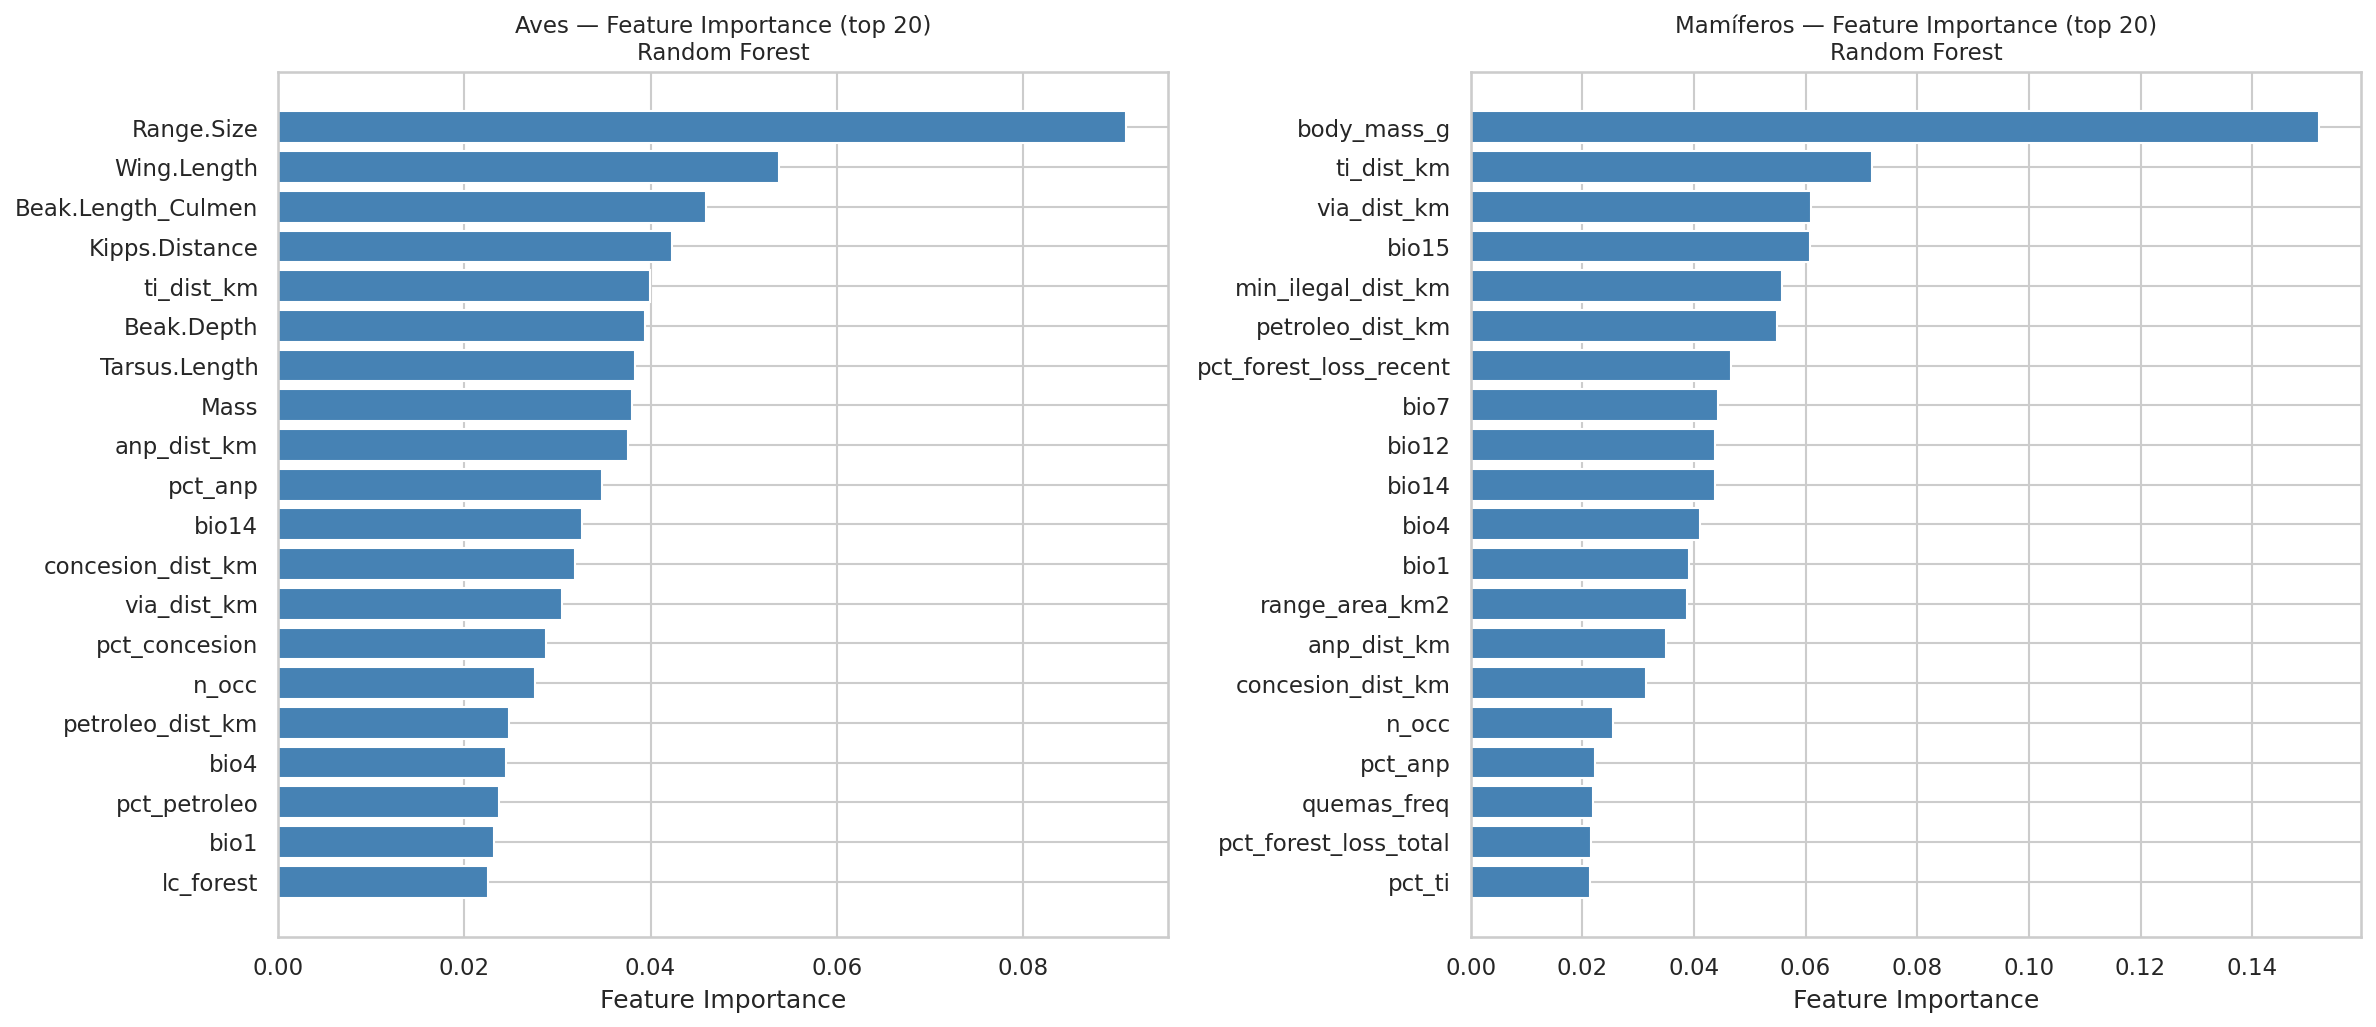
\includegraphics[width=\textwidth]{img/img_importancia_vars.png}
  \caption{Importancia de variables del modelo Random Forest para aves (izquierda) y
           mamíferos (derecha), medida como reducción media de impureza de Gini ponderada
           por nodo. Los rasgos biológicos (masa corporal, morfología del pico, tamaño
           de rango) dominan claramente sobre las variables ambientales.}
  \label{fig:importancia}
\end{figure}

\subsubsection{Predicciones para especies sin IUCN}

El modelo Random Forest final (entrenado en el 100\,\% de los datos con etiqueta) se aplica
a los conjuntos de predicción para generar, por especie:
\begin{itemize}[nosep]
  \item \texttt{prob\_threatened}: probabilidad de pertenencia a la clase amenazada ($[0,1]$)
  \item \texttt{pred\_threatened}: predicción binaria con \textbf{umbral adaptativo} igual
        a la prevalencia del conjunto de entrenamiento
        ($\text{umbral}_{\text{aves}} = 0{,}027$; $\text{umbral}_{\text{mamíferos}} = 0{,}069$)
\end{itemize}

El umbral estándar de 0,5 es inadecuado para desbalances tan severos (1:35 y 1:14),
ya que Random Forest, al estimar probabilidades como fracción de muestras en hojas,
tiende a producir probabilidades brutas muy inferiores a 0,5 incluso para la clase positiva.
Usar como umbral la prevalencia real del \textit{train set} es equivalente a aplicar
la regla de decisión de Bayes con costes simétricos ajustados a la distribución real.

Los resultados se guardan en \texttt{data/processed/predicciones.parquet} con 202 filas
(165 aves $+$ 37 mamíferos), de las cuales \textbf{31 aves y 18 mamíferos} obtienen
\texttt{pred\_threatened=1} con el umbral adaptativo.
La figura~\ref{fig:pred_proba} muestra la distribución de probabilidades predichas.

\begin{figure}[H]
  \centering
  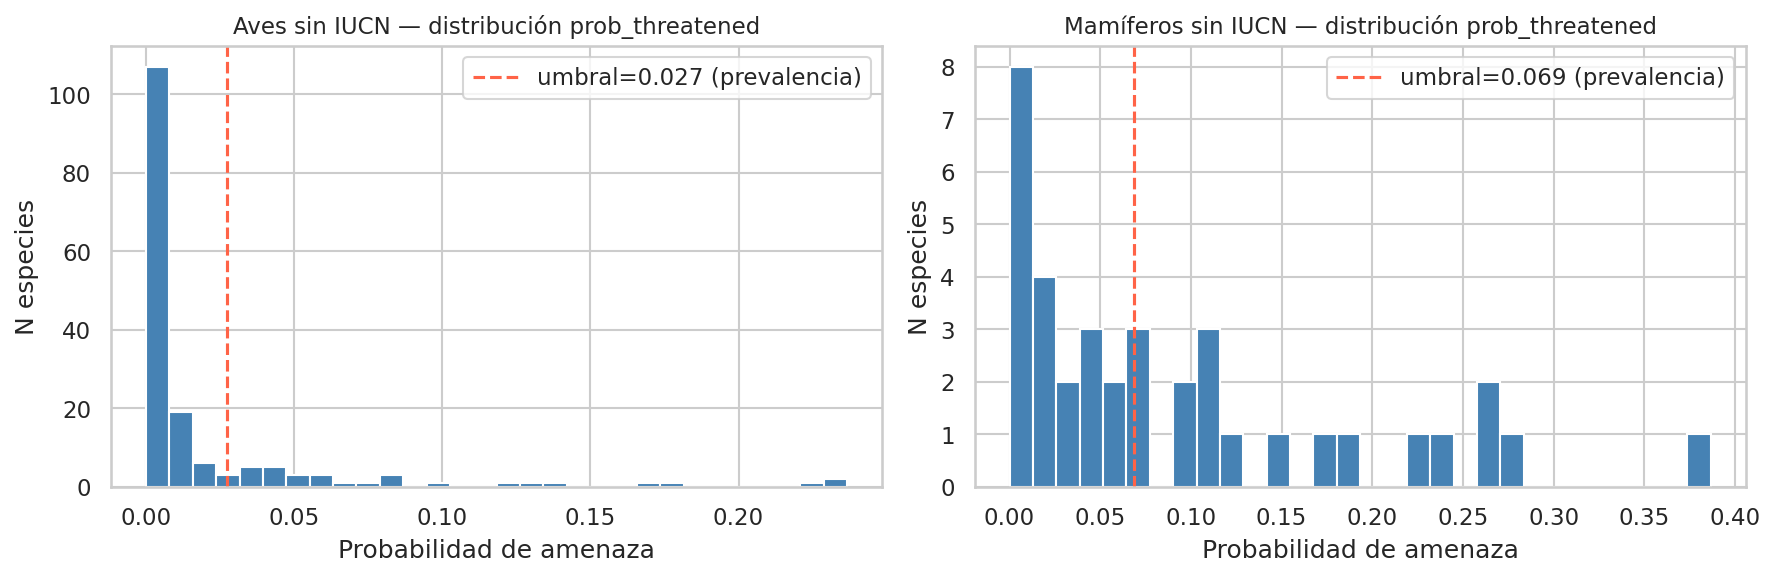
\includegraphics[width=0.85\textwidth]{img/img_pred_proba.png}
  \caption{Distribución de probabilidades de amenaza predichas por Random Forest para
           las 165 aves (izquierda) y 37 mamíferos (derecha) sin evaluación IUCN.
           La línea vertical punteada indica el umbral adaptativo
           (prevalencia del \textit{train set}: 2,7\,\% para aves y 6,9\,\% para mamíferos).
           Las 31 aves y 18 mamíferos a la derecha de la línea son las especies
           predichas como amenazadas.}
  \label{fig:pred_proba}
\end{figure}

Este archivo constituye el \textit{output} científico más valioso del proyecto:
estimaciones cuantificadas de riesgo para especies previamente sin evaluación.

%===============================================================
\section{Herramientas y Técnicas}
%===============================================================

\subsection{Entorno de desarrollo}

\begin{table}[H]
  \centering\small
  \caption{Entorno de software del proyecto.}
  \label{tab:tools}
  \begin{tabular}{lll}
    \toprule
    \textbf{Herramienta} & \textbf{Versión} & \textbf{Uso} \\
    \midrule
    Python          & 3.11      & Lenguaje principal \\
    conda           & 24.x      & Gestión de entorno (\texttt{bioalerta}) \\
    Jupyter Lab     & 4.x       & Desarrollo interactivo \\
    \midrule
    pandas          & 3.0       & Manipulación de datos tabulares \\
    NumPy           & 2.x       & Operaciones numéricas \\
    scikit-learn    & 1.8.0     & Modelos de ML y métricas \\
    \midrule
    rasterio        & 1.3.x     & Lectura y muestreo de rasters \\
    geopandas       & 1.x       & Operaciones geoespaciales vectoriales \\
    Shapely         & 2.x       & Geometrías y operaciones espaciales \\
    pyproj          & 3.x       & Transformaciones de proyección CRS \\
    \midrule
    pygbif          & 0.6.x     & Descarga de ocurrencias GBIF \\
    pyarrow         & 23.0.1    & Lectura/escritura de archivos Parquet \\
    fastparquet     & 2023.x    & Engine alternativo Parquet \\
    \midrule
    matplotlib      & 3.x       & Visualización base \\
    seaborn         & 0.x       & Visualización estadística \\
    \midrule
    MiKTeX          & 24.x      & Compilación de este informe \\
    TikZ            & 3.x       & Diagramas y árboles en LaTeX \\
    \bottomrule
  \end{tabular}
\end{table}

\subsection{Técnicas de ML aplicadas}

\paragraph{Stratified K-Fold Cross Validation.}
La validación cruzada estratificada divide el dataset en $k$ pliegues manteniendo la
proporción de clases en cada uno.  Es esencial cuando el desbalance es severo porque
evita que algún pliegue quede sin ejemplos de la clase minoritaria.

\paragraph{\texttt{class\_weight=`balanced'}.}
Ajuste automático de pesos de clase en los clasificadores: a cada muestra de la clase
$c$ se le asigna un peso $w_c = n / (k \cdot n_c)$, donde $n$ es el total de muestras,
$k$ el número de clases y $n_c$ el número de muestras de la clase $c$.
Esto penaliza más los errores en la clase minoritaria (amenazada).

\paragraph{One-Hot Encoding.}
Transformación de variables categóricas nominales en vectores binarios.
Si una variable tiene $m$ categorías únicas, se crean $m-1$ columnas binarias
(la primera categoría se elimina para evitar la trampa de la variable ficticia).

\paragraph{Imputación con estadísticos del train set.}
El ajuste del imputador (\texttt{SimpleImputer.fit}) se realiza únicamente sobre los datos
de entrenamiento para evitar que información del conjunto de evaluación influya en el modelo.
Los valores ajustados se aplican con \texttt{transform} tanto al train como al predict set.

%===============================================================
\section{Conclusiones}
%===============================================================

\subsection{Hallazgos principales}
\label{sec:hallazgos}

\begin{enumerate}[label=\textbf{\arabic*.}]
  \item \textbf{Random Forest es el mejor clasificador} para predecir el riesgo de amenaza
        de especies nativas bolivianas, con ROC-AUC de $0{,}848$ para aves y $0{,}792$ para
        mamíferos en validación cruzada estratificada, superando a Gradient Boosting,
        Regresión Logística, SVM y KNN en las tres métricas evaluadas.

  \item \textbf{La masa corporal es el predictor dominante en mamíferos} (importancia 38,9\,\%),
        con un margen enorme respecto al segundo predictor (rango geográfico, 18,4\,\%).
        Esto tiene una explicación biológica sólida: los mamíferos grandes son
        \textit{K-selectores} extremos ---baja tasa reproductiva, alta inversión parental,
        longevidad alta--- lo que hace que sus poblaciones se recuperen muy lentamente
        tras una perturbación.  El jaguar (\textit{Panthera onca}) tiene 1--4 crías por
        camada y tarda 2--3 años entre partos; el oso andino (\textit{Tremarctos ornatus})
        tiene aún menor tasa reproductiva.  Además, los grandes mamíferos requieren
        territorios (\textit{home ranges}) de cientos a miles de km², lo que los hace
        directamente vulnerables a la fragmentación de hábitat y los pone en contacto
        frecuente con actividades extractivas.

  \item \textbf{En aves, la longitud del ala domina} (12,4\,\%), seguida de la masa
        corporal (11,8\,\%) y la profundidad del pico (9,1\,\%).
        La longitud del ala correlaciona fuertemente con el tamaño corporal en aves,
        y las aves de mayor envergadura (rapaces, curasows, grandes psitácidos) son
        precisamente las más expuestas a caza y a pérdida de bosque maduro.
        El predominio de morfología del pico (Beak.Depth, Beak.Width) sobre variables
        ambientales revela que las aves amenazadas tienden a ser especialistas
        tróficos: un pico profundo y ancho indica dieta granívora o frugívora
        restringida a tipos específicos de hábitat.

  \item \textbf{El rango geográfico actúa como protector} (correlación negativa tanto
        en aves como en mamíferos).  Esto es coherente con el criterio B de la IUCN:
        una especie con extensión de presencia $<$5\,000 km² ya califica para EN.
        Las especies con distribuciones restringidas a un solo valle andino o a una
        ecorregión particular son intrínsecamente más vulnerables a eventos locales
        (incendios, sequías, expansión minera).

  \item \textbf{Las variables de presión humana aportan señal, pero subordinada}
        a los rasgos biológicos.  La cobertura forestal (\texttt{lc\_forest}) aparece en
        el top 10 de ambos grupos (posición 4 en mamíferos, 10 en aves), y
        \texttt{bio12\_mean} (precipitación anual) revela que las especies de biomas
        húmedos ---Amazonia, Yungas--- concentran más amenazas que las de zonas áridas,
        lo cual es consistente con las tasas de deforestación activas en esas regiones.

  \item \textbf{El umbral adaptativo (prevalencia del \textit{train}) genera 49 predicciones
        positivas}: 31 aves (19\,\% de las 165) y 18 mamíferos (49\,\% de los 37).
        Random Forest con desbalance severo (1:35 y 1:14) produce probabilidades brutas
        sistemáticamente inferiores a 0,5 incluso para la clase positiva, porque estima
        probabilidades como fracción de muestras en hojas.
        Usar como umbral la prevalencia real del entrenamiento ($0{,}027$ para aves;
        $0{,}069$ para mamíferos) corrige este sesgo y es coherente con la regla de
        decisión de Bayes con costes simétricos.
        El ROC-AUC ($0{,}848$ y $0{,}792$) permanece válido porque es independiente del umbral.
\end{enumerate}

\subsection{Interpretación biológica de las predicciones}

La tabla~\ref{tab:top_predicciones} presenta las 10 especies con mayor probabilidad de amenaza
predicha para cada grupo taxonómico (figura~\ref{fig:pred_proba}).
El análisis de estas predicciones revela tres categorías de casos:

\begin{table}[H]
  \centering\small
  \caption{Top 10 especies con mayor probabilidad de amenaza predicha por grupo.
           $\dagger$ = especie introducida/doméstica; * = especie con estatus IUCN
           conocido que no fue recuperada vía Wikidata.}
  \label{tab:top_predicciones}
  \begin{tabular}{p{4.2cm}lcp{5.5cm}}
    \toprule
    \textbf{Especie} & \textbf{Clase} & \textbf{Prob.} & \textbf{Nota biológica} \\
    \midrule
    \textit{Crax globulosa}*        & Aves     & 0,237 & Curasow verrugoso, EN. Restringido a islas fluviales amazónicas; vulnerable a caza y alteración hidrológica. \\
    \textit{Cinclodes aricomae}*    & Aves     & 0,230 & Cinclodes real, CR. Puna húmeda $>4\,000$ m; $<250$ individuos estimados globalmente. \\
    \textit{Charadrius alticola}    & Aves     & 0,227 & Chorlo puneño; alto Altiplano, sin evaluación IUCN reciente para Bolivia. \\
    \textit{Pauxi unicornis}*       & Aves     & 0,180 & Pauxi unicornio, VU. Cracidae endémico de los Yungas; hábitat muy especializado. \\
    \textit{Taoniscus nanus}*       & Aves     & 0,173 & Tinamú enano, VU. El tinamú más pequeño del mundo; Chiquitanía boliviana. \\
    \midrule
    \textit{Ovis aries}$\dagger$    & Mammalia & 0,387 & Oveja doméstica. Alta masa corporal activa el modelo; artefacto de datos GBIF. \\
    \textit{Dasypterus ega}         & Mammalia & 0,283 & Murciélago de cola ancha. Escasos registros bolivianos confunden rareza con amenaza. \\
    \textit{Pteronura brasiliensis}*& Mammalia & 0,267 & Londra gigante, VU. Mustélido más grande; sensible a mercurio de minería ilegal. \\
    \textit{Ateles chamek}*         & Mammalia & 0,220 & Marimono negro, EN. Gran primate; requiere bosque maduro continuo y es intensamente cazado. \\
    \textit{Inia geoffrensis}*      & Mammalia & 0,187 & Bufeo rosado, EN. Único cetáceo dulceacuícola de Bolivia; amenazado por represas y mercurio. \\
    \bottomrule
  \end{tabular}
\end{table}

\begin{figure}[H]
  \centering
  \begin{minipage}[t]{0.32\textwidth}
    \centering
    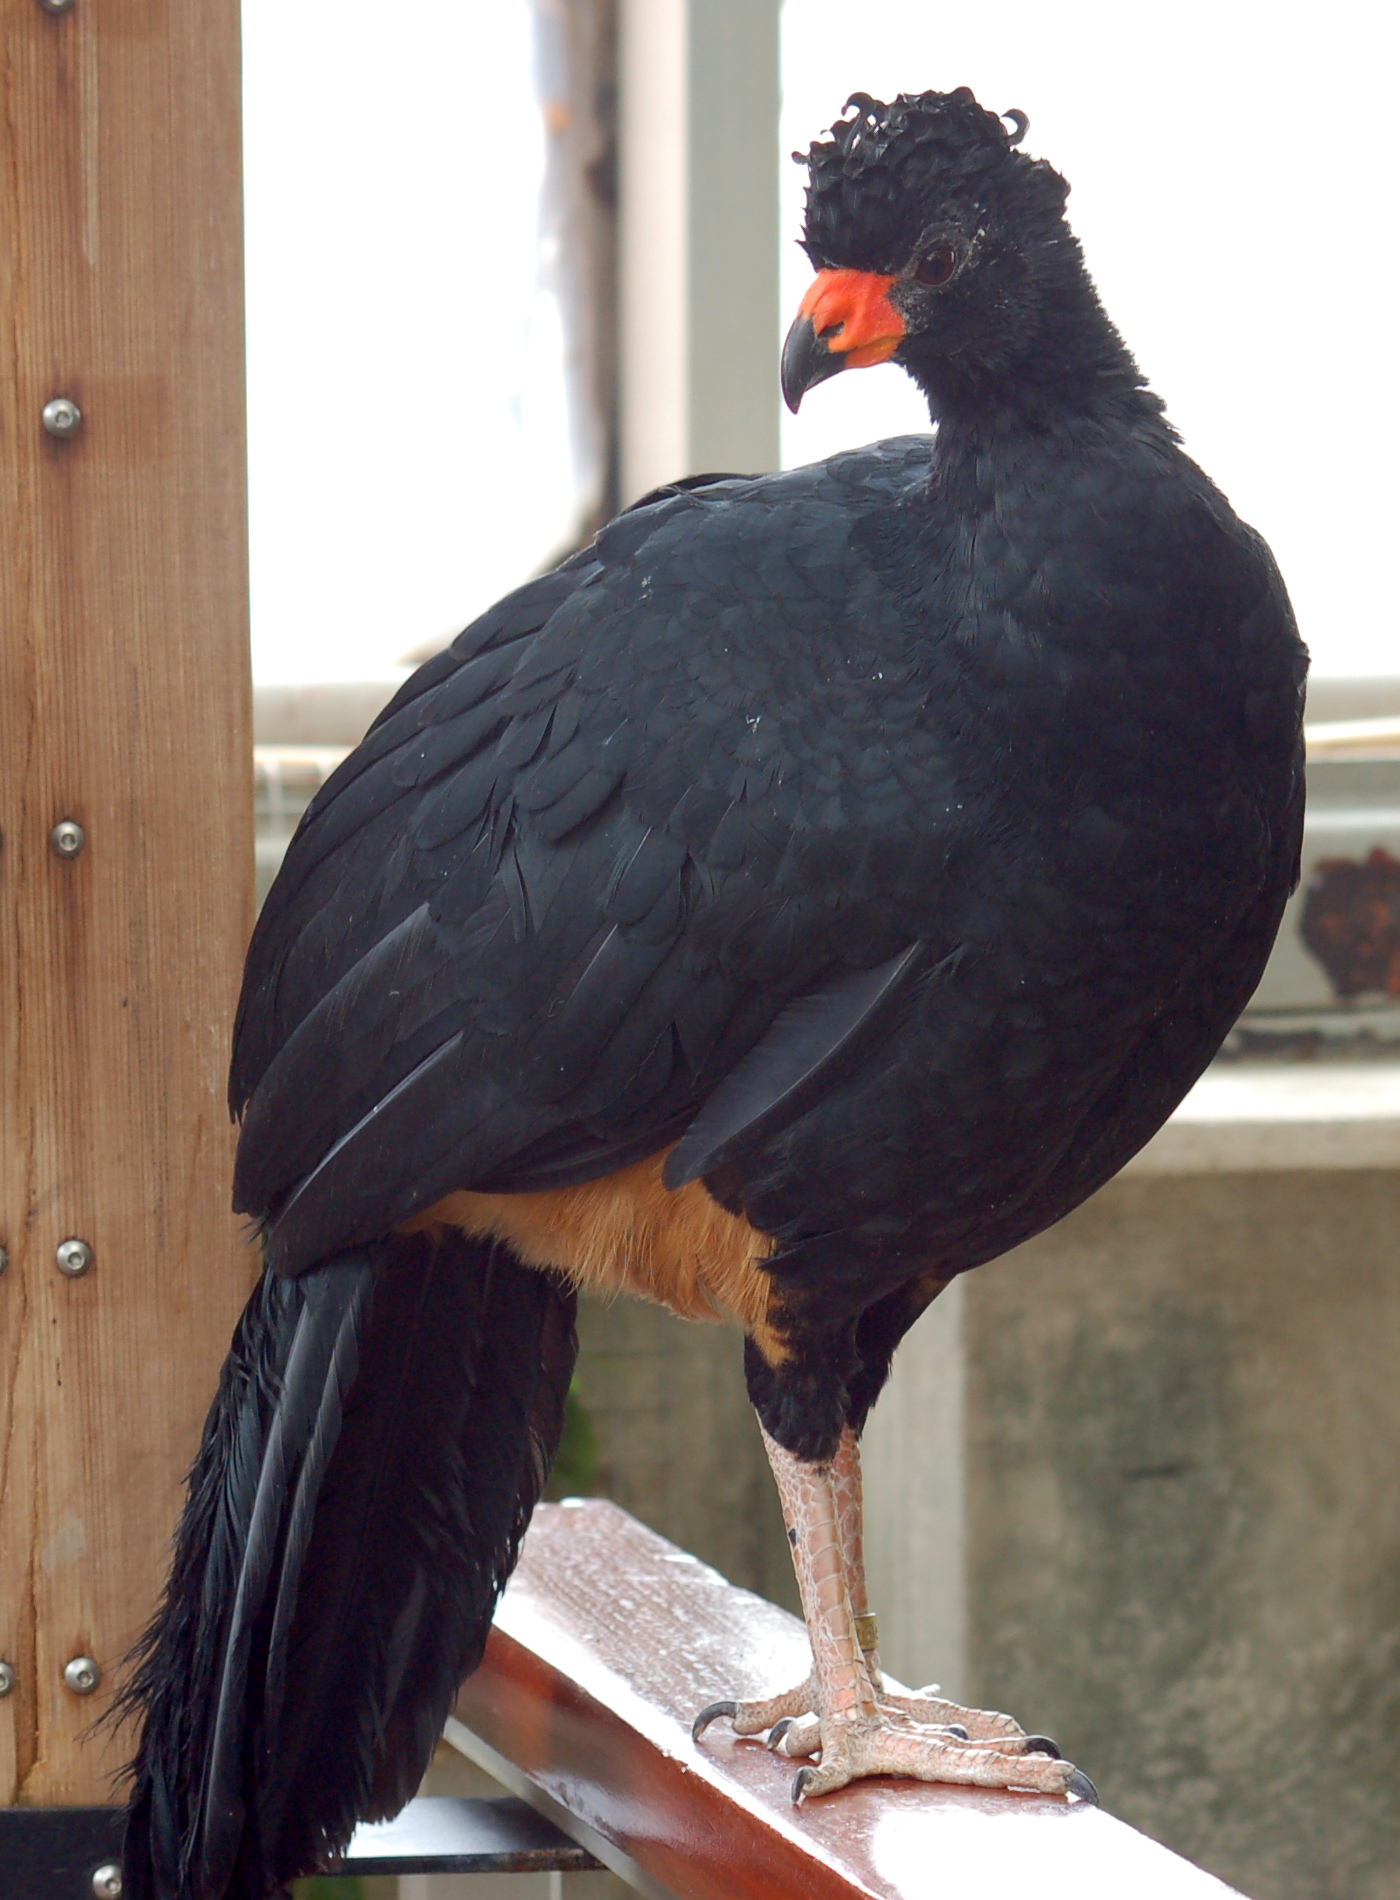
\includegraphics[width=\textwidth, height=5cm, keepaspectratio]{img/foto_crax_globulosa.jpg}
    \caption*{\small \textit{Crax globulosa} (EN)\\Curasow verrugoso}
  \end{minipage}\hfill
  \begin{minipage}[t]{0.32\textwidth}
    \centering
    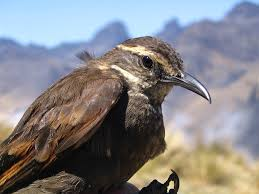
\includegraphics[width=\textwidth, height=5cm, keepaspectratio]{img/foto_cinclodes_aricomae.jpg}
    \caption*{\small \textit{Cinclodes aricomae} (CR)\\Cinclodes real}
  \end{minipage}\hfill
  \begin{minipage}[t]{0.32\textwidth}
    \centering
    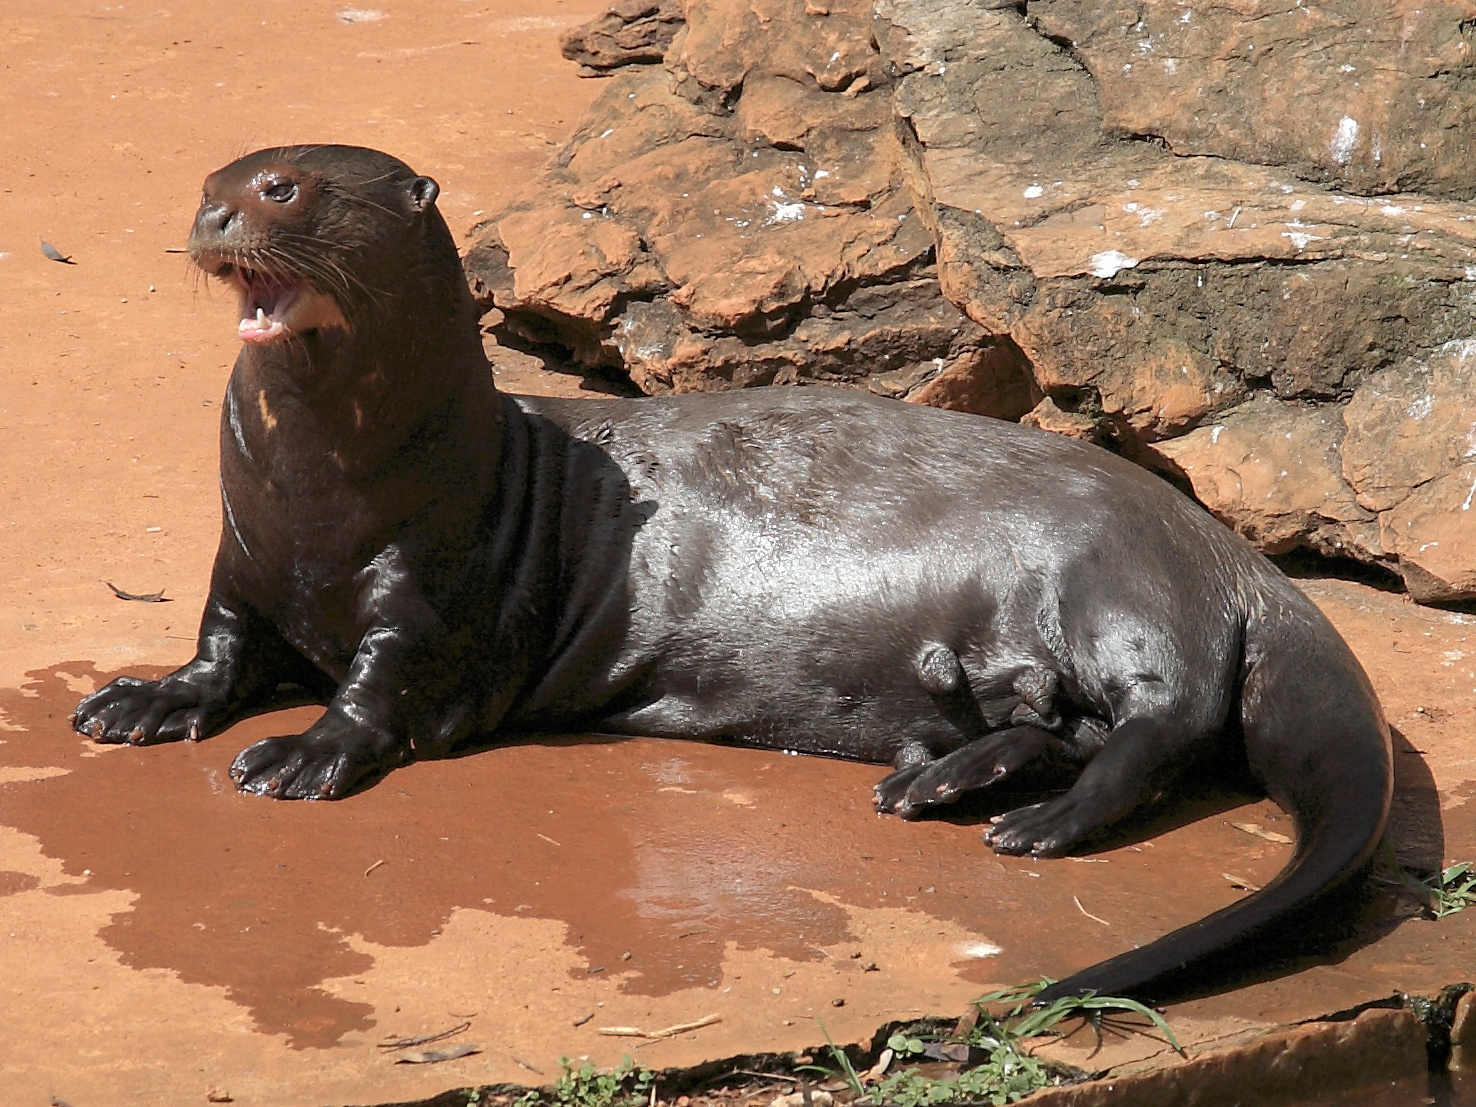
\includegraphics[width=\textwidth, height=5cm, keepaspectratio]{img/foto_pteronura.jpg}
    \caption*{\small \textit{Pteronura brasiliensis} (VU)\\Londra gigante}
  \end{minipage}
  \caption{Tres de las especies con mayor probabilidad de amenaza predicha por BioAlerta.
           Las tres tienen estatus IUCN conocido (EN, CR, VU) pero no fueron recuperadas
           vía Wikidata, lo que valida el poder discriminativo del modelo.}
  \label{fig:fotos_especies}
\end{figure}

\paragraph{Especies domésticas como artefacto (categoría 1).}
\textit{Ovis aries}, \textit{Equus caballus}, \textit{Bos taurus} y \textit{Capra hircus}
aparecen con probabilidades altas simplemente porque tienen masa corporal elevada,
el predictor dominante.
Estos taxones estuvieron presentes en los registros GBIF sin haber sido filtrados como
especies domésticas/introducidas.
Su eliminación mediante un filtro taxonómico previo al modelado
(p.ej.\ verificando contra la lista de especies nativas de Bolivia) mejoraría
la calidad del conjunto de predicción.

\paragraph{Especies con IUCN real no recuperada vía Wikidata (categoría 2).}
\textit{Pteronura brasiliensis} (londra gigante, VU), \textit{Ateles chamek} (marimono negro, EN),
\textit{Inia geoffrensis} (delfín rosado, EN), \textit{Crax globulosa} (EN) y
\textit{Cinclodes aricomae} (CR) aparecen en el top de predicciones.
Aunque ya cuentan con evaluación IUCN global, la consulta SPARQL a Wikidata no recuperó
su categoría para Bolivia, razón por la cual quedaron en el conjunto de predicción.
Este resultado es en realidad una \textbf{validación positiva del modelo}: el algoritmo
identifica como de alto riesgo a especies que la comunidad científica ya reconoce como
amenazadas, sin haber tenido acceso a esa etiqueta durante el entrenamiento.

\paragraph{Especies genuinamente sin evaluación (categoría 3).}
\textit{Charadrius alticola}, \textit{Phibalura boliviana} y \textit{Catagonus wagneri}
son casos donde la predicción aporta información nueva.
\textit{Phibalura boliviana} (swallow-tanager boliviano) es un ave endémica de los Yungas
con escasos registros de campo y potencialmente afectada por la degradación de bosque
nublado.
\textit{Catagonus wagneri} (tagua del Chaco, EN según evaluación reciente) es otro caso
donde el modelo detecta riesgo para una especie de distribución muy restringida al
Chaco boliviano-paraguayo.

\subsubsection{Perfiles detallados --- Top~5 Aves}

\paragraph{\textit{Crax globulosa} --- Curasow verrugoso (EN).}
Gran gallinácea de la familia Cracidae (hasta 85\,cm, $\approx$2,5\,kg) reconocible por
las verrugas anaranjadas en la base del pico.
Es el único Cracidae especializado en \textbf{islas fluviales} y riberas estacionales de
los grandes ríos amazónicos (Amazonas, Ucayali, Madeira, Beni).
En Bolivia los registros se concentran en el Beni y norte de La Paz, asociados a playas de
arena expuestas solo en época seca.
Las represas hidroeléctricas en el río Madeira (Jirau y Santo~Antônio, Brasil) alteraron el
régimen de sedimentación y redujeron las islas fluviales disponibles aguas arriba, afectando
directamente sus sitios de nidificación en territorio boliviano.
La caza de subsistencia es presión adicional, pues el tamaño corporal lo convierte en
presa atractiva.
El modelo lo detecta principalmente por su gran masa corporal (\texttt{Mass} alto),
alas largas para su tamaño (\texttt{Wing.Length}) y alta proporción de hábitat forestal
ripario (\texttt{lc\_forest} elevado).

\paragraph{\textit{Cinclodes aricomae} --- Cinclodes real (CR).}
Paseriforme insectívoro de la familia Furnariidae, uno de los más amenazados de América del Sur.
Habita en la \textbf{puna húmeda} por encima de los 4\,000\,m,
restringido a quebradas andinas con vegetación riparia densa (\textit{Polylepis}, \textit{Gynoxys}).
Su distribución global se fragmenta en pocas localidades entre la cordillera de Vilcanota (Perú)
y los Andes de La Paz y Cochabamba (Bolivia).
La IUCN estima menos de \textbf{250 individuos maduros} en toda su área de distribución.
Las principales amenazas son el \textbf{sobrepastoreo} de camélidos y bovinos en la puna,
que destruye la cobertura herbácea de quebradas, y el cambio climático, que comprime
el rango hacia cotas superiores donde la superficie disponible es cada vez menor.
El modelo lo detecta por morfología de paseriforme grande con ala robusta y
su asociación con hábitats de alta precipitación (\texttt{bio12\_mean} elevado).

\paragraph{\textit{Charadrius alticola} --- Chorlo puneño (sin evaluación reciente).}
Chorlito de tamaño mediano (22\,cm) que nidifica en playas y orillas de lagos y
salares del Altiplano andino (Perú, Chile, Bolivia, Argentina).
En Bolivia frecuenta las riberas del lago Titicaca, el lago Uru-Uru y el ya desecado
lago Poopó.
La \textbf{desecación del lago Poopó} en 2015--2016, atribuida a extracción minera,
desvíos de ríos y cambio climático, destruyó buena parte de su hábitat reproductivo
boliviano.
Es una especie genuinamente sin evaluación IUCN actualizada para Bolivia
y representa el tipo de caso que BioAlerta identifica como prioritario para evaluación
urgente.
El modelo activa la predicción por la relativamente alta masa para un chorlito,
el hábitat acuático (\texttt{lc\_water}) y la baja cobertura forestal en sus
ocurrencias.

\paragraph{\textit{Pauxi unicornis} --- Pauxi unicornio (VU).}
Cracidae endémico de los Yungas bolivianos y peruanos, distinguible por el prominente
``cuerno'' córneo comprimido sobre el culmen.
Con $\approx$2,4\,kg es uno de los miembros más grandes de su familia.
En Bolivia sus poblaciones se concentran en los Yungas de La Paz y Cochabamba
a altitudes de 1\,500--2\,500\,m, en bosques nublados maduros de pendientes pronunciadas.
La deforestación de los Yungas bolivianos para \textbf{cultivos de coca} y
\textbf{colonización agrícola} es la amenaza principal, combinada con la caza,
ya que su tamaño lo hace presa atractiva.
Su especialización extrema en bosque nublado maduro lo hace incapaz de persistir
en fragmentos o bordes.
El modelo lo detecta por gran tamaño corporal, alta densidad de hábitat forestal y
cobertura de bosque elevada en sus ocurrencias.

\paragraph{\textit{Taoniscus nanus} --- Tinamú enano (VU).}
El tinamú más pequeño del mundo ($\approx$43\,g, 16\,cm), casi incapaz de volar.
Habitante del suelo en sabanas abiertas del Cerrado y Chiquitanía.
En Bolivia los escasos registros provienen del departamento de Santa Cruz,
asociados a pastizales naturales de la Chiquitanía.
La acelerada \textbf{transformación del Cerrado boliviano para soya y ganadería}
en Santa Cruz es la amenaza central.
La Chiquitanía boliviana perdió el equivalente a millones de hectáreas de sabana y bosque
seco en las últimas décadas, convirtiendo el hábitat de esta especie en matrices
agrícolas hostiles.
El modelo lo detecta por su morfología (tinamú pesado para su tamaño, tarso corto)
y la alta proporción de hábitat agrícola (\texttt{lc\_agriculture}) en su zona de distribución.

\begin{figure}[H]
  \centering
  \begin{minipage}[t]{0.18\textwidth}\centering
    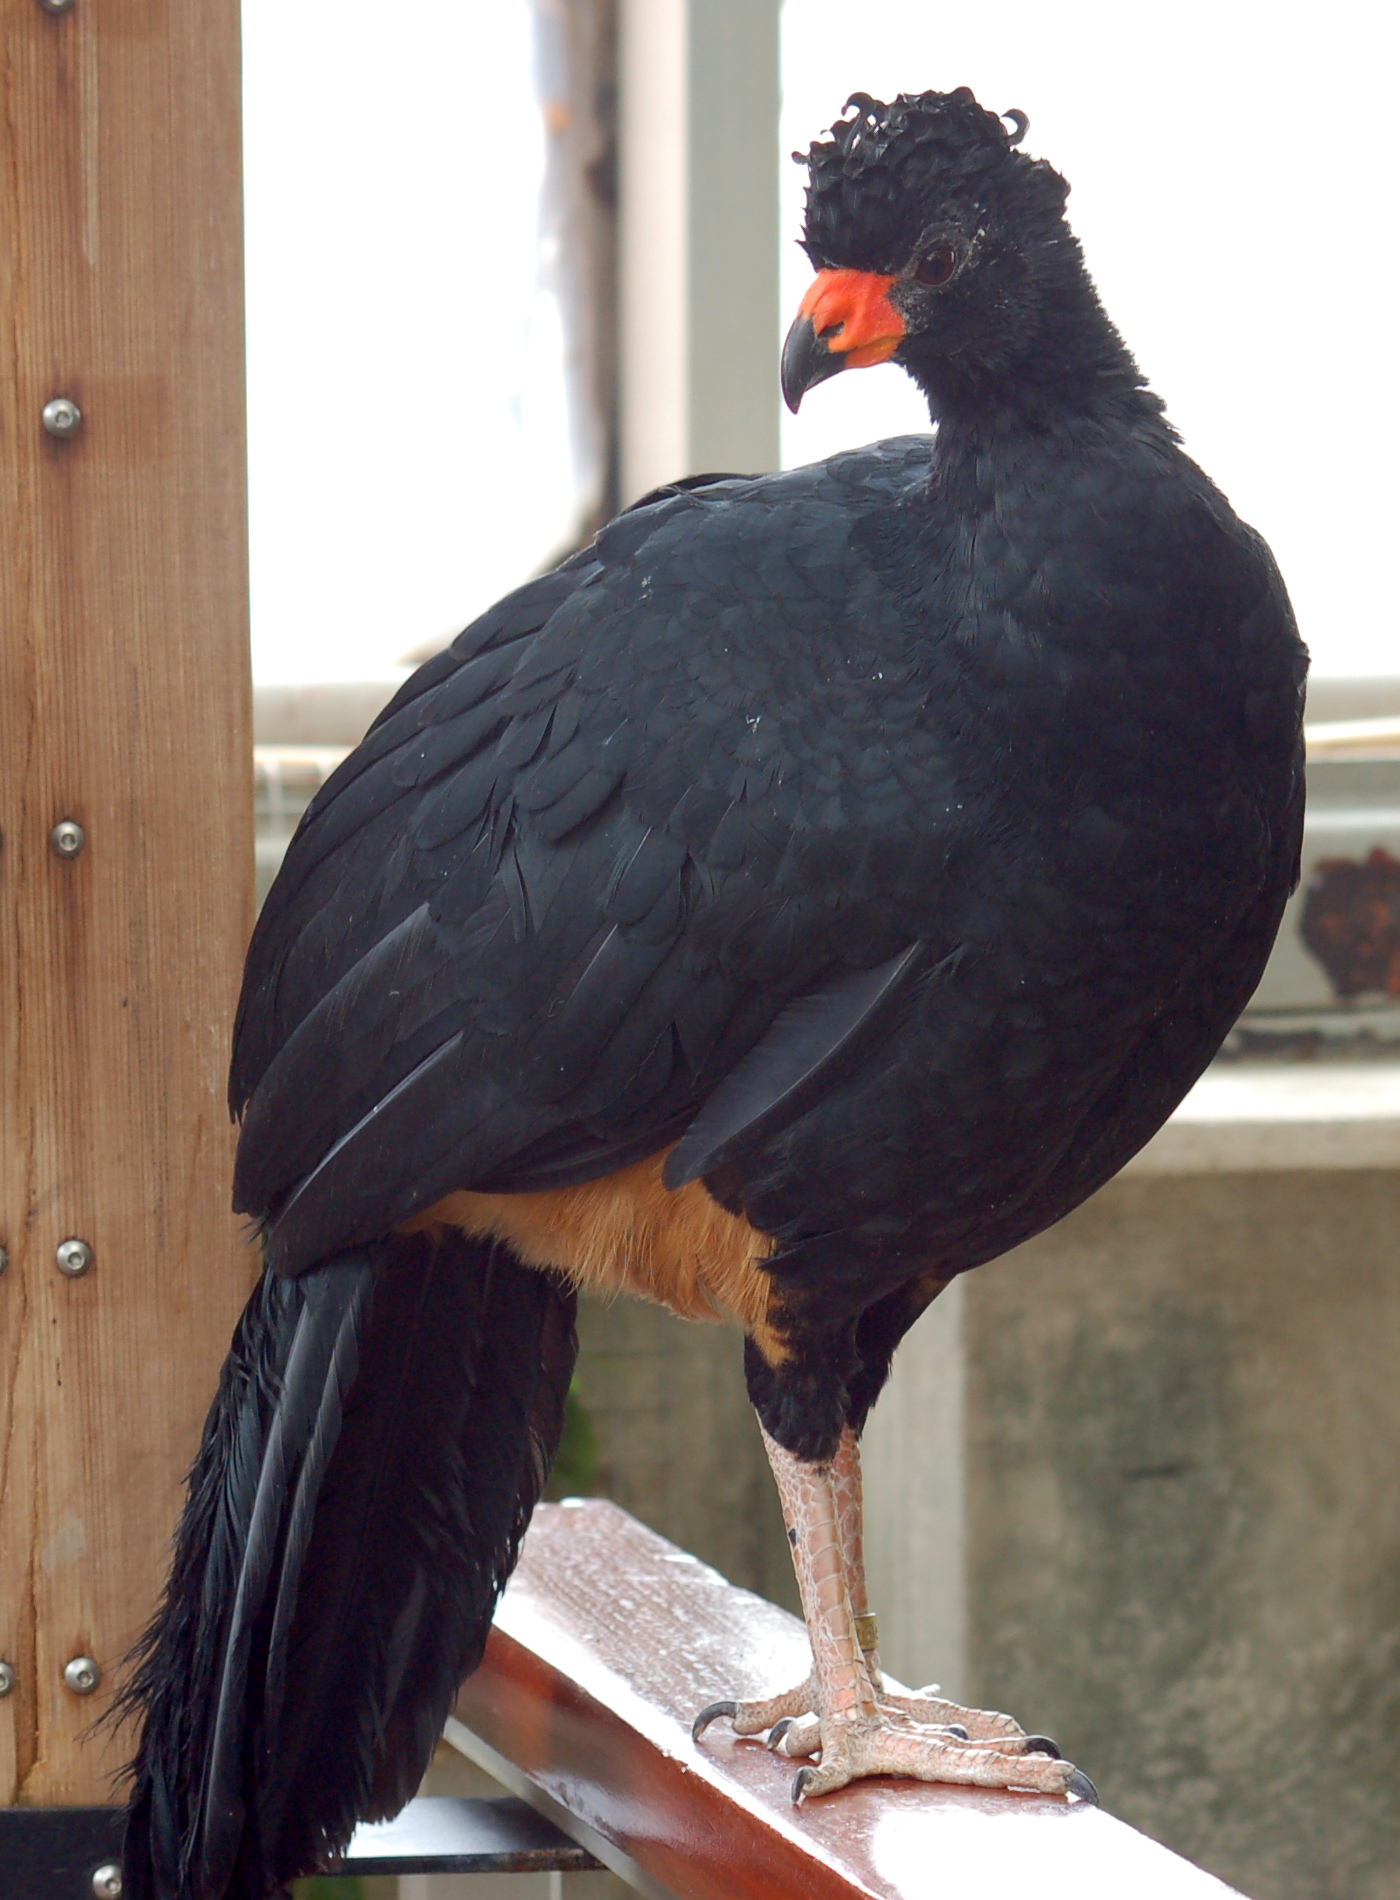
\includegraphics[width=\textwidth,height=4cm,keepaspectratio]{img/foto_crax_globulosa.jpg}
    \caption*{\footnotesize\textit{Crax globulosa}\\(EN) prob=0,237}
  \end{minipage}\hfill
  \begin{minipage}[t]{0.18\textwidth}\centering
    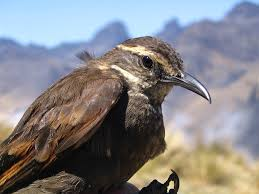
\includegraphics[width=\textwidth,height=4cm,keepaspectratio]{img/foto_cinclodes_aricomae.jpg}
    \caption*{\footnotesize\textit{Cinclodes aricomae}\\(CR) prob=0,230}
  \end{minipage}\hfill
  \begin{minipage}[t]{0.18\textwidth}\centering
    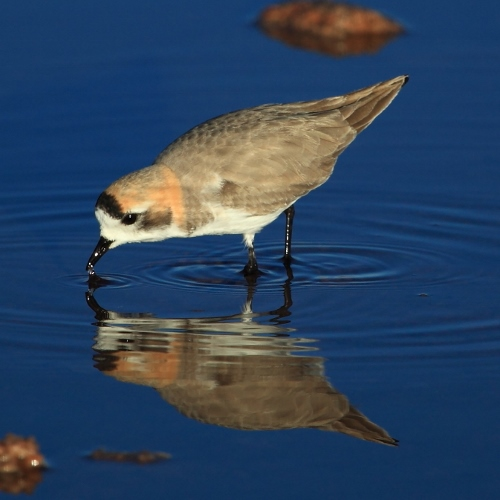
\includegraphics[width=\textwidth,height=4cm,keepaspectratio]{img/foto_charadrius_alticola.jpg}
    \caption*{\footnotesize\textit{Charadrius alticola}\\(---) prob=0,227}
  \end{minipage}\hfill
  \begin{minipage}[t]{0.18\textwidth}\centering
    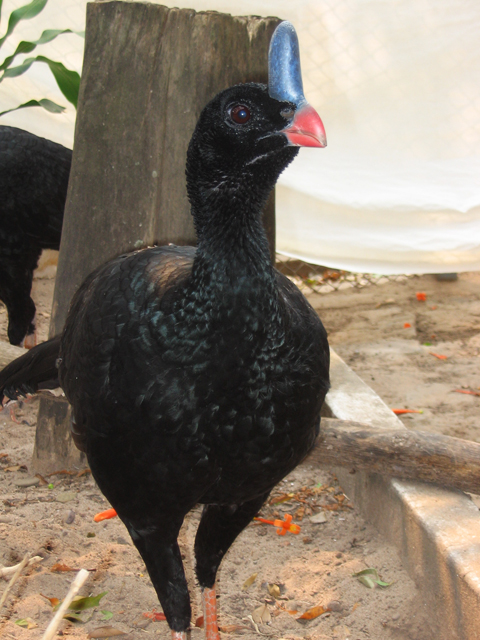
\includegraphics[width=\textwidth,height=4cm,keepaspectratio]{img/foto_pauxi_unicornis.jpg}
    \caption*{\footnotesize\textit{Pauxi unicornis}\\(VU) prob=0,180}
  \end{minipage}\hfill
  \begin{minipage}[t]{0.18\textwidth}\centering
    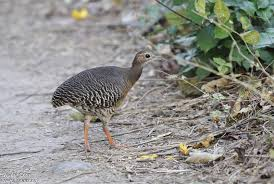
\includegraphics[width=\textwidth,height=4cm,keepaspectratio]{img/foto_taoniscus_nanus.jpg}
    \caption*{\footnotesize\textit{Taoniscus nanus}\\(VU) prob=0,173}
  \end{minipage}
  \caption{Top~5 aves con mayor probabilidad de amenaza predicha por BioAlerta.
           Fuente: Wikimedia Commons / Macaulay Library (CC).}
  \label{fig:fotos_aves_top5}
\end{figure}

\subsubsection{Perfiles detallados --- Top~5 Mamíferos}

\paragraph{\textit{Dasypterus ega} --- Murciélago de cola ancha.}
Quiróptero vespertilionido (familia Vespertilionidae) de distribución neotropical,
con registros dispersos en toda Bolivia.
Aunque su estatus IUCN global es LC (\textit{Least Concern}),
el modelo le asigna la segunda probabilidad más alta en mamíferos (0,283)
después de filtrar especies domésticas.
Este es un \textbf{caso de artefacto por escasez de datos}: los pocos registros bolivianos
en GBIF resultan en pocas ocurrencias por especie, lo que afecta las variables de
densidad de cobertura de la especie.
Su masa corporal relativamente alta para un murciélago insectívoro ($\approx$25--35\,g)
activa el predictor dominante del modelo.
Ilustra la necesidad de complementar las predicciones del modelo con
validación de campo para quirópteros, grupo especialmente sub-muestreado en GBIF.

\paragraph{\textit{Pteronura brasiliensis} --- Londra gigante (VU).}
El mustélido acuático más grande del planeta (hasta 1,8\,m, 32\,kg),
depredador cimero en ríos amazónicos de Bolivia.
Una sola familia puede consumir 3--4\,kg de peces diarios.
Sus poblaciones bolivianas se concentran en los ríos Beni, Iténez, Madre de Dios y
sus afluentes en los departamentos de Beni y Pando.
El \textbf{mercurio de la minería aurífera ilegal} en el Madre de Dios boliviano-peruano
bioacumula en la cadena trófica y llega a concentraciones letales en la londra,
top de la cadena.
La pesca incidental en nasas y redes, la pérdida de playas para reproducción y
la perturbación acústica del tráfico fluvial completan el cuadro de presiones.
El modelo lo detecta correctamente por gran masa, alta dependencia de hábitat
acuático-forestal y distribución en zonas con alta concentración de minería ilegal
(\texttt{pct\_min\_ilegal} y \texttt{min\_ilegal\_dist\_km}).

\paragraph{\textit{Ateles chamek} --- Marimono negro (EN).}
El primate más grande de Bolivia ($\approx$9\,kg), con cola prensil larga que usa como
quinto miembro.
Requiere extensiones de \textbf{bosque maduro continuo} de al menos 100\,km²
para mantener grupos sociales viables; no cruza espacios abiertos, por lo que
carreteras y desmontes actúan como barreras infranqueables para su dispersión.
En Bolivia habita el norte amazónico (Beni, norte de La Paz, Pando).
La caza para consumo de carne de monte ha reducido dramáticamente sus poblaciones en
áreas con acceso vial.
El \textbf{frente de deforestación de la Amazonia boliviana}
---impulsado por la expansión de ganadería y soya hacia el norte del Beni---
amenaza la continuidad del bosque maduro que necesita para sobrevivir.
El modelo activa la predicción por gran masa corporal, alta dependencia de bosque
(\texttt{lc\_forest}), cobertura de concesiones (\texttt{pct\_concesion}) y
distancia corta a vías (\texttt{via\_dist\_km}).

\paragraph{\textit{Inia geoffrensis} --- Bufeo rosado / Delfín rosado (EN).}
Único cetáceo exclusivamente dulceacuícola de la cuenca amazónica boliviana.
Los adultos llegan a superar 2,5\,m y 180\,kg.
En Bolivia habita los ríos Beni, Mamoré, Iténez, Yata, Madre de Dios y Orthon.
La IUCN reclasificó esta especie de \textit{Vulnerable} a \textit{En Peligro} en 2018,
principalmente por el colapso de la población en el Alto Madeira tras las represas.
Las amenazas bolivianas incluyen:
(1) pesca incidental en redes de nylon;
(2) contaminación por mercurio de la minería aurífera en el Madre de Dios;
(3) el proyecto de hidroeléctrica en el Beni (Chepete-El Bala, suspendido pero no descartado);
(4) el dragado del río Beni para tráfico fluvial pesado.
Su masa muy elevada, posición en el tope de la cadena y distribución concentrada en ríos
con alta presión minera explican la predicción del modelo.

\paragraph{\textit{Catagonus wagneri} --- Tagua del Chaco / Pecarí chaqueño (EN).}
Descrita como fósil en 1930 y redescubierta viva en el Gran Chaco paraguayo en 1975,
es la única especie viviente de su género y representa un linaje único no encontrado en
otro lugar de la Tierra.
En Bolivia su distribución se restringe al \textbf{Chaco seco} de Santa Cruz y Chuquisaca.
Con 1--4 crías por camada y una tasa de reclutamiento muy baja, sus poblaciones no
se recuperan rápidamente tras perturbaciones.
La \textbf{expansión ganadera} en el Chaco boliviano ---que implica desmonte masivo de
bosque xerofítico para pastos--- es su amenaza principal.
La caza furtiva y el tráfico de individuos vivos para el mercado de mascotas añaden presión.
El modelo detecta el riesgo por masa corporal media-alta, restricción a hábitat seco-árido
(\texttt{bio14\_mean} bajo, \texttt{bio15\_mean} alto) y alta fracción de hábitat agrícola
en su zona de distribución.

\begin{figure}[H]
  \centering
  \begin{minipage}[t]{0.18\textwidth}\centering
    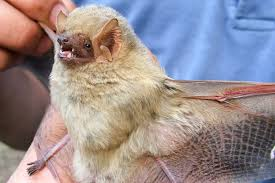
\includegraphics[width=\textwidth,height=4cm,keepaspectratio]{img/foto_dasypterus_ega.jpg}
    \caption*{\footnotesize\textit{Dasypterus ega}\\(LC) prob=0,283}
  \end{minipage}\hfill
  \begin{minipage}[t]{0.18\textwidth}\centering
    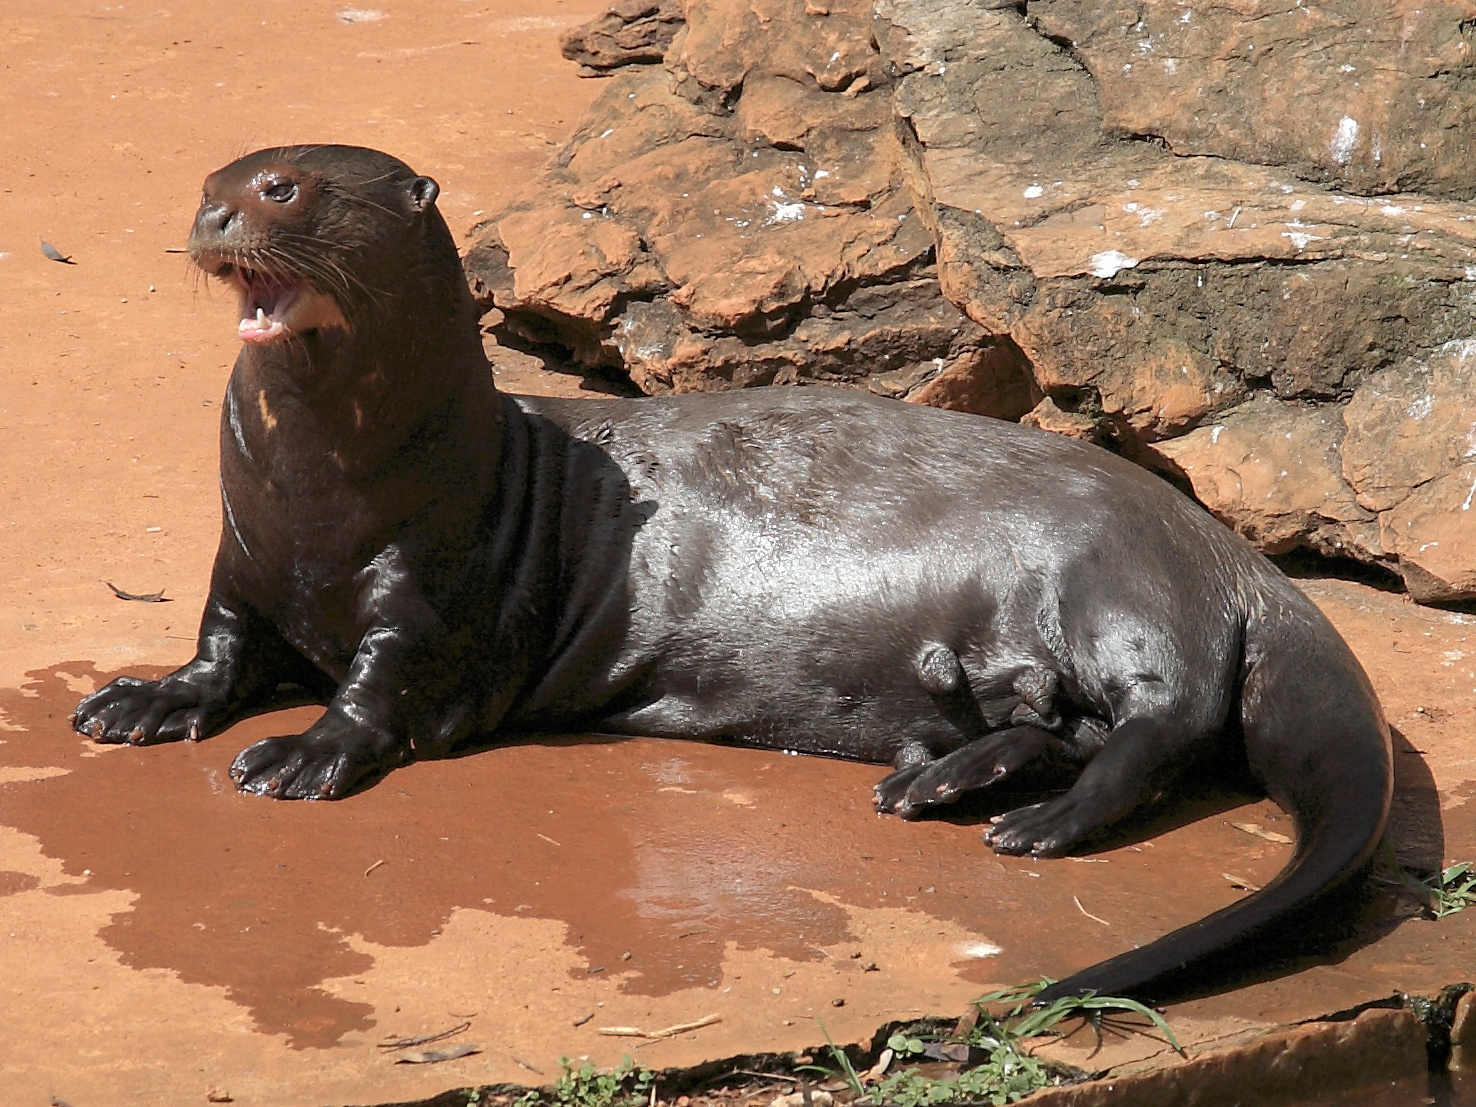
\includegraphics[width=\textwidth,height=4cm,keepaspectratio]{img/foto_pteronura.jpg}
    \caption*{\footnotesize\textit{Pteronura brasiliensis}\\(VU) prob=0,267}
  \end{minipage}\hfill
  \begin{minipage}[t]{0.18\textwidth}\centering
    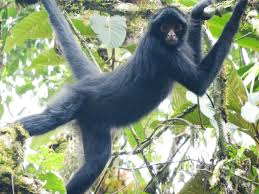
\includegraphics[width=\textwidth,height=4cm,keepaspectratio]{img/foto_ateles_chamek.jpg}
    \caption*{\footnotesize\textit{Ateles chamek}\\(EN) prob=0,220}
  \end{minipage}\hfill
  \begin{minipage}[t]{0.18\textwidth}\centering
    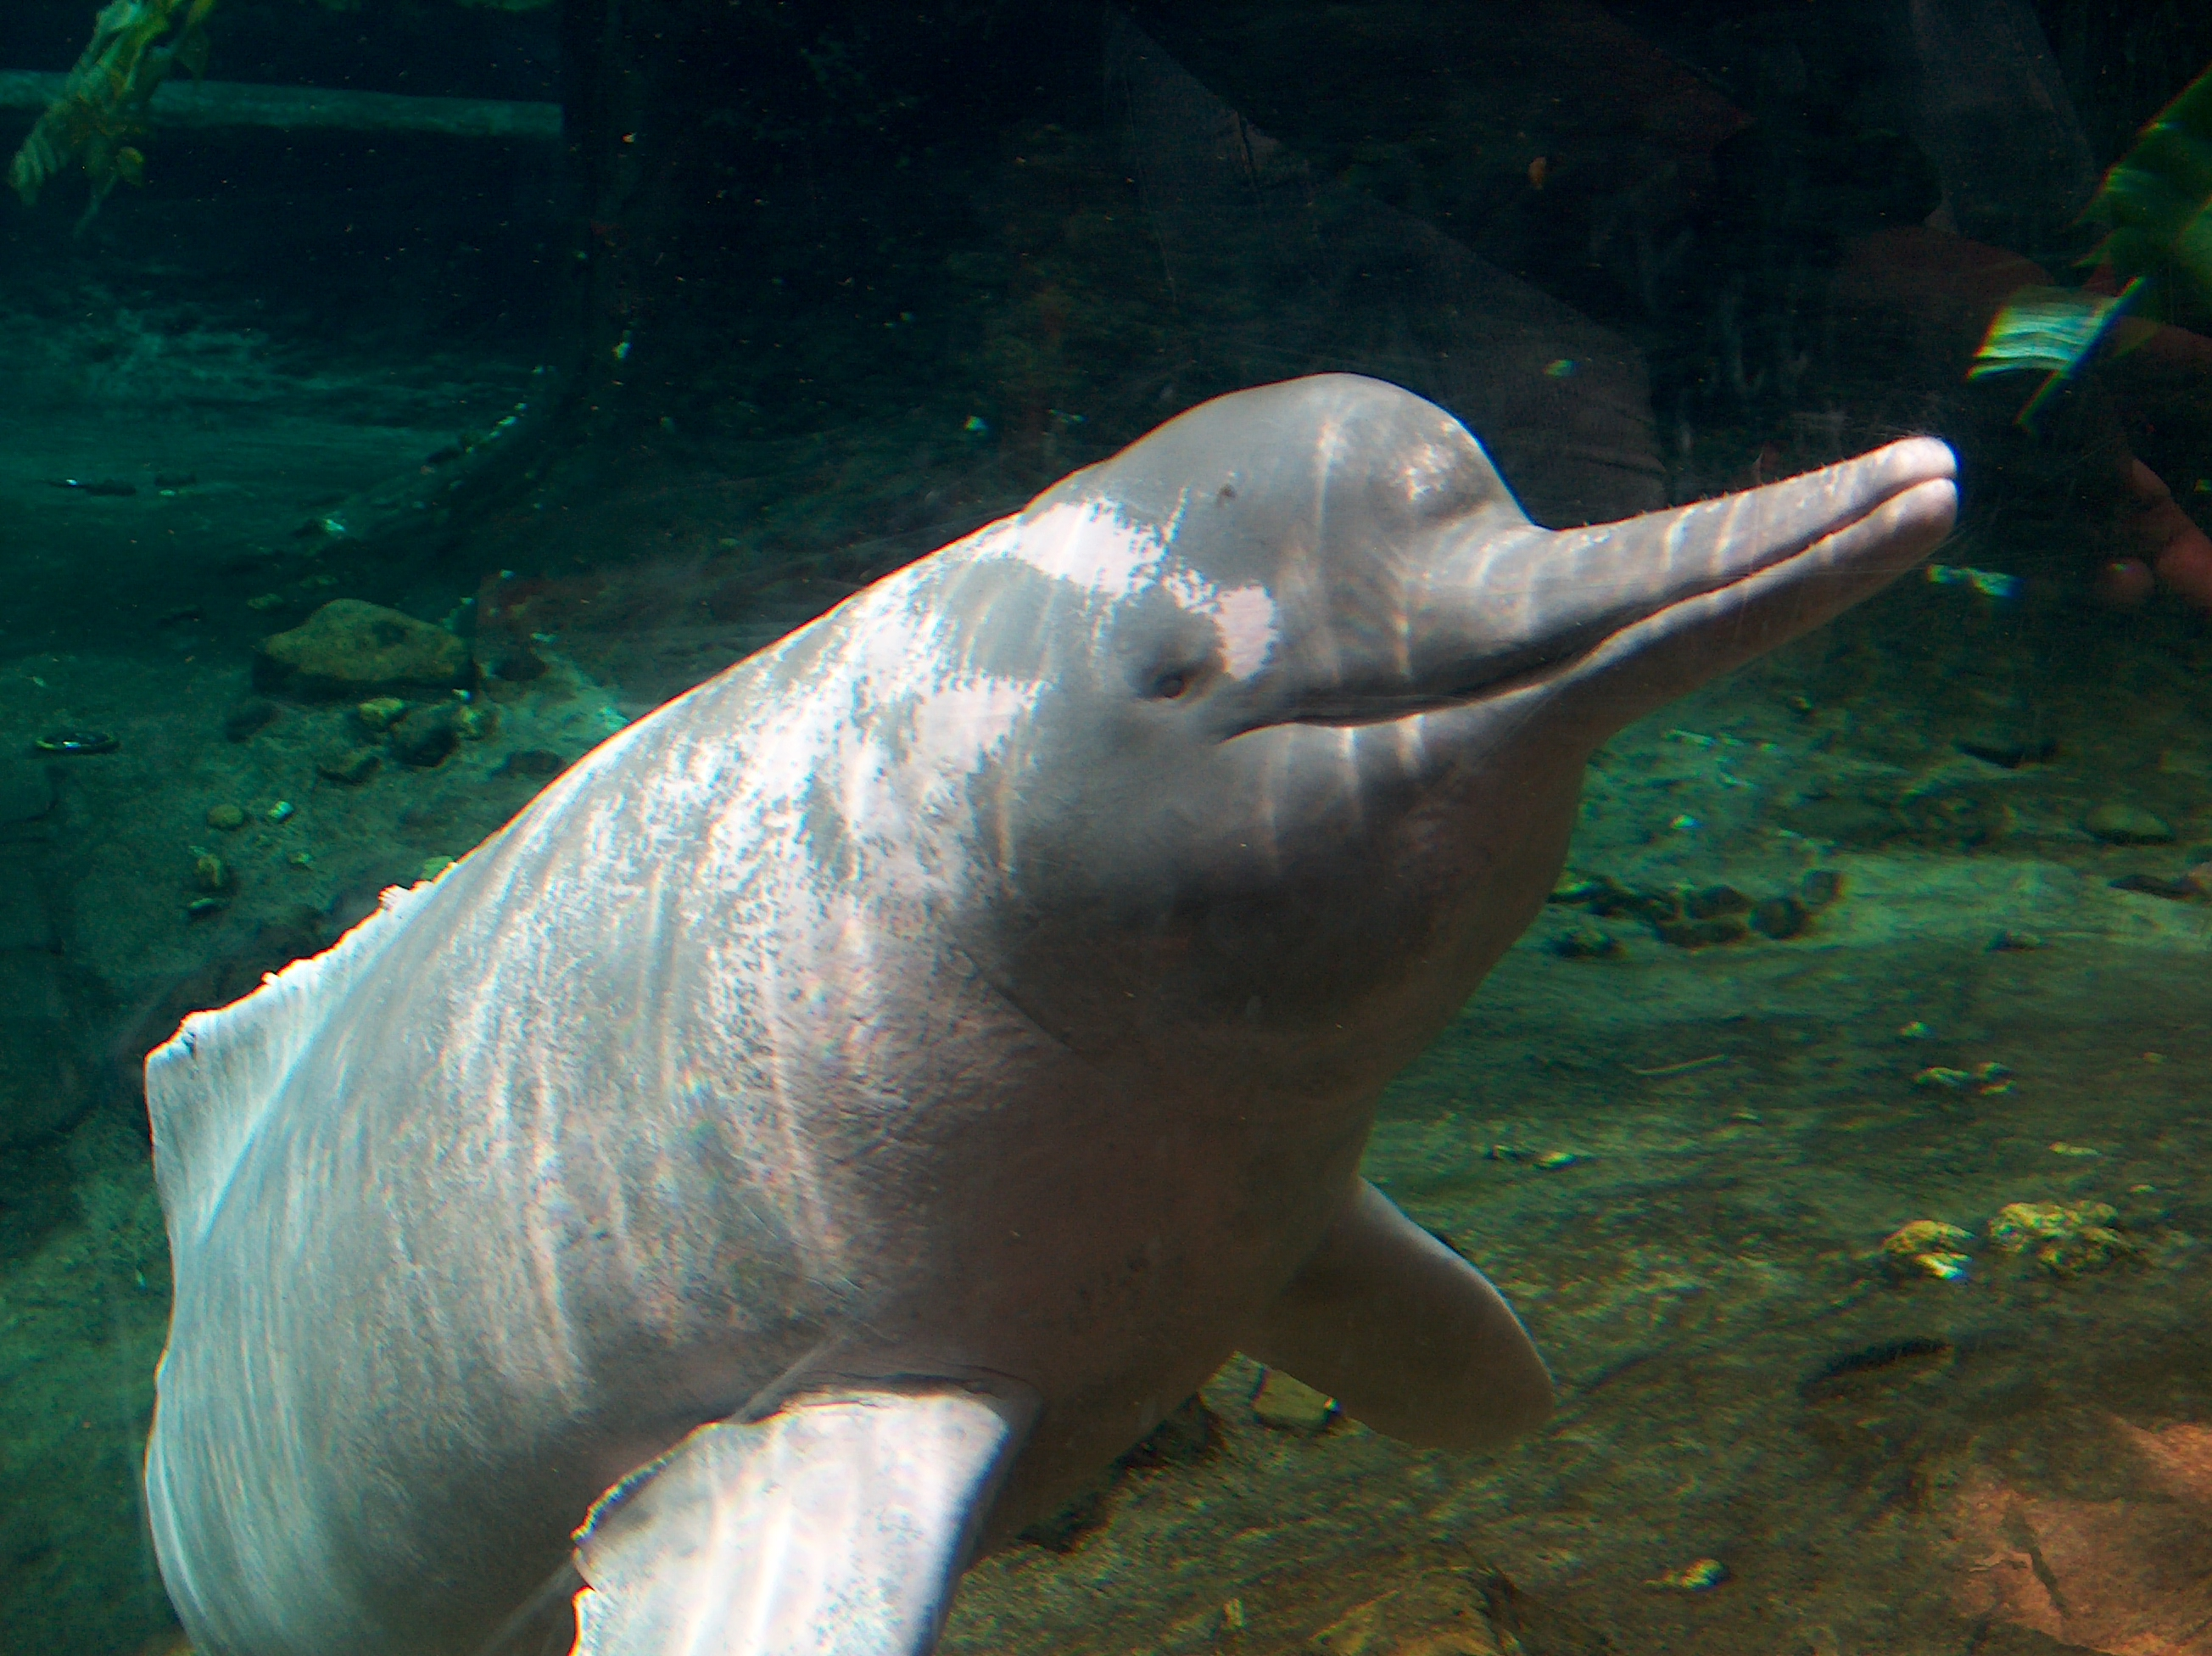
\includegraphics[width=\textwidth,height=4cm,keepaspectratio]{img/foto_inia_geoffrensis.jpg}
    \caption*{\footnotesize\textit{Inia geoffrensis}\\(EN) prob=0,187}
  \end{minipage}\hfill
  \begin{minipage}[t]{0.18\textwidth}\centering
    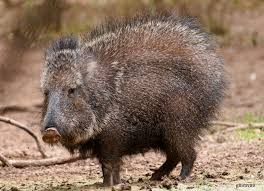
\includegraphics[width=\textwidth,height=4cm,keepaspectratio]{img/foto_catagonus_wagneri.jpg}
    \caption*{\footnotesize\textit{Catagonus wagneri}\\(EN) prob=0,117}
  \end{minipage}
  \caption{Top~5 mamíferos nativos con mayor probabilidad de amenaza predicha por BioAlerta.
           Fuente: Wikimedia Commons / iNaturalist (CC).}
  \label{fig:fotos_mam_top5}
\end{figure}

\subsection{Limitaciones}

\begin{itemize}
  \item \textbf{Especies domésticas en el conjunto de predicción:}
        la ausencia de un filtro por natividad en la construcción del dataset resulta
        en que taxones introducidos (\textit{Ovis aries}, \textit{Bos taurus}) aparezcan
        con probabilidades altas por su masa corporal.
        Un paso de validación con la lista de vertebrados nativos de Bolivia
        (MNHN, 2009) eliminaría estos artefactos.
  \item \textbf{Escasez de datos para mamíferos:} 189 observaciones es un número muy
        reducido para ML; los resultados deben interpretarse como exploratorios.
        Los métodos de aumento de datos (\textit{SMOTE}) o el entrenamiento en un
        corpus latinoamericano más amplio podrían mejorar la capacidad predictiva.
  \item \textbf{Centroide único por especie:} el promediado espacial suaviza la señal
        ambiental local.  Una especie cuyas poblaciones se concentran en una zona
        minera activa pero que también tiene ocurrencias en una ANP remota obtiene
        un centroide lejos del riesgo real.
  \item \textbf{Presión humana no temporal:} las variables de minería, deforestación y
        quemas son estáticas (snapshot 2020--2023) y no capturan la dinámica histórica
        de exposición de cada especie.
  \item \textbf{Sesgo de detección en GBIF:} las especies más registradas tienden a
        ser las más comunes o las más atractivas para observadores ciudadanos (aves
        llamativas, mamíferos grandes), no necesariamente las más amenazadas.
\end{itemize}

\subsection{Trabajo futuro}

\begin{itemize}
  \item \textbf{Filtro de natividad:} excluir del conjunto de predicción las especies
        domésticas/introducidas mediante cruce con listas de fauna nativa boliviana.
  \item \textbf{Calibración de probabilidades:} aplicar \texttt{CalibratedClassifierCV}
        (método isotónico) sobre el Random Forest para obtener probabilidades verdaderamente
        calibradas, complementando el umbral adaptativo ya implementado.
  \item \textbf{Modelado a nivel de poblaciones locales} en lugar de un centroide único
        por especie, lo que permitiría capturar mejor la señal de presión humana y
        detectar especies con distribuciones parcialmente solapadas con focos de riesgo.
  \item \textbf{Modelos de distribución de especies (SDM)} como MaxEnt o BioClim como
        \textit{features} derivadas, reemplazando el centroide puntual por una
        distribución potencial continua para cada especie.
  \item \textbf{Visualización web interactiva} con mapa de Bolivia, puntos de ocurrencia
        coloreados por probabilidad de amenaza predicha, exportados como GeoJSON estáticos.
  \item \textbf{Ampliación temporal:} incorporar series temporales de NDVI (Landsat/MODIS)
        y tasas de deforestación anuales como \textit{features} dinámicas para capturar
        la exposición histórica de cada especie a perturbaciones.
\end{itemize}

%===============================================================
% REFERENCIAS
%===============================================================
\newpage
\begin{thebibliography}{99}

\bibitem{cardillo2004}
Cardillo, M., Mace, G.M., Jones, K.E., et al. (2005).
\textit{Multiple causes of high extinction risk in large mammal species}.
Science, 309(5738), 1239--1241.

\bibitem{bland2015}
Bland, L.M., Collen, B., Orme, C.D.L., \& Bielby, J. (2015).
\textit{Predicting the conservation status of data-deficient species}.
Conservation Biology, 29(1), 250--259.

\bibitem{lee2017}
Lee, T.M., \& Jetz, W. (2011).
\textit{Unravelling the structure of species extinction risk for predictive conservation science}.
Proceedings of the Royal Society B: Biological Sciences, 278(1710), 1329--1338.

\bibitem{szabo2012}
Szabo, J.K., Khwaja, N., Garnett, S.T., \& Butchart, S.H.M. (2012).
\textit{Global patterns and drivers of avian extinctions at the species and subspecies level}.
PLOS ONE, 7(10), e47080.

\bibitem{tobias2022avonet}
Tobias, J.A., Sheard, C., Pigot, A.L., et al. (2022).
\textit{AVONET: morphological, ecological and geographical data for all birds}.
Ecology Letters, 25(3), 581--597.

\bibitem{jones2009pantheria}
Jones, K.E., Bielby, J., Cardillo, M., et al. (2009).
\textit{PanTHERIA: a species-level database of life history, ecology, and geography of extant and recently extinct mammals}.
Ecology, 90(9), 2648.

\bibitem{fick2017worldclim}
Fick, S.E., \& Hijmans, R.J. (2017).
\textit{WorldClim 2: new 1-km spatial resolution climate surfaces for global land areas}.
International Journal of Climatology, 37(12), 4302--4315.

\bibitem{hansen2013gfw}
Hansen, M.C., Potapov, P.V., Moore, R., et al. (2013).
\textit{High-resolution global maps of 21st-century forest cover change}.
Science, 342(6160), 850--853.

\end{thebibliography}

%===============================================================
% ANEXOS
%===============================================================
\newpage
\appendix

\section{Descripción completa de variables del dataset}
\label{anx:features}

\begin{longtable}{p{4.5cm}p{1.8cm}p{6.5cm}}
  \caption{Todas las variables del dataset y su descripción.} \label{tab:all_features} \\
  \toprule
  \textbf{Variable} & \textbf{Tipo} & \textbf{Descripción} \\
  \midrule
  \endfirsthead
  \toprule
  \textbf{Variable} & \textbf{Tipo} & \textbf{Descripción} \\
  \midrule
  \endhead
  \midrule
  \multicolumn{3}{r}{\textit{Continúa en la siguiente página}} \\
  \endfoot
  \bottomrule
  \endlastfoot
  % Climáticas
  bio1\_mean          & Numérica & Temperatura media anual (WorldClim BIO1) \\
  bio4\_mean          & Numérica & Estacionalidad de temperatura (BIO4) \\
  bio7\_mean          & Numérica & Rango de temperatura anual (BIO7) \\
  bio12\_mean         & Numérica & Precipitación anual (BIO12) \\
  bio14\_mean         & Numérica & Precipitación mes más seco (BIO14) \\
  bio15\_mean         & Numérica & Estacionalidad de precipitación (BIO15) \\
  % Deforestación
  pct\_forest\_loss\_total  & Numérica & \% píxeles con pérdida forestal 2001--2023 (GFW) \\
  pct\_forest\_loss\_recent & Numérica & \% píxeles con pérdida forestal 2015--2023 (GFW) \\
  % Cobertura
  lc\_forest          & Numérica & \% ocurrencias en píxeles de bosque (MapBiomas) \\
  lc\_natural         & Numérica & \% ocurrencias en vegetación natural \\
  lc\_agriculture     & Numérica & \% ocurrencias en áreas agrícolas \\
  lc\_water           & Numérica & \% ocurrencias en cuerpos de agua \\
  % Protección
  pct\_anp            & Numérica & \% ocurrencias dentro de ANP \\
  anp\_dist\_km       & Numérica & Distancia al ANP más cercano (km) \\
  pct\_ti             & Numérica & \% ocurrencias dentro de Territorio Indígena \\
  ti\_dist\_km        & Numérica & Distancia al TI más cercano (km) \\
  % Presión minera
  pct\_min\_ilegal    & Numérica & \% ocurrencias en zona de minería ilegal \\
  min\_ilegal\_dist\_km & Numérica & Distancia a minería ilegal más cercana (km) \\
  pct\_concesion      & Numérica & \% ocurrencias en concesiones mineras \\
  concesion\_dist\_km & Numérica & Distancia a concesión minera más cercana (km) \\
  % Petróleo
  pct\_petroleo       & Numérica & \% ocurrencias en bloques petroleros \\
  petroleo\_dist\_km  & Numérica & Distancia al bloque petrolero más cercano (km) \\
  % Accesibilidad
  via\_dist\_km       & Numérica & Distancia a vía nacional más cercana (km) \\
  % Perturbación
  quemas\_freq        & Numérica & Frecuencia media de quemas en zona de ocurrencia \\
  % Meta
  n\_occ              & Numérica & Número de registros de ocurrencia en GBIF \\
  lat\_centroid       & Numérica & Latitud del centroide de distribución \\
  lon\_centroid       & Numérica & Longitud del centroide de distribución \\
  \midrule
  \multicolumn{3}{l}{\textit{Rasgos biológicos --- Aves (AVONET):}} \\
  Mass                & Numérica   & Masa corporal (g) \\
  Beak.Length\_Culmen & Numérica   & Longitud del pico (mm) \\
  Beak.Width          & Numérica   & Ancho del pico (mm) \\
  Beak.Depth          & Numérica   & Profundidad del pico (mm) \\
  Tarsus.Length       & Numérica   & Longitud del tarso (mm) \\
  Wing.Length         & Numérica   & Longitud del ala (mm) \\
  Kipps.Distance      & Numérica   & Índice de forma del ala \\
  Habitat.Density     & Numérica   & Densidad del hábitat preferido \\
  Range.Size          & Numérica   & Tamaño del rango geográfico (km²) \\
  Habitat\_*          & OHE        & Tipo de hábitat (k categorías, k-1 columnas) \\
  Migration\_*        & OHE        & Patrón migratorio \\
  Trophic.Level\_*    & OHE        & Nivel trófico \\
  Trophic.Niche\_*    & OHE        & Nicho trófico detallado \\
  Primary.Lifestyle\_* & OHE       & Estilo de vida principal \\
  \midrule
  \multicolumn{3}{l}{\textit{Rasgos biológicos --- Mamíferos (PanTHERIA):}} \\
  body\_mass\_g       & Numérica & Masa corporal adulta (g) \\
  trophic\_level      & Numérica & Nivel trófico (1=herbívoro, 2=omnívoro, 3=carnívoro) \\
  activity\_cycle     & Numérica & Ciclo de actividad (1=nocturno, 2=cathemeral, 3=diurno) \\
  range\_area\_km2    & Numérica & Área del rango geográfico (km²) \\
  \midrule
  \textbf{threatened} & \textbf{Binaria} & \textbf{TARGET: 1=amenazada, 0=no amenazada} \\
\end{longtable}

\section{Rangos válidos de variables bioclimáticas WorldClim v2.1}
\label{anx:worldclim}

\begin{table}[H]
  \centering\small
  \caption{Rangos físicamente posibles empleados para limpieza de nodata.}
  \begin{tabular}{llcc}
    \toprule
    \textbf{Variable} & \textbf{Descripción} & \textbf{Mín.} & \textbf{Máx.} \\
    \midrule
    bio1\_mean  & Temperatura media anual $\times 10$    & $-600$ & $400$  \\
    bio4\_mean  & Estacionalidad de temperatura $\times 100$ & $0$ & $23000$ \\
    bio7\_mean  & Rango de temperatura anual $\times 10$ & $0$ & $7200$ \\
    bio12\_mean & Precipitación anual (mm)               & $0$ & $12000$ \\
    bio14\_mean & Precipitación mes más seco (mm)        & $0$ & $3000$ \\
    bio15\_mean & Estacionalidad de precipitación (CV)   & $0$ & $265$ \\
    \bottomrule
  \end{tabular}
\end{table}

\section{Resultados completos de validación cruzada}
\label{anx:resultados_full}

Las tablas \ref{tab:resultados_aves} y \ref{tab:resultados_mam} del cuerpo principal
presentan los valores medios de ROC-AUC, PR-AUC y F1-macro.
Las desviaciones estándar entre pliegues reflejan la variabilidad debida al tamaño
reducido del conjunto (especialmente en mamíferos con n=189).

Para interpretar correctamente las métricas con desbalance severo:
\begin{itemize}[nosep]
  \item \textbf{ROC-AUC = 0,848} para aves indica que el modelo asigna probabilidad mayor
        a una especie amenazada que a una no amenazada en el 84,8\,\% de los pares.
  \item \textbf{PR-AUC = 0,192} para aves (vs. la línea base de 0,027 = prevalencia de
        la clase positiva) indica que el modelo tiene 7 veces más precisión que la
        asignación aleatoria para la clase amenazada.
  \item \textbf{F1-macro bajo} ($\approx 0,13$) refleja la dificultad de identificar
        correctamente la clase minoritaria incluso con pesos balanceados.
\end{itemize}

\section{Predicciones completas para especies sin evaluación IUCN}
\label{anx:predicciones}

Las siguientes tablas listan las \textbf{202 especies} (165 aves + 37 mamíferos) sin
evaluación IUCN recuperada vía Wikidata, ordenadas por probabilidad de amenaza predicha
(\texttt{prob\_threatened}) de forma descendente.
La columna \textbf{Pred.} indica la predicción binaria con \textbf{umbral adaptativo}
(prevalencia del \textit{train set}): $0{,}027$ para aves y $0{,}069$ para mamíferos.
Son \textbf{31 aves y 18 mamíferos} los que obtienen \texttt{Pred.=1}
(celdas sombreadas en las tablas).
Los valores proceden del modelo Random Forest entrenado sobre el 100\,\% de los datos
con etiqueta, con \texttt{class\_weight=`balanced'} y \texttt{n\_estimators=300}.

\subsubsection*{Aves (165 especies)}

\begin{longtable}{p{6.2cm}cr}
  \caption{Predicciones completas de amenaza --- Aves.} \label{tab:pred_aves} \\
  \toprule
  \textbf{Especie} & \textbf{Prob.} & \textbf{Pred.} \\
  \midrule
  \endfirsthead
  \toprule
  \textbf{Especie} & \textbf{Prob.} & \textbf{Pred.} \\
  \midrule
  \endhead
  \midrule \multicolumn{3}{r}{\textit{Continúa}} \\
  \endfoot
  \bottomrule
  \endlastfoot
  \rowcolor{grisCelda}\textit{Crax globulosa} & 0.237 & \textbf{1} \\
  \rowcolor{grisCelda}\textit{Cinclodes aricomae} & 0.230 & \textbf{1} \\
  \rowcolor{grisCelda}\textit{Charadrius alticola} & 0.227 & \textbf{1} \\
  \rowcolor{grisCelda}\textit{Pauxi unicornis} & 0.180 & \textbf{1} \\
  \rowcolor{grisCelda}\textit{Taoniscus nanus} & 0.173 & \textbf{1} \\
  \rowcolor{grisCelda}\textit{Amazona xanthops} & 0.140 & \textbf{1} \\
  \rowcolor{grisCelda}\textit{Hylophilus muscicapinus} & 0.130 & \textbf{1} \\
  \rowcolor{grisCelda}\textit{Phibalura boliviana} & 0.120 & \textbf{1} \\
  \rowcolor{grisCelda}\textit{Spizaetus isidori} & 0.100 & \textbf{1} \\
  \rowcolor{grisCelda}\textit{Rollandia microptera} & 0.087 & \textbf{1} \\
  \rowcolor{grisCelda}\textit{Nandayus nenday} & 0.083 & \textbf{1} \\
  \rowcolor{grisCelda}\textit{Idiopsar dorsalis} & 0.080 & \textbf{1} \\
  \rowcolor{grisCelda}\textit{Bucco tamatia} & 0.073 & \textbf{1} \\
  \rowcolor{grisCelda}\textit{Upucerthia ruficaudus} & 0.067 & \textbf{1} \\
  \rowcolor{grisCelda}\textit{Schizoeaca helleri} & 0.060 & \textbf{1} \\
  \rowcolor{grisCelda}\textit{Asthenes sclateri} & 0.060 & \textbf{1} \\
  \rowcolor{grisCelda}\textit{Leucophaeus pipixcan} & 0.060 & \textbf{1} \\
  \rowcolor{grisCelda}\textit{Stilpnia meyerdeschauenseei} & 0.053 & \textbf{1} \\
  \rowcolor{grisCelda}\textit{Harpyhaliaetus coronatus} & 0.053 & \textbf{1} \\
  \rowcolor{grisCelda}\textit{Bucco macrodactylus} & 0.050 & \textbf{1} \\
  \rowcolor{grisCelda}\textit{Porzana flaviventer} & 0.047 & \textbf{1} \\
  \rowcolor{grisCelda}\textit{Xenopipo unicolor} & 0.047 & \textbf{1} \\
  \rowcolor{grisCelda}\textit{Stilpnia cayana} & 0.043 & \textbf{1} \\
  \rowcolor{grisCelda}\textit{Cyanocompsa brissonii} & 0.043 & \textbf{1} \\
  \rowcolor{grisCelda}\textit{Agriornis andicola} & 0.040 & \textbf{1} \\
  \rowcolor{grisCelda}\textit{Ramphocaenus sticturus} & 0.037 & \textbf{1} \\
  \rowcolor{grisCelda}\textit{Cercomacra nigrescens} & 0.037 & \textbf{1} \\
  \rowcolor{grisCelda}\textit{Sporophila maximiliani} & 0.037 & \textbf{1} \\
  \rowcolor{grisCelda}\textit{Oressochen jubatus} & 0.037 & \textbf{1} \\
  \rowcolor{grisCelda}\textit{Phyllomyias uropygialis} & 0.033 & \textbf{1} \\
  \rowcolor{grisCelda}\textit{Chlorestes notata} & 0.030 & \textbf{1} \\
  \textit{Myiophobus ochraceiventris} & 0.027 & 0 \\
  \textit{Myrmeciza hyperythra} & 0.027 & 0 \\
  \textit{Elaenia chilensis} & 0.023 & 0 \\
  \textit{Nystalus striatipectus} & 0.023 & 0 \\
  \textit{Serpophaga munda} & 0.023 & 0 \\
  \textit{Anthus chii} & 0.020 & 0 \\
  \textit{Tachycineta leucopyga} & 0.017 & 0 \\
  \textit{Cyanocompsa rothschildii} & 0.017 & 0 \\
  \textit{Himantopus mexicanus} & 0.013 & 0 \\
  \textit{Hyloctistes subulatus} & 0.013 & 0 \\
  \textit{Loriotus rufiventer} & 0.013 & 0 \\
  \textit{Saltatricula atricollis} & 0.013 & 0 \\
  \textit{Pyrocephalus obscurus} & 0.013 & 0 \\
  \textit{Oceanodroma markhami} & 0.013 & 0 \\
  \textit{Synallaxis propinqua} & 0.013 & 0 \\
  \textit{Chroicocephalus serranus} & 0.010 & 0 \\
  \textit{Leucopternis schistaceus} & 0.010 & 0 \\
  \textit{Leucophaeus atricilla} & 0.010 & 0 \\
  \textit{Gallinula melanops} & 0.010 & 0 \\
  \textit{Loriotus cristatus} & 0.010 & 0 \\
  \textit{Picoides fumigatus} & 0.010 & 0 \\
  \textit{Megascops roraimae} & 0.010 & 0 \\
  \textit{Terenura humeralis} & 0.010 & 0 \\
  \textit{Stilpnia viridicollis} & 0.010 & 0 \\
  \textit{Sturnella militaris} & 0.010 & 0 \\
  \textit{Cranioleuca gutturata} & 0.010 & 0 \\
  \textit{Grallaria sinaensis} & 0.010 & 0 \\
  \textit{Gymnopithys salvini} & 0.007 & 0 \\
  \textit{Geothlypis velata} & 0.007 & 0 \\
  \textit{Chlorothraupis frenata} & 0.007 & 0 \\
  \textit{Phalaropus tricolor} & 0.007 & 0 \\
  \textit{Xenops milleri} & 0.007 & 0 \\
  \textit{Percnostola lophotes} & 0.007 & 0 \\
  \textit{Aratinga aurea} & 0.007 & 0 \\
  \textit{Haplochelidon andecola} & 0.007 & 0 \\
  \textit{Dryocopus schulzii} & 0.007 & 0 \\
  \textit{Harpyhaliaetus solitarius} & 0.007 & 0 \\
  \textit{Himantopus melanurus} & 0.007 & 0 \\
  \textit{Cercomacra serva} & 0.007 & 0 \\
  \textit{Charadrius collaris} & 0.007 & 0 \\
  \textit{Piranga lutea} & 0.007 & 0 \\
  \textit{Myrmeciza goeldii} & 0.007 & 0 \\
  \textit{Schistocichla humaythae} & 0.007 & 0 \\
  \textit{Schistocichla brunneiceps} & 0.007 & 0 \\
  \textit{Myrmeciza atrothorax} & 0.003 & 0 \\
  \textit{Leptasthenura yanacensis} & 0.003 & 0 \\
  \textit{Agelaioides oreopsar} & 0.003 & 0 \\
  \textit{Anthus brevirostris} & 0.003 & 0 \\
  \textit{Anurolimnas viridis} & 0.003 & 0 \\
  \textit{Nystalus obamai} & 0.003 & 0 \\
  \textit{Neochelidon tibialis} & 0.003 & 0 \\
  \textit{Myrmeciza fortis} & 0.003 & 0 \\
  \textit{Philydor ruficaudatum} & 0.003 & 0 \\
  \textit{Strix albitarsis} & 0.003 & 0 \\
  \textit{Thraupis episcopus} & 0.003 & 0 \\
  \textit{Trogon ramonianus} & 0.003 & 0 \\
  \textit{Strix huhula} & 0.003 & 0 \\
  \textit{Xiphorhynchus picus} & 0.003 & 0 \\
  \textit{Upucerthia certhioides} & 0.003 & 0 \\
  \textit{Pteroglossus mariae} & 0.003 & 0 \\
  \textit{Schistocichla leucostigma} & 0.003 & 0 \\
  \textit{Piaya minuta} & 0.003 & 0 \\
  \textit{Pipra rubrocapilla} & 0.003 & 0 \\
  \textit{Sclerurus obscurior} & 0.003 & 0 \\
  \textit{Stilpnia argyrofenges} & 0.003 & 0 \\
  \textit{Atticora melanoleuca} & 0.003 & 0 \\
  \textit{Buteo albicaudatus} & 0.003 & 0 \\
  \textit{Ixothraupis xanthogastra} & 0.003 & 0 \\
  \textit{Idiopsar speculifer} & 0.003 & 0 \\
  \textit{Claravis mondetoura} & 0.003 & 0 \\
  \textit{Leucopternis albicollis} & 0.003 & 0 \\
  \textit{Amazona mercenaria} & 0.000 & 0 \\
  \textit{Anurolimnas castaneiceps} & 0.000 & 0 \\
  \textit{Aramides cajanea} & 0.000 & 0 \\
  \textit{Aratinga acuticaudata} & 0.000 & 0 \\
  \textit{Loriotus luctuosus} & 0.000 & 0 \\
  \textit{Hylophilus hypoxanthus} & 0.000 & 0 \\
  \textit{Idiopsar erythronotus} & 0.000 & 0 \\
  \textit{Ixothraupis punctata} & 0.000 & 0 \\
  \textit{Hylophilus ochraceiceps} & 0.000 & 0 \\
  \textit{Haplospiza rustica} & 0.000 & 0 \\
  \textit{Herpsilochmus frater} & 0.000 & 0 \\
  \textit{Hylocharis sapphirina} & 0.000 & 0 \\
  \textit{Grallaria cochabambae} & 0.000 & 0 \\
  \textit{Elliotomyia chionogaster} & 0.000 & 0 \\
  \textit{Empidonomus aurantioatrocristatus} & 0.000 & 0 \\
  \textit{Chlorestes cyanus} & 0.000 & 0 \\
  \textit{Coccyzus cinereus} & 0.000 & 0 \\
  \textit{Chionomesa lactea} & 0.000 & 0 \\
  \textit{Colibri cyanotus} & 0.000 & 0 \\
  \textit{Dryocopus lineatus} & 0.000 & 0 \\
  \textit{Chionomesa fimbriata} & 0.000 & 0 \\
  \textit{Chalcothraupis ruficervix} & 0.000 & 0 \\
  \textit{Buteo polyosoma} & 0.000 & 0 \\
  \textit{Basileuterus punctipectus} & 0.000 & 0 \\
  \textit{Aratinga mitrata} & 0.000 & 0 \\
  \textit{Aratinga leucophthalma} & 0.000 & 0 \\
  \textit{Percnohierax leucorrhous} & 0.000 & 0 \\
  \textit{Penelope bridgesi} & 0.000 & 0 \\
  \textit{Ochthoeca pulchella} & 0.000 & 0 \\
  \textit{Orthopsittaca manilata} & 0.000 & 0 \\
  \textit{Ocreatus addae} & 0.000 & 0 \\
  \textit{Ochthoeca frontalis} & 0.000 & 0 \\
  \textit{Myrmeciza hemimelaena} & 0.000 & 0 \\
  \textit{Notiochelidon cyanoleuca} & 0.000 & 0 \\
  \textit{Notiochelidon flavipes} & 0.000 & 0 \\
  \textit{Notiochelidon murina} & 0.000 & 0 \\
  \textit{Stilpnia cyanicollis} & 0.000 & 0 \\
  \textit{Rauenia bonariensis} & 0.000 & 0 \\
  \textit{Saltatricula multicolor} & 0.000 & 0 \\
  \textit{Schizoeaca harterti} & 0.000 & 0 \\
  \textit{Pseudoscops clamator} & 0.000 & 0 \\
  \textit{Pseudocolaptes boissonneautii} & 0.000 & 0 \\
  \textit{Psarocolius oseryi} & 0.000 & 0 \\
  \textit{Pionopsitta barrabandi} & 0.000 & 0 \\
  \textit{Porphyrospiza alaudina} & 0.000 & 0 \\
  \textit{Porphyrio martinica} & 0.000 & 0 \\
  \textit{Pitangus lictor} & 0.000 & 0 \\
  \textit{Pipra chloromeros} & 0.000 & 0 \\
  \textit{Pteroglossus beauharnaesii} & 0.000 & 0 \\
  \textit{Phalacrocorax brasilianus} & 0.000 & 0 \\
  \textit{Phylloscartes ophthalmicus} & 0.000 & 0 \\
  \textit{Phylloscartes orbitalis} & 0.000 & 0 \\
  \textit{Xenops rutilans} & 0.000 & 0 \\
  \textit{Troglodytes musculus} & 0.000 & 0 \\
  \textit{Upucerthia harterti} & 0.000 & 0 \\
  \textit{Upucerthia andaecola} & 0.000 & 0 \\
  \textit{Tyto furcata} & 0.000 & 0 \\
  \textit{Thraupis palmarum} & 0.000 & 0 \\
  \textit{Thraupis sayaca} & 0.000 & 0 \\
  \textit{Sturnella superciliaris} & 0.000 & 0 \\
  \textit{Terenura sharpei} & 0.000 & 0 \\
  \textit{Stilpnia nigrocincta} & 0.000 & 0 \\
  \textit{Strix virgata} & 0.000 & 0 \\
\end{longtable}

\bigskip

\subsubsection*{Mamíferos (37 especies)}

\begin{longtable}{p{6.2cm}cr}
  \caption{Predicciones completas de amenaza --- Mamíferos.} \label{tab:pred_mamiferos} \\
  \toprule
  \textbf{Especie} & \textbf{Prob.} & \textbf{Pred.} \\
  \midrule
  \endfirsthead
  \toprule
  \textbf{Especie} & \textbf{Prob.} & \textbf{Pred.} \\
  \midrule
  \endhead
  \midrule \multicolumn{3}{r}{\textit{Continúa}} \\
  \endfoot
  \bottomrule
  \endlastfoot
  \rowcolor{grisCelda}\textit{Ovis aries}$\dagger$ & 0.387 & \textbf{1} \\
  \rowcolor{grisCelda}\textit{Dasypterus ega} & 0.283 & \textbf{1} \\
  \rowcolor{grisCelda}\textit{Equus caballus}$\dagger$ & 0.267 & \textbf{1} \\
  \rowcolor{grisCelda}\textit{Pteronura brasiliensis} & 0.267 & \textbf{1} \\
  \rowcolor{grisCelda}\textit{Bos taurus}$\dagger$ & 0.237 & \textbf{1} \\
  \rowcolor{grisCelda}\textit{Ateles chamek} & 0.220 & \textbf{1} \\
  \rowcolor{grisCelda}\textit{Inia geoffrensis} & 0.187 & \textbf{1} \\
  \rowcolor{grisCelda}\textit{Capra hircus}$\dagger$ & 0.170 & \textbf{1} \\
  \rowcolor{grisCelda}\textit{Bubalus bubalis}$\dagger$ & 0.143 & \textbf{1} \\
  \rowcolor{grisCelda}\textit{Catagonus wagneri} & 0.117 & \textbf{1} \\
  \rowcolor{grisCelda}\textit{Plecturocebus modestus} & 0.113 & \textbf{1} \\
  \rowcolor{grisCelda}\textit{Cyclopes catellus} & 0.110 & \textbf{1} \\
  \rowcolor{grisCelda}\textit{Equus asinus}$\dagger$ & 0.110 & \textbf{1} \\
  \rowcolor{grisCelda}\textit{Sylvilagus brasiliensis} & 0.097 & \textbf{1} \\
  \rowcolor{grisCelda}\textit{Hydrochoeris hydrochaeris} & 0.097 & \textbf{1} \\
  \rowcolor{grisCelda}\textit{Puma yagouaroundi} & 0.073 & \textbf{1} \\
  \rowcolor{grisCelda}\textit{Leopardus braccatus} & 0.073 & \textbf{1} \\
  \rowcolor{grisCelda}\textit{Lama glama}$\dagger$ & 0.070 & \textbf{1} \\
  \textit{Cavia porcellus} & 0.057 & 0 \\
  \textit{Natalus macrourus} & 0.057 & 0 \\
  \textit{Ateles belzebuth} & 0.050 & 0 \\
  \textit{Felis catus} & 0.050 & 0 \\
  \textit{Coendou longicaudatus} & 0.040 & 0 \\
  \textit{Carollia brevicaudum} & 0.027 & 0 \\
  \textit{Abrothrix andinus} & 0.027 & 0 \\
  \textit{Lonchophylla dekeyseri} & 0.023 & 0 \\
  \textit{Marmosops dorothea} & 0.017 & 0 \\
  \textit{Oryctolagus cuniculus} & 0.013 & 0 \\
  \textit{Vicugna pacos} & 0.013 & 0 \\
  \textit{Artibeus glaucus} & 0.007 & 0 \\
  \textit{Cyclopes rufus} & 0.003 & 0 \\
  \textit{Micoureus demerarae} & 0.003 & 0 \\
  \textit{Artibeus gnomus} & 0.000 & 0 \\
  \textit{Hsunycteris thomasi} & 0.000 & 0 \\
  \textit{Eligmodontia hirtipes} & 0.000 & 0 \\
  \textit{Myotis midastactus} & 0.000 & 0 \\
  \textit{Lophostoma silvicola} & 0.000 & 0 \\
\end{longtable}

\end{document}
